%% =====================================================================
%%  MONOGRAFIA DE GRADUACAO EM ENGENHARIA
%%  Desenvolvimento de software orientado por especificacoes (SDD) com
%%  agentes de inteligencia artificial: estudo de caso de um jogo digital
%%  em artefato unico.
%%
%%  IMPORTANTE: este projeto NAO foi validado por compilador. Nao havia
%%  toolchain LaTeX no ambiente de producao (latexmk/pdflatex/xelatex/
%%  tectonic ausentes). Ver MONOGRAFIA_STATUS.md, secao 3.
%%
%%  Compilacao: latexmk -pdf -interaction=nonstopmode -halt-on-error main.tex
%%  Fluxo BibTeX (abntex2cite). NAO usar biber.
%% =====================================================================

\documentclass[
	12pt,				% tamanho da fonte (NBR 14724 pede 12)
	openright,			% capitulos comecam em pagina impar
	oneside,			% monografia: frente e verso iguais
	a4paper,			% papel A4
	brazilian,			% idioma principal
	english,			% idioma secundario (abstract)
	chapter=TITLE,		% capitulos em letras maiusculas (ABNT)
	sumario=abnt-6027-2012,	% formato de sumario conforme NBR 6027
]{abntex2}

%% ---------------------------------------------------------------------
%%  Codificacao, fonte e tipografia
%% ---------------------------------------------------------------------
\usepackage[T1]{fontenc}
\usepackage[utf8]{inputenc}
\usepackage{lmodern}			% fonte vetorial legivel em PDF
\usepackage{textcomp}			% simbolos de texto (graus, etc.)
\usepackage{microtype}			% ajuste fino de composicao
\usepackage{indentfirst}		% indenta o primeiro paragrafo (ABNT)
\usepackage{lastpage}

%% ---------------------------------------------------------------------
%%  Matematica
%% ---------------------------------------------------------------------
\usepackage{amsmath}
\usepackage{amssymb}

%% ---------------------------------------------------------------------
%%  Tabelas e quadros
%% ---------------------------------------------------------------------
\usepackage{booktabs}			% regras horizontais profissionais
\usepackage{longtable}			% tabelas que quebram de pagina
\usepackage{tabularx}			% colunas com largura elastica
\usepackage{array}
\usepackage{multirow}

%% newfloat em vez de float: o pacote float conflita com classes baseadas
%% em memoir (caso da abntex2). newfloat e o substituto recomendado.
\usepackage{newfloat}
\DeclareFloatingEnvironment[
	fileext=loq,
	listname={Lista de quadros},
	name=Quadro,
	placement=htbp,
]{quadro}
%% Nota: o newfloat nomeia a lista a partir do ambiente, gerando
%% \listofquadro. Se a sua distribuicao gerar outro nome (ex.:
%% \listofquadros), ajuste a chamada em chapters/pre-textuais.tex.

%% ---------------------------------------------------------------------
%%  Figuras e diagramas
%% ---------------------------------------------------------------------
\usepackage{graphicx}
%% Alem dos diagramas TikZ em figures/, a monografia inclui a captura de
%% tela real do produto, armazenada em images/ na raiz do repositorio
%% (fonte unica de verdade: o arquivo nao e duplicado dentro da monografia).
\graphicspath{{figures/}{../images/}{images/}}
\usepackage{tikz}
\usetikzlibrary{
	arrows.meta,
	positioning,
	shapes.geometric,
	shapes.misc,
	fit,
	backgrounds,
	calc,
	chains
}

%% ---------------------------------------------------------------------
%%  Listagens de codigo
%% ---------------------------------------------------------------------
%% Snippets inseridos nesta monografia usam apenas caracteres ASCII na
%% area de codigo (seguro com pdflatex + listings). O codigo completo
%% permanece no repositorio, conforme a orientacao da skill.
\usepackage{listings}
\lstdefinestyle{codigo}{
	basicstyle=\ttfamily\footnotesize,
	keywordstyle=\bfseries,
	commentstyle=\itshape,
	breaklines=true,
	breakatwhitespace=false,
	showstringspaces=false,
	tabsize=2,
	columns=fullflexible,
	frame=single,
	framexleftmargin=4pt,
	xleftmargin=6pt,
	numbers=left,
	numberstyle=\tiny,
	numbersep=6pt,
}

%% ---------------------------------------------------------------------
%%  Hipertexto
%% ---------------------------------------------------------------------
%% hyperref e carregado antes do abntex2cite para que as definicoes de
%% citacao do estilo ABNT prevaleçam.
\usepackage{hyperref}
\hypersetup{
	colorlinks=true,
	linkcolor=black,
	citecolor=black,
	urlcolor=black,
	filecolor=black,
	pdftitle={Desenvolvimento de software orientado por especificacoes com agentes de IA},
	pdfauthor={William},
}

%% ---------------------------------------------------------------------
%%  Citacoes no padrao ABNT (autor-data) - NBR 10520
%% ---------------------------------------------------------------------
\usepackage[alf]{abntex2cite}

%% ---------------------------------------------------------------------
%%  Metadados do trabalho
%%
%%  ATENCAO: os campos marcados com [VALIDAR COM O AUTOR] sao dados que
%%  NAO existiam no workspace e NAO foram inventados. Preencha-os antes
%%  da versao final. Ver MONOGRAFIA_PENDENCIAS.md (P-01 a P-07).
%% ---------------------------------------------------------------------
\newcommand{\TrabalhoTitulo}{%
	DESENVOLVIMENTO DE SOFTWARE ORIENTADO POR ESPECIFICAÇÕES COM AGENTES
	DE INTELIGÊNCIA ARTIFICIAL: UM ESTUDO DE CASO APLICADO A UM JOGO
	DIGITAL EM ARTEFATO ÚNICO%
}
\newcommand{\TrabalhoAutor}{William}
\newcommand{\TrabalhoInstituicao}{[VALIDAR COM O AUTOR --- nome da instituição de ensino]}
\newcommand{\TrabalhoUnidade}{[VALIDAR COM O AUTOR --- campus ou unidade]}
\newcommand{\TrabalhoCurso}{[VALIDAR COM O AUTOR --- curso de graduação em Engenharia]}
\newcommand{\TrabalhoOrientador}{[VALIDAR COM O AUTOR --- Prof. Dr. Nome do Orientador]}
\newcommand{\TrabalhoCidade}{[VALIDAR COM O AUTOR --- cidade]}
\newcommand{\TrabalhoAno}{2026}
\newcommand{\TrabalhoNatureza}{%
	Trabalho de Conclusão de Curso apresentado ao curso de
	\TrabalhoCurso\ da \TrabalhoInstituicao\ como requisito parcial para a
	obtenção do título de Engenheiro%
}

%% ---------------------------------------------------------------------
%%  Espacamento e ajustes de composicao
%% ---------------------------------------------------------------------
\setlength{\parindent}{1.3cm}
\setlength{\parskip}{0.2cm}
\renewcommand{\arraystretch}{1.15}

%% Nota de fonte de figuras, tabelas e quadros (padrao ABNT).
%% \providecommand evita conflito caso a classe ja defina \legend.
\providecommand{\legend}[1]{%
	\par\vspace{3pt}%
	{\footnotesize\setlength{\parindent}{0pt}\raggedright #1\par}%
}

%% Evita linhas muito curtas no fim de paragrafos
\widowpenalty=10000
\clubpenalty=10000

%% =====================================================================
\begin{document}

%% ---------------------------------------------------------------------
%%  Elementos pre-textuais
%% ---------------------------------------------------------------------
\pretextual
%% =====================================================================
%%  Elementos pre-textuais
%%  Capa, folha de aprovacao, resumo, abstract, listas e sumario.
%%  Conforme NBR 14724 e NBR 6027.
%%
%%  Os campos entre colchetes sao [VALIDAR COM O AUTOR]: nao existiam no
%%  workspace e nao foram inventados. Ver MONOGRAFIA_PENDENCIAS.md.
%% =====================================================================

%% ---------------------------------------------------------------------
%%  CAPA
%% ---------------------------------------------------------------------
\begin{capa}
	\begin{center}

		\MakeUppercase{\TrabalhoInstituicao}

		\vspace{0.3cm}

		\MakeUppercase{\TrabalhoUnidade}

		\vspace{0.3cm}

		\MakeUppercase{\TrabalhoCurso}

		\vspace{2.5cm}

		\MakeUppercase{\TrabalhoAutor}

		\vspace{3.0cm}

		\textbf{\TrabalhoTitulo}

		\vfill

		\TrabalhoCidade

		\TrabalhoAno

	\end{center}
\end{capa}

%% ---------------------------------------------------------------------
%%  FOLHA DE APROVACAO
%% ---------------------------------------------------------------------
\begin{folhadeaprovacao}
	\begin{center}

		\MakeUppercase{\TrabalhoAutor}

		\vspace{2.0cm}

		\makebox[\textwidth]{\textbf{\TrabalhoTitulo}}

		\vspace{1.5cm}

		\begin{flushright}
			\begin{minipage}{8.5cm}
				\small\SingleSpacing
				\TrabalhoNatureza
				\vspace{0.4cm}

				Orientador: \TrabalhoOrientador
				\vspace{0.4cm}

				Coorientador: [VALIDAR COM O AUTOR --- ou declarar ausência]
			\end{minipage}
		\end{flushright}

		\vspace{1.5cm}

		Aprovado em: \rule{1cm}{0.4pt}/\rule{1cm}{0.4pt}/\rule{1.5cm}{0.4pt}

		\vspace{1.5cm}

		\rule{10cm}{0.4pt}\\
		\TrabalhoOrientador\\
		Presidente da banca --- \TrabalhoInstituicao

		\vspace{1.2cm}

		\rule{10cm}{0.4pt}\\
		\mbox{[VALIDAR COM O AUTOR --- Membro externo/interno 1]}\\
		\mbox{[VALIDAR COM O AUTOR --- titulação e instituição]}

		\vspace{1.2cm}

		\rule{10cm}{0.4pt}\\
		\mbox{[VALIDAR COM O AUTOR --- Membro externo/interno 2]}\\
		\mbox{[VALIDAR COM O AUTOR --- titulação e instituição]}

	\end{center}
\end{folhadeaprovacao}

%% ---------------------------------------------------------------------
%%  DEDICATORIA (opcional - remover se nao for usar)
%% ---------------------------------------------------------------------
%% \begin{dedicatoria}
%% 	\vspace*{\fill}
%% 	\begin{flushright}
%% 		\itshape [VALIDAR COM O AUTOR]
%% 	\end{flushright}
%% 	\vspace*{\fill}
%% \end{dedicatoria}

%% ---------------------------------------------------------------------
%%  AGRADECIMENTOS (opcional - remover se nao for usar)
%% ---------------------------------------------------------------------
%% \begin{agradecimentos}
%% 	[VALIDAR COM O AUTOR]
%% \end{agradecimentos}

%% ---------------------------------------------------------------------
%%  EPIGRAFE (opcional - remover se nao for usar)
%% ---------------------------------------------------------------------
%% \begin{epigrafe}
%% 	\vspace*{\fill}
%% 	\begin{flushright}
%% 		\itshape ``[VALIDAR COM O AUTOR --- citação com autoria]''
%% 	\end{flushright}
%% 	\vspace*{\fill}
%% \end{epigrafe}

%% ---------------------------------------------------------------------
%%  RESUMO - NBR 6028
%% ---------------------------------------------------------------------
\begin{resumo}
	Agentes de inteligência artificial generativa produzem código com alta
	velocidade, mas a ausência de um processo que force especificação prévia,
	critérios de aceitação verificáveis e registro de evidências compromete a
	auditabilidade e a manutenção do que foi produzido. Este trabalho define,
	aplica e avalia um processo de desenvolvimento orientado por especificações
	(\textit{spec-driven development} --- SDD) executado por agentes de
	inteligência artificial, organizado em quinze agentes especializados,
	quatro conjuntos de instruções permanentes e cinco habilidades de domínio,
	com fluxo adaptativo ao risco e seis portões de verificação. O processo foi
	aplicado à construção de um jogo digital completo entregue como artefato
	único de página web, especificado com quinze requisitos funcionais, nove
	requisitos não funcionais e doze critérios de aceitação. A verificação foi
	empírica, combinando inspeção estática do artefato com automação de
	navegador para teclado, apontador e leitura de pixels da área de desenho.
	Os doze critérios de aceitação foram satisfeitos, incluindo o bloqueio de
	inversão de trajetória, o sorteio de alvos fora do corpo do jogador e a
	persistência do recorde no armazenamento local. Mediu-se ainda o intervalo
	entre passos de simulação em duas faixas de pontuação: 133\,ms para
	pontuação inferior a quarenta pontos e 105\,ms para pontuação igual ou
	superior a oitenta pontos, sobre 184 movimentos amostrados, confirmando o
	aumento de velocidade previsto na especificação. O trabalho identifica como
	limitações a ausência de grupo de controle, a extensão reduzida da amostra
	temporal, a carência de critérios de aceitação para nove requisitos não
	funcionais e a não validação dos controles de toque em dispositivo físico.
	Conclui-se que o processo proposto torna cada entrega rastreável a um
	requisito e sustentada por evidência reproduzível, ao custo de maior
	disciplina documental.

	\vspace{\onelineskip}

	\noindent
	\textbf{Palavras-chave}: desenvolvimento orientado por especificações;
	agentes de inteligência artificial; engenharia de requisitos; verificação e
	validação; rastreabilidade; estudo de caso.
\end{resumo}

%% ---------------------------------------------------------------------
%%  ABSTRACT - NBR 6028
%% ---------------------------------------------------------------------
\begin{abstract}
	Generative artificial intelligence agents produce code at high speed, yet
	without a process that enforces prior specification, verifiable acceptance
	criteria and recorded evidence, the outcome is hard to audit and to
	maintain. This work defines, applies and evaluates a spec-driven
	development (SDD) process executed by artificial intelligence agents,
	organised into fifteen specialised agents, four permanent instruction sets
	and five domain skills, with a risk-adaptive flow and six verification
	gates. The process was applied to building a complete digital game
	delivered as a single web page artefact, specified with fifteen functional
	requirements, nine non-functional requirements and twelve acceptance
	criteria. Verification was empirical, combining static inspection of the
	artefact with browser automation for keyboard, pointer and pixel reading of
	the drawing surface. All twelve acceptance criteria passed, including
	trajectory reversal blocking, target spawning outside the player's body and
	high-score persistence in local storage. The interval between simulation
	steps was measured across two score bands: 133\,ms below forty points and
	105\,ms at or above eighty points, over 184 sampled movements, confirming
	the speed increase defined in the specification. The work identifies as
	limitations the absence of a control group, the small temporal sample, the
	lack of acceptance criteria for nine non-functional requirements and the
	unvalidated touch controls on physical devices. It concludes that the
	proposed process makes every deliverable traceable to a requirement and
	supported by reproducible evidence, at the cost of greater documentation
	discipline.

	\vspace{\onelineskip}

	\noindent
	\textbf{Keywords}: spec-driven development; artificial intelligence agents;
	requirements engineering; verification and validation; traceability; case
	study.
\end{abstract}

%% ---------------------------------------------------------------------
%%  LISTA DE ILUSTRACOES (figuras)
%% ---------------------------------------------------------------------
\pdfbookmark[0]{\listfigurename}{lof}
\listoffigures
\newpage

%% ---------------------------------------------------------------------
%%  LISTA DE QUADROS
%% ---------------------------------------------------------------------
\pdfbookmark[0]{Lista de quadros}{loq}
\listofquadro
\newpage

%% ---------------------------------------------------------------------
%%  LISTA DE TABELAS
%% ---------------------------------------------------------------------
\pdfbookmark[0]{\listtablename}{lot}
\listoftables
\newpage

%% ---------------------------------------------------------------------
%%  LISTA DE ABREVIATURAS E SIGLAS
%% ---------------------------------------------------------------------
\begin{siglas}
	\item[ABNT] Associação Brasileira de Normas Técnicas
	\item[ADR] \textit{Architecture Decision Record} (registro de decisão arquitetural)
	\item[API] \textit{Application Programming Interface}
	\item[AP] \textit{Access Point} (ponto de acesso sem fio)
	\item[CA] Critério de Aceitação
	\item[CSS] \textit{Cascading Style Sheets}
	\item[DPR] \textit{Device Pixel Ratio} (razão de pixels do dispositivo)
	\item[ECMA] \textit{European Computer Manufacturers Association}
	\item[FR] Requisito Funcional
	\item[FSM] \textit{Finite State Machine} (máquina de estados finitos)
	\item[HTML] \textit{HyperText Markup Language}
	\item[IA] Inteligência Artificial
	\item[ISO] \textit{International Organization for Standardization}
	\item[JSON] \textit{JavaScript Object Notation}
	\item[LLM] \textit{Large Language Model} (modelo de linguagem de grande porte)
	\item[NBR] Norma Brasileira
	\item[NFR] Requisito Não Funcional
	\item[RAM] \textit{Random Access Memory}
	\item[SDD] \textit{Spec-Driven Development}
	\item[SQuaRE] \textit{Software product Quality Requirements and Evaluation}
	\item[SRP] \textit{Single Responsibility Principle}
	\item[TCC] Trabalho de Conclusão de Curso
	\item[UI] \textit{User Interface} (interface do usuário)
	\item[V\&V] Verificação e Validação
	\item[W3C] \textit{World Wide Web Consortium}
	\item[WCAG] \textit{Web Content Accessibility Guidelines}
	\item[WHATWG] \textit{Web Hypertext Application Technology Working Group}
\end{siglas}

%% ---------------------------------------------------------------------
%%  LISTA DE SIMBOLOS
%% ---------------------------------------------------------------------
\begin{simbolos}
	\item[$A$] Conjunto de critérios de aceitação verificados
	\item[$C$] Custo agregado de verificação
	\item[$e$] Número de itens consumidos na partida
	\item[$\mathrm{E}{[}T{]}$] Intervalo médio entre passos de simulação
	\item[$m$] Número de amostras de movimento
	\item[$s$] Pontuação acumulada na partida
	\item[$t_{\max}$] Intervalo máximo entre passos de simulação
	\item[$t_{\min}$] Intervalo mínimo entre passos de simulação
	\item[$t_0$] Intervalo inicial entre passos de simulação
	\item[$\Delta$] Passo de redução do intervalo por item consumido
	\item[$\sigma$] Desvio padrão amostral
\end{simbolos}

%% ---------------------------------------------------------------------
%%  SUMARIO - NBR 6027
%% ---------------------------------------------------------------------
\pdfbookmark[0]{\contentsname}{toc}
\tableofcontents*
\newpage


%% ---------------------------------------------------------------------
%%  Elementos textuais
%% ---------------------------------------------------------------------
\textual

%% =====================================================================
%%  CAPITULO 1 - INTRODUCAO
%% =====================================================================

\chapter{Introdução}
\label{cap:introducao}

Este capítulo apresenta o contexto do trabalho, o problema de engenharia
investigado, a justificativa, a hipótese, os objetivos, a delimitação do escopo,
uma visão resumida do método e a organização dos demais capítulos.

\section{Contextualização}
\label{sec:contextualizacao}

A produção de software assistida por modelos de linguagem de grande porte
(\textit{Large Language Models} --- LLM) deixou de ser experimento de laboratório
e passou a integrar rotinas reais de desenvolvimento. Modelos treinados em larga
escala demonstram capacidade de generalização para tarefas não vistas durante o
treinamento, fenômeno descrito como aprendizado em poucos exemplos
(\citeonline{brown2020}). A arquitetura de atenção
proposta por \citeonline{vaswani2017} viabilizou essa classe de modelos, e
técnicas de encadeamento de raciocínio ampliaram a capacidade de resolução de
problemas estruturados (\citeonline{wei2022}).

A partir dessa base, surgiram abordagens que organizam o modelo como agente
capaz de raciocinar e agir sobre um ambiente (\citeonline{yao2023react}), de
refletir sobre os próprios erros (\citeonline{shinn2023reflexion}) e de operar em
conjunto com outros agentes, cada um com papel especializado
(\citeonline{hong2024metagpt}; \citeonline{qian2024chatdev};
\citeonline{wu2023autogen}).

O ganho de velocidade é evidente; o ganho de qualidade é condicional. Um agente
que recebe um pedido vago produz código plausível, mas plausibilidade não é
corretude. Quando não existe especificação prévia, não há como decidir se o que
foi entregue é o que foi pedido; quando não existem critérios de aceitação, não
há como demonstrar que o pedido foi atendido; e quando não há registro de
evidência, a conclusão depende de confiança, não de verificação. A engenharia de
software já conhecia esse problema: a distinção entre verificação e validação e a
necessidade de critérios objetivos foram formalizadas há décadas
(\citeonline{boehm1984}), e a especificação de requisitos permanece sendo a
atividade com maior impacto sobre o custo final do produto
(\citeonline{sommerville2019}; \citeonline{pressman2016}).

\section{Problema de engenharia}
\label{sec:problema}

O problema investigado é:

\begin{citacao}
	Como estruturar um processo de desenvolvimento assistido por agentes de
	inteligência artificial de modo que cada entrega seja (i) rastreável a um
	requisito, (ii) verificável por um critério de aceitação e (iii) sustentada
	por evidência reproduzível?
\end{citacao}

O problema se decompõe em três dificuldades práticas. A primeira é de natureza
processual: agentes tendem a responder ao pedido mais recente, e não ao contrato
acumulado, de modo que sem um artefato de estado persistente o escopo se degrada
ao longo da execução. A segunda é de natureza epistemológica: a saída de um
agente é texto plausível, e plausibilidade não é evidência; é necessário
distinguir o que foi afirmado do que foi demonstrado. A terceira é de natureza
econômica: quanto maior o volume de contexto carregado, maior o custo e maior a
probabilidade de o agente tratar informação obsoleta como atual.

\section{Justificativa}
\label{sec:justificativa}

A relevância do estudo se sustenta em três argumentos.

\textbf{Argumento de risco.} As práticas que reduzem risco de regressão em
software --- integração contínua, testes automatizados, releases frequentes e
pequenas --- estão associadas a melhor desempenho organizacional
(\citeonline{humble2010}; \citeonline{forsgren2018}). Um processo que aceita
código gerado por agente sem passar pelos mesmos portões de qualidade importa
risco para dentro do produto.

\textbf{Argumento de auditabilidade.} Em domínios regulados ou críticos, a
pergunta relevante não é apenas se o software funciona, mas quem decidiu o quê,
com base em qual requisito e com qual evidência. A rastreabilidade é um requisito
de engenharia, não um subproduto (\citeonline{iso29148}).

\textbf{Argumento de reprodutibilidade.} Se duas execuções do mesmo pedido
produzem resultados diferentes e não existe especificação, o resultado não é
comparável nem acumulável. Sem artefatos congelados, o conhecimento produzido em
uma sessão se perde na seguinte.

Além disso, a literatura sobre agentes LLM aplicados à engenharia de software
concentra-se majoritariamente na geração de código
(\citeonline{hong2024metagpt}; \citeonline{qian2024chatdev}). O presente trabalho
desloca o foco da geração para o \textit{controle}: quais artefatos, portões e
condições de parada tornam a geração auditável.

\section{Hipótese}
\label{sec:hipotese}

A hipótese de trabalho é:

\begin{citacao}
	Um processo que obriga a especificação prévia com requisitos identificados,
	critérios de aceitação testáveis e evidência registrada produz entregas
	verificáveis por terceiros sem acesso ao histórico da conversa, ao custo de
	maior esforço documental.
\end{citacao}

A hipótese é falseável de duas maneiras. Primeiro, se algum critério de aceitação
não puder ser verificado sem consultar o autor, a rastreabilidade proposta
falhou. Segundo, se a evidência registrada não puder ser reproduzida a partir dos
artefatos versionados, o processo não é reprodutível. Ambos os testes foram
aplicados neste trabalho, e os resultados estão no Capítulo~\ref{cap:resultados}.

\section{Objetivos}
\label{sec:objetivos}

\subsection{Objetivo geral}
\label{subsec:objetivo-geral}

Definir, aplicar e avaliar um processo de desenvolvimento orientado por
especificações (\textit{spec-driven development} --- SDD) executado por agentes
de inteligência artificial, utilizando como estudo de caso a construção de um
jogo digital completo entregue em artefato único.

\subsection{Objetivos específicos}
\label{subsec:objetivos-especificos}

\begin{quadro}[htb]
	\caption{Objetivos específicos e critério de sucesso}
	\label{qua:objetivos}
	\centering
	\footnotesize
	\begin{tabularx}{\textwidth}{@{}p{1.1cm} X p{3.4cm}@{}}
		\toprule
		\textbf{ID} & \textbf{Objetivo específico} & \textbf{Critério de sucesso} \\
		\midrule
		OE-1 & Projetar o framework de agentes, instruções e artefatos de controle. & Framework descrito e versionado no repositório. \\
		\addlinespace
		OE-2 & Especificar formalmente o sistema-alvo com requisitos e critérios de aceitação verificáveis. & Todo requisito com identificador único. \\
		\addlinespace
		OE-3 & Registrar as decisões arquiteturais do alvo com alternativas descartadas. & Cada decisão com justificativa e alternativa rejeitada. \\
		\addlinespace
		OE-4 & Implementar o alvo sob as restrições especificadas. & Artefato único, sem dependências externas. \\
		\addlinespace
		OE-5 & Verificar cada critério de aceitação com evidência empírica. & Um resultado observável por critério. \\
		\addlinespace
		OE-6 & Avaliar o processo, suas limitações e ameaças à validade. & Ameaças classificadas e dados ausentes marcados. \\
		\bottomrule
	\end{tabularx}
	\legend{Fonte: elaborado pelo autor (2026).}
\end{quadro}

\section{Delimitação do escopo}
\label{sec:delimitacao}

\textbf{Dentro do escopo:} o processo de desenvolvimento, sua especificação,
sua aplicação a um sistema-alvo e a verificação empírica do alvo.

\textbf{Fora do escopo:} o treinamento ou a avaliação comparativa de modelos de
linguagem; a medição de custo financeiro por execução; a avaliação de usabilidade
com usuários humanos; e a comparação experimental contra grupo de controle, que
exigiria um segundo desenvolvimento paralelo do mesmo alvo.

Registra-se ainda uma delimitação factual relevante. O repositório onde o
trabalho foi conduzido contém a descrição de um sistema embarcado de controle
térmico, sem código, medição ou resultado correspondente. Como não há evidência
empírica desse sistema, ele não é objeto deste estudo; o estudo de caso é o
produto efetivamente implementado e verificado. Essa inconsistência documental
está registrada em \texttt{MONOGRAFIA\_PENDENCIAS.md} (P-26).

\section{Visão resumida do método}
\label{sec:metodo-resumido}

O trabalho é um estudo de caso único, de natureza aplicada, com abordagem
qualitativa predominante e componentes quantitativos pontuais
(\citeonline{yin2018}; \citeonline{runeson2009}). O procedimento teve quatro
etapas: (i) projeto do framework de agentes a partir das lacunas identificadas
em uma avaliação crítica prévia do material de origem; (ii) especificação do
alvo com requisitos funcionais, não funcionais e critérios de aceitação;
(iii) implementação sob restrições declaradas; e (iv) verificação empírica em
navegador, com inspeção estática e automação. O detalhamento está no
Capítulo~\ref{cap:metodos}.

\section{Organização do trabalho}
\label{sec:organizacao}

O Capítulo~\ref{cap:fundamentacao} apresenta a fundamentação teórica em
engenharia de software e agentes de inteligência artificial. O
Capítulo~\ref{cap:relacionados} compara trabalhos correlatos. O
Capítulo~\ref{cap:metodos} descreve materiais e métodos, incluindo ameaças à
validade. O Capítulo~\ref{cap:framework} detalha o framework SDD agêntico
proposto. O Capítulo~\ref{cap:especificacao} apresenta a especificação do
sistema-alvo. O Capítulo~\ref{cap:implementacao} descreve a implementação e suas
decisões arquiteturais. O Capítulo~\ref{cap:resultados} reporta experimentos e
resultados. O Capítulo~\ref{cap:discussao} discute os achados e as limitações. O
Capítulo~\ref{cap:conclusao} conclui e indica trabalhos futuros.

%% =====================================================================
%%  CAPITULO 2 - FUNDAMENTACAO TEORICA
%% =====================================================================

\chapter{Fundamentação Teórica}
\label{cap:fundamentacao}

Este capítulo estabelece os conceitos necessários para compreender o problema e a
solução proposta. A primeira parte trata de engenharia de software --- ciclo de
vida, requisitos, verificação e validação, testes e qualidade. A segunda trata de
agentes de inteligência artificial --- modelos de linguagem, agentes autônomos e
sistemas multiagente. A terceira trata do domínio de aplicação. A seção final
sintetiza as duas áreas e identifica a lacuna que o trabalho aborda.

\section{Engenharia de software e ciclo de vida}
\label{sec:ciclo-de-vida}

Engenharia de software é a aplicação de abordagem sistemática, disciplinada e
quantificável ao desenvolvimento, operação e manutenção de software
(\citeonline{sommerville2019}). A palavra decisiva é \emph{sistemática}: a
diferença entre programar e engenhar software está na existência de um processo
que torne o resultado previsível e inspecionável.

Processos de desenvolvimento organizam-se tradicionalmente em fases ---
elicitação, análise, projeto, implementação, teste, implantação e manutenção ---
ainda que a execução real raramente seja estritamente sequencial
(\citeonline{pressman2016}). Modelos incrementais e iterativos reconhecem que
requisitos mudam e que a retroalimentação é inevitável. O que não se altera entre
modelos é a assimetria de custo: quanto mais tarde um defeito de requisito é
descoberto, maior o custo de corrigi-lo. Essa assimetria pode ser formalizada
como uma progressão geométrica sobre as fases do ciclo de vida:

\begin{equation}
	C(f) = C_0 \cdot \alpha^{\,f-1}, \qquad \alpha > 1
	\label{eq:custo-fase}
\end{equation}

\noindent em que $C(f)$ é o custo de correção quando o defeito é detectado na
fase $f$, $C_0$ é o custo de correção na fase de requisitos e $\alpha$ é o fator
de ampliação por fase. \textbf{O parâmetro $\alpha$ depende do domínio e não foi
medido neste trabalho}; a equação serve para formalizar a direção do efeito, não
para quantificá-lo. A implicação prática é direta: investir em especificação é
investir em reduzir $f$.

\section{Especificação de requisitos}
\label{sec:requisitos}

A norma ISO/IEC/IEEE 29148 define os processos e os produtos da engenharia de
requisitos, incluindo as características que tornam um requisito verificável
(\citeonline{iso29148}). Um requisito bem formado é singular, não ambíguo,
completo, consistente, factível, necessário e --- sobretudo para os fins deste
trabalho --- \emph{verificável}: deve existir um procedimento finito e objetivo
capaz de decidir se o requisito foi atendido.

A literatura separa requisitos em duas classes. Requisitos funcionais descrevem o
que o sistema deve fazer. Requisitos não funcionais descrevem como o sistema deve
se comportar em atributos de qualidade --- desempenho, usabilidade, segurança,
manutenibilidade (\citeonline{sommerville2019}). Requisitos não funcionais são
notoriamente mais difíceis de verificar, porque frequentemente são enunciados
como adjetivos. A prática recomendada é convertê-los em métricas: em vez de
``deve ser rápido'', ``o intervalo entre passos de simulação não deve exceder
$t_{\max}$''.

Uma especificação útil também precisa declarar suas \emph{restrições} ---
decisões já tomadas que o projeto não pode contradizer --- e seus \emph{casos de
borda}, isto é, as entradas ou estados limítrofes que costumam revelar defeitos.
Este trabalho adota a convenção de nomear cada elemento com identificador estável
(\texttt{FR-XXX}, \texttt{NFR-XXX}, \texttt{CA-XXX}), prática que viabiliza a
rastreabilidade automática entre artefatos.

\section{Verificação e validação}
\label{sec:vv}

Verificação e validação são atividades distintas, distinção formalizada por
\citeonline{boehm1984}. A verificação responde à pergunta ``o produto foi
construído corretamente?'', isto é, se ele está em conformidade com a
especificação. A validação responde à pergunta ``foi construído o produto
correto?'', isto é, se ele satisfaz a necessidade que motivou o projeto.

A distinção tem consequência prática imediata para este trabalho. A verificação
de doze critérios de aceitação demonstra conformidade com a especificação; ela
\emph{não} demonstra que o produto é útil, agradável ou que o público-alvo o
adotaria. Afirmações sobre adequação ao uso exigiriam validação com usuários, que
está fora do escopo declarado na Seção~\ref{sec:delimitacao}.

\citeonline{boehm1984} argumenta ainda que a verificação deve incidir
preferencialmente sobre os artefatos iniciais --- requisitos e projeto --- porque
são eles que determinam a maior parte do custo. Verificar apenas código é
verificar tarde.

\section{Testes e critérios de aceitação}
\label{sec:testes}

Diversas estratégias de teste coexistem. \citeonline{myers2011} enfatiza que o
objetivo do teste é \emph{encontrar defeitos}, não confirmar que o sistema
funciona, e que um caso de teste que não pode falhar não tem valor. Daí o
princípio de projetar casos a partir de condições limítrofes e de entradas
inválidas.

Duas práticas são diretamente relevantes para o processo proposto. A primeira é o
desenvolvimento orientado por testes, que inverte a ordem habitual: o teste que
expressa o comportamento desejado é escrito antes da implementação
(\citeonline{beck2002tdd}). A segunda é a especificação por exemplo, que
substitui descrições abstratas por exemplos concretos e executáveis do
comportamento esperado (\citeonline{adzic2011}). Ambas compartilham a mesma tese:
o critério de aceitação precisa existir antes da implementação, sob pena de se
tornar uma racionalização posterior do que foi produzido.

Neste trabalho, o critério de aceitação é o elo entre requisito e evidência. A
cobertura de verificação é definida como:

\begin{equation}
	A = \frac{\left| \{ \mathrm{CA}_i \mid \mathrm{resultado}(\mathrm{CA}_i) = \mathrm{PASS} \} \right|}
	         {\left| \{ \mathrm{CA}_i \} \right|}
	\label{eq:cobertura}
\end{equation}

\noindent em que $A$ é a fração de critérios de aceitação satisfeitos. A equação
mede conformidade com a especificação --- verificação, no sentido de
\citeonline{boehm1984} --- e não adequação ao uso.

\section{Qualidade de produto de software}
\label{sec:qualidade}

A ISO/IEC 25010 organiza a qualidade de produto em características como adequação
funcional, eficiência de desempenho, compatibilidade, usabilidade, confiabilidade,
segurança, manutenibilidade e portabilidade (\citeonline{iso25010}). O valor
prático desse modelo, para este trabalho, é oferecer vocabulário para classificar
requisitos não funcionais que, de outro modo, permaneceriam adjetivos soltos.

A Tabela~\ref{tab:mapeamento-iso} mapeia os requisitos não funcionais do alvo nas
características da norma. O mapeamento revela uma concentração: oito dos nove
requisitos não funcionais distribuem-se em apenas três características, o que
indica que a especificação priorizou fortemente portabilidade e adequação de
interface, em detrimento de eficiência de desempenho e confiabilidade.

\begin{table}[htb]
	\caption{Mapeamento dos requisitos não funcionais do alvo nas características de qualidade da ISO/IEC 25010}
	\label{tab:mapeamento-iso}
	\centering
	\footnotesize
	\begin{tabularx}{\textwidth}{@{}p{3.6cm} X@{}}
		\toprule
		\textbf{Característica (ISO/IEC 25010)} & \textbf{Requisitos não funcionais do alvo} \\
		\midrule
		Adequação funcional & NFR-008 (ausência de erros no carregamento) \\
		\addlinespace
		Eficiência de desempenho & --- (nenhum requisito não funcional dedicado) \\
		\addlinespace
		Compatibilidade & NFR-001 (sem dependências externas) \\
		\addlinespace
		Usabilidade & NFR-002 (layout centralizado), NFR-003 (tema escuro), NFR-007 (entrada não bloqueante), NFR-009 (movimento reduzido) \\
		\addlinespace
		Confiabilidade & --- (apenas tolerância a falha de armazenamento, tratada em FR-010) \\
		\addlinespace
		Segurança & --- (fora do escopo: aplicação local, sem rede nem dados pessoais) \\
		\addlinespace
		Manutenibilidade & NFR-005 (código comentado e organizado) \\
		\addlinespace
		Portabilidade & NFR-004 (responsividade), NFR-006 (nitidez em telas de alta densidade) \\
		\bottomrule
	\end{tabularx}
	\legend{Fonte: elaborado pelo autor (2026) a partir de \citeonline{iso25010} e da especificação do alvo.}
\end{table}

A ausência de requisito não funcional dedicado a eficiência de desempenho é uma
lacuna da especificação, não do produto: o alvo executa um laço contínuo de
renderização e, sem meta declarada de consumo ou de latência, não há critério
objetivo para reprová-lo nesse aspecto. Essa constatação reaparece na discussão
(Capítulo~\ref{cap:discussao}).

\section{Arquitetura e decisões de projeto}
\label{sec:arquitetura}

Arquitetura de software é o conjunto de decisões estruturais cujo custo de
mudança é alto (\citeonline{bass2021}). Documentar decisões arquiteturais
--- o problema enfrentado, a alternativa escolhida, as alternativas descartadas e
a justificativa --- preserva o raciocínio que deu origem ao projeto. Sem esse
registro, o código permanece como única fonte, e o código diz \emph{o que} foi
feito, não \emph{por que} nem \emph{em vez do quê}.

Padrões de projeto oferecem soluções nomeadas para problemas recorrentes
(\citeonline{gamma1994}), e a separação de responsabilidades é critério central
de qualidade estrutural. Neste trabalho, dois padrões são pertinentes: a
separação entre atualização de estado e apresentação, que isola a lógica de
simulação da lógica de desenho; e o uso de um objeto único de configuração, que
centraliza constantes e evita a duplicação de valores mágicos.

A integração contínua e a entrega contínua fornecem o contexto organizacional em
que portões de verificação automatizados se inserem
(\citeonline{humble2010}; \citeonline{forsgren2018}). O framework proposto no
Capítulo~\ref{cap:framework} é uma adaptação desses portões para um fluxo
executado por agentes.

\section{Modelos de linguagem de grande porte}
\label{sec:llm}

A arquitetura \textit{Transformer}, baseada em mecanismos de atenção, substituiu
as recorrências anteriores por processamento paralelo de dependências de longo
alcance (\citeonline{vaswani2017}). Sobre essa base, modelos com centenas de
bilhões de parâmetros demonstraram capacidade de executar tarefas a partir de
poucos exemplos fornecidos no próprio texto de entrada, sem re-treinamento
(\citeonline{brown2020}).

A capacidade que interessa a este trabalho não é a fluência, e sim o
\emph{raciocínio em etapas}. \citeonline{wei2022} mostraram que solicitar ao
modelo que explicite o raciocínio intermediário melhora o desempenho em tarefas
que exigem múltiplos passos. Isso importa porque verificação, análise de
requisito e decomposição de tarefa são, todas, atividades de múltiplos passos.

Duas limitações precisam ser declaradas, porque afetam a confiabilidade do
processo. A primeira é a geração de conteúdo plausível e incorreto, produzido com
o mesmo grau de confiança do conteúdo correto; é precisamente esse fenômeno que
torna indispensável exigir evidência independente da afirmação. A segunda é a
dependência do contexto: o comportamento do modelo é função do que está na janela
de entrada, de modo que informação ausente, obsoleta ou contraditória produz
saída degradada.

\section{Agentes de inteligência artificial}
\label{sec:agentes}

Um agente é um sistema que percebe um ambiente e age sobre ele
(\citeonline{russell2021}). A transposição dessa definição para modelos de
linguagem produziu agentes capazes de intercalar raciocínio e ação, alternando
etapas de deliberação com a execução de ferramentas e a observação do resultado
(\citeonline{yao2023react}). A capacidade de refletir sobre o próprio erro,
armazenando a avaliação crítica e reutilizando-a em tentativas seguintes,
melhora o desempenho em tarefas iterativas (\citeonline{shinn2023reflexion}).

Agentes introduzem dois problemas ausentes em modelos usados como meros
geradores de texto. O primeiro é a \emph{deriva de objetivo}: um agente que pode
escolher o próximo passo pode escolher um passo que não serve ao objetivo
original. O segundo é a \emph{opacidade}: a sequência de decisões que levou ao
artefato final pode não ser reconstruível. Ambos são problemas de controle, e é
para eles que o framework do Capítulo~\ref{cap:framework} se orienta.

\section{Sistemas multiagente}
\label{sec:multiagente}

Sistemas multiagente clássicos estudam coordenação, cooperação e negociação entre
agentes autônomos (\citeonline{wooldridge2009}). Aplicada a modelos de linguagem,
a ideia deu origem a frameworks que distribuem papéis especializados. MetaGPT
organiza papéis análogos a uma equipe de software e representa os artefatos
intermediários de forma estruturada (\citeonline{hong2024metagpt}). ChatDev
modela o desenvolvimento como diálogo entre agentes em papéis de projetista,
programador e revisor (\citeonline{qian2024chatdev}). AutoGen generaliza a
conversação entre agentes configuráveis como primitiva de construção
(\citeonline{wu2023autogen}).

Esses trabalhos tratam principalmente da \emph{geração cooperativa}. A
contribuição pretendida neste trabalho é complementar: trata-se de fixar os
\emph{artefatos de controle} --- especificação, decisão, tarefa, evidência --- e
as condições sob as quais o fluxo deve parar por falta de informação. A
comparação detalhada está no Capítulo~\ref{cap:relacionados}.

\section{Contexto, custo e disciplina documental}
\label{sec:contexto-custo}

Como o comportamento do agente é função da janela de contexto, o volume de
documentação carregada tem custo duplo: custo computacional e custo de ruído.
Informação irrelevante não é neutra --- ela compete por atenção com a informação
relevante. Daí decorre um princípio de projeto adotado neste trabalho:
documentos de controle devem ser curtos, e a leitura do repositório deve ser
incremental e orientada à tarefa corrente, não exaustiva.

Em tensão com esse princípio está a exigência de rastreabilidade, que empurra na
direção oposta, a de mais documentação. O framework proposto resolve a tensão por
especialização: cada informação tem \emph{um} documento dono, e os demais
apontam para ele em vez de repeti-lo. Uma matriz de rastreabilidade existe para
conectar, não para duplicar.

\section{O domínio de aplicação}
\label{sec:dominio}

O estudo de caso é um jogo digital de movimentação em grade, entregue como página
web única. Três características do domínio tornam-no adequado ao propósito.

\textbf{Estado discreto e verificável.} O jogo é uma máquina de estados finitos
sobre uma grade discreta, com condições de término bem definidas (colisão com
borda ou com o próprio corpo). Isso permite afirmar propriedades precisas e
verificá-las por observação, sem depender de julgamento subjetivo.

\textbf{Lógica de tempo real.} O jogo exige um laço contínuo de atualização e
desenho. A plataforma web oferece \texttt{requestAnimationFrame} para
sincronizar o desenho com a taxa de atualização do dispositivo
(\citeonline{mdn2024raf}), e o desacoplamento entre taxa de simulação e taxa de
quadros é uma decisão de projeto com consequências mensuráveis
(Capítulo~\ref{cap:implementacao}).

\textbf{Apresentação e persistência locais.} A superfície de desenho vetorial
bidimensional é adequada a grade discreta (\citeonline{mdn2024canvas}), e o
armazenamento local do navegador permite persistir estado entre sessões sem
servidor (\citeonline{mdn2024storage}). A acessibilidade é orientada pelas
diretrizes WCAG (\citeonline{w3c2023wcag22}), e a linguagem é regida pelo padrão
ECMAScript (\citeonline{ecma2023}) sobre a especificação viva de HTML
(\citeonline{whatwg2024html}).

\section{Síntese e lacuna identificada}
\label{sec:sintese}

A fundamentação apresentada sustenta três conclusões que orientam o restante do
trabalho.

Primeira: a verificação depende de critérios definidos \emph{antes} da
implementação; critérios escritos depois são descrição, não verificação.

Segunda: requisitos não funcionais só são verificáveis quando convertidos em
métricas; quando permanecem adjetivos, eles não entram em nenhum portão de
aceitação, e a lacuna passa despercebida justamente porque não há teste que possa
falhar.

Terceira: agentes de linguagem são úteis para gerar e para revisar, mas não são
fonte de evidência. A evidência precisa vir de execução observável e
reproduzível.

A lacuna que o trabalho aborda é a ausência, na literatura de agentes LLM para
engenharia de software, de um processo que trate explicitamente os artefatos de
controle e as condições de parada, com ênfase em verificabilidade medida. O
Capítulo~\ref{cap:relacionados} sustenta essa afirmação por comparação.

A verificação, por sua vez, não é um evento único e sim um conjunto de camadas
aplicadas em momentos distintos do trabalho. A Figura~\ref{fig:verificacao}
representa essas camadas e registra quais foram efetivamente aplicadas na
produção deste documento. A distinção entre camadas aplicadas e camadas não
executadas é parte do resultado, não uma omissão.

%% ---------------------------------------------------------------------
%%  FIGURA - Camadas de revisao da monografia (DG-10)
%% ---------------------------------------------------------------------
\begin{figure}[htb]
	\caption{Camadas de revisão aplicadas à produção da monografia}
	\label{fig:verificacao}
	\centering
	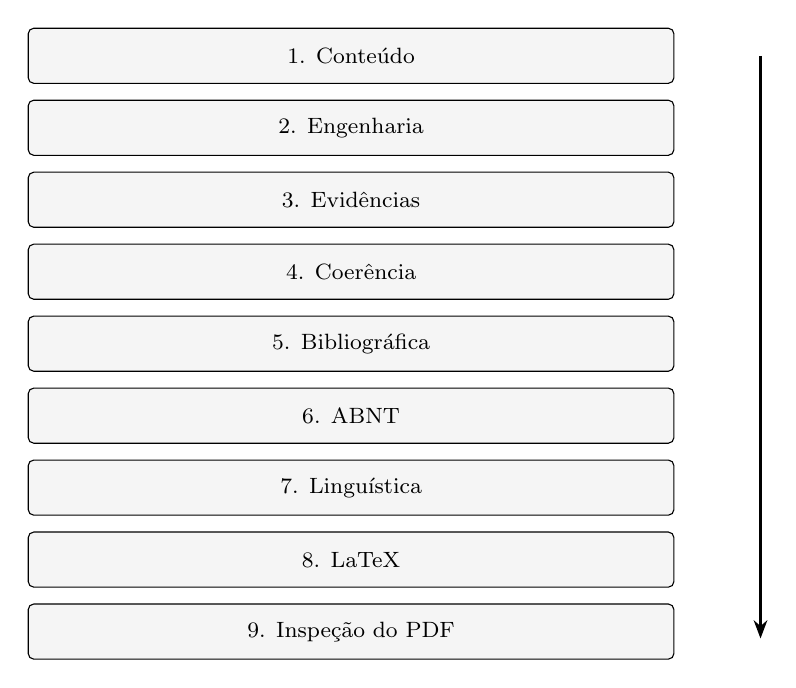
\begin{tikzpicture}[
			font=\footnotesize,
			cam/.style={draw, rounded corners=2pt, minimum width=8.2cm, minimum height=0.7cm, align=center, fill=black!4},
			>=Stealth,
			fl/.style={->, thick}
		]

		\node[cam] (r1) at (0,0) {1. Conteúdo};
		\node[cam, below=0.2cm of r1] (r2) {2. Engenharia};
		\node[cam, below=0.2cm of r2] (r3) {3. Evidências};
		\node[cam, below=0.2cm of r3] (r4) {4. Coerência};
		\node[cam, below=0.2cm of r4] (r5) {5. Bibliográfica};
		\node[cam, below=0.2cm of r5] (r6) {6. ABNT};
		\node[cam, below=0.2cm of r6] (r7) {7. Linguística};
		\node[cam, below=0.2cm of r7] (r8) {8. LaTeX};
		\node[cam, below=0.2cm of r8] (r9) {9. Inspeção do PDF};

		\draw[fl] (5.2,0.0) -- (5.2,-7.4);
	\end{tikzpicture}
	\legend{Fonte: elaborado pelo autor (2026). Neste trabalho, as camadas 1 a 5 foram aplicadas durante a
	produção; a camada 6 foi parcialmente aplicada e depende do manual institucional; as camadas 8 e 9
	\textbf{não foram executadas} por ausência de compilador LaTeX no ambiente --- ver
	\texttt{MONOGRAFIA\_STATUS.md}, seção~3.}
\end{figure}


%% =====================================================================
%%  CAPITULO 3 - TRABALHOS RELACIONADOS
%% =====================================================================

\chapter{Trabalhos Relacionados}
\label{cap:relacionados}

Este capítulo posiciona o trabalho em relação a três linhas: processos
orientados por especificação, agentes de linguagem aplicados ao desenvolvimento
de software e verificação de software assistida por agentes. A comparação é
predominantemente qualitativa; onde uma comparação quantitativa exigiria dados
que não foram consultados na fonte original, isso é declarado.

\section{Processos orientados por especificação}
\label{sec:rel-sdd}

O desenvolvimento orientado por testes estabelece o teste como artefato de
primeira classe, escrito antes da implementação (\citeonline{beck2002tdd}). A
especificação por exemplo leva a ideia adiante, substituindo descrição abstrata
por exemplos concretos que funcionam simultaneamente como requisito, teste e
documentação (\citeonline{adzic2011}). Ambos compartilham o mecanismo central
adotado neste trabalho: o critério de aceitação precede a implementação.

A engenharia de requisitos normatizada fornece o vocabulário para tornar o
critério verificável, incluindo atributos de qualidade de requisito
(\citeonline{iso29148}). O modelo de qualidade de produto
(\citeonline{iso25010}) fornece a taxonomia para classificar requisitos não
funcionais.

O desenvolvimento de linguagens específicas de domínio ilustra o caso extremo da
mesma tese: quando o domínio é bem compreendido, uma notação restrita reduz a
ambiguidade e a possibilidade de erro (\citeonline{mernike2005}). O paralelo com
este trabalho está na função dos identificadores estáveis: ao nomear cada
requisito, critério e tarefa, restringe-se o espaço de referências ambíguas.

\section{Agentes de linguagem no desenvolvimento de software}
\label{sec:rel-agentes}

Três trabalhos representativos organizam múltiplos agentes para produzir software.
MetaGPT atribui papéis análogos aos de uma equipe e representa artefatos
intermediários de forma estruturada, com o argumento de que representações
intermediárias bem definidas reduzem a propagação de erro entre etapas
(\citeonline{hong2024metagpt}). ChatDev modela o desenvolvimento como
conversação entre papéis de projetista, programador e revisor, com foco na
comunicação entre agentes como mecanismo de correção
(\citeonline{qian2024chatdev}). AutoGen trata a conversação entre agentes
configuráveis como primitiva de construção, permitindo compor fluxos com
participação humana (\citeonline{wu2023autogen}).

Esses trabalhos demonstram que a decomposição em papéis melhora a qualidade do
artefato gerado. Entretanto, o critério de sucesso predominante é a qualidade do
código ou a taxa de conclusão da tarefa, e não a existência de uma cadeia
auditável entre requisito, teste e evidência. Em particular, nenhum dos três
define condições de parada por informação ausente como parte do protocolo: o
agente pode continuar produzindo na ausência de dados essenciais.

\section{Padrões de raciocínio e autocorreção}
\label{sec:rel-padroes}

O intercalamento entre raciocínio e ação permite que o agente use o resultado de
uma ação para decidir a próxima, corrigindo a trajetória durante a execução
(\citeonline{yao2023react}). A reflexão sobre o próprio erro, com registro da
avaliação crítica reutilizada em tentativas posteriores, melhora o desempenho em
tarefas que admitem tentativa e erro (\citeonline{shinn2023reflexion}). A
explicitação do raciocínio intermediário melhora o desempenho em tarefas de
múltiplos passos (\citeonline{wei2022}).

Esses padrões são adotados no framework proposto, mas com uma restrição: a
autocorreção é aplicada a artefatos internos (especificação, tarefas, código),
nunca à evidência. A evidência de teste não é objeto de reflexão do agente; ela é
resultado de execução. Essa separação é deliberada e responde ao problema de
opacidade apontado na Seção~\ref{sec:agentes}.

\section{Comparação}
\label{sec:rel-comparacao}

O Quadro~\ref{qua:comparacao} compara os trabalhos segundo cinco critérios
derivados do problema de pesquisa.

\begin{quadro}[htb]
	\caption{Comparação entre abordagens correlatas segundo critérios de controle de processo}
	\label{qua:comparacao}
	\centering
	\footnotesize
	\begin{tabularx}{\textwidth}{@{}p{3.3cm} c c c c c@{}}
		\toprule
		\textbf{Abordagem} &
		\rotatebox{70}{\textbf{Especificação prévia}} &
		\rotatebox{70}{\textbf{Múltiplos papéis}} &
		\rotatebox{70}{\textbf{Critério verificável}} &
		\rotatebox{70}{\textbf{Evidência de execução}} &
		\rotatebox{70}{\textbf{Parada por dado ausente}} \\
		\midrule
		\citeonline{beck2002tdd}      & Parcial & Não  & Sim     & Sim     & Não \\
		\addlinespace
		\citeonline{adzic2011}        & Sim     & Não  & Sim     & Sim     & Não \\
		\addlinespace
		\citeonline{iso29148}         & Sim     & Não  & Sim     & Não     & Não \\
		\addlinespace
		\citeonline{hong2024metagpt}  & Parcial & Sim  & Não     & Não     & Não \\
		\addlinespace
		\citeonline{qian2024chatdev}  & Parcial & Sim  & Não     & Não     & Não \\
		\addlinespace
		\citeonline{wu2023autogen}    & Não     & Sim  & Não     & Parcial & Não \\
		\addlinespace
		\citeonline{yao2023react}     & Não     & Não  & Não     & Sim     & Não \\
		\addlinespace
		\citeonline{shinn2023reflexion} & Não   & Não  & Não     & Sim     & Não \\
		\addlinespace
		\midrule
		\textbf{Processo proposto}    & Sim     & Sim  & Sim     & Sim     & Sim \\
		\bottomrule
	\end{tabularx}
	\legend{Fonte: elaborado pelo autor (2026). A classificação é qualitativa e baseada na leitura
	dos trabalhos; ``parcial'' indica que o critério existe de forma implícita ou incompleta.
	Confirmar cada classificação contra o texto original --- ver P-16 a P-21.}
\end{quadro}

\section{Posicionamento e contribuição pretendida}
\label{sec:rel-posicionamento}

A comparação do Quadro~\ref{qua:comparacao} evidencia que as abordagens existentes
cobrem bem a geração cooperativa e os padrões de raciocínio, mas não combinam, em
um único processo, quatro elementos: especificação prévia obrigatória, critério
verificável com identificador estável, evidência de execução como única fonte de
conclusão e parada explícita diante de informação ausente.

A contribuição pretendida não é um novo modelo de linguagem nem um novo algoritmo
de coordenação. É um \emph{protocolo de controle} aplicável sobre agentes
existentes, com três propriedades verificáveis:

1. \textbf{Rastreabilidade} --- cada entrega é referenciável a um requisito.
2. \textbf{Falseabilidade} --- cada requisito relevante tem um teste capaz de reprová-lo.
3. \textbf{Honestidade epistêmica} --- ausência de dado é registrada como ausência, nunca suprida por estimativa.

A avaliação dessa contribuição é feita por estudo de caso, conforme o
Capítulo~\ref{cap:metodos}, e não por experimento controlado. Essa escolha
metodológica tem custo e benefício, discutidos na Seção~\ref{sec:ameacas}.

%% =====================================================================
%%  CAPITULO 4 - MATERIAIS E METODOS
%% =====================================================================

\chapter{Materiais e Métodos}
\label{cap:metodos}

Este capítulo descreve a natureza da pesquisa, o procedimento, os instrumentos, o
ambiente experimental, as variáveis, as métricas, o tratamento dos dados e as
ameaças à validade. O objetivo é permitir que outro pesquisador avalie
criticamente o trabalho e reproduza o que foi executado.

\section{Natureza e abordagem da pesquisa}
\label{sec:natureza}

A pesquisa é de natureza \textbf{aplicada}, com objetivo \textbf{exploratório e
descritivo}, e abordagem \textbf{qualitativa predominante com componentes
quantitativos pontuais}. O método é o \textbf{estudo de caso único}, adequado
quando o fenômeno é contemporâneo, não manipulável pelo pesquisador e
inseparável do contexto em que ocorre (\citeonline{yin2018}). As diretrizes para
condução e relato de estudos de caso em engenharia de software
(\citeonline{runeson2009}) orientaram a estrutura deste capítulo.

A escolha do estudo de caso em detrimento do experimento controlado é
consequência da pergunta de pesquisa. A pergunta é ``como estruturar um
processo'', e processos são artefatos sócio-técnicos cuja validade depende de
como são operados na prática. Um experimento controlado exigiria um grupo de
controle submetido ao mesmo pedido sem o processo proposto --- o que foi
registrado como dado necessário e não obtido (P-14).

\section{Unidade de análise e contexto}
\label{sec:unidade}

A unidade de análise é a \textbf{execução do processo} sobre um sistema-alvo. O
sistema-alvo é um jogo digital de movimentação em grade, entregue como artefato
único de página web, com os seguintes requisitos de produto declarados na
solicitação original:

\begin{quadro}[htb]
	\caption{Requisitos declarados na solicitação original do produto}
	\label{qua:requisitos-origem}
	\centering
	\footnotesize
	\begin{tabularx}{\textwidth}{@{}c X@{}}
		\toprule
		\textbf{\#} & \textbf{Requisito declarado na solicitação} \\
		\midrule
		R1 & Arquivo único com CSS e JavaScript embutidos na mesma página. \\
		R2 & Ausência de dependências externas: apenas desenho vetorial, CSS e JavaScript nativos. \\
		R3 & Layout moderno, limpo, responsivo e centralizado. \\
		R4 & Tema escuro de estilo retro-arcade com elementos em tons neon. \\
		R5 & Placar com pontuação atual e melhor pontuação persistida no navegador. \\
		R6 & Tela de fim de jogo com botão de reinício. \\
		R7 & Controle por setas do teclado e por teclas W, A, S e D. \\
		R8 & Botões direcionais na tela para uso em dispositivos de toque. \\
		R9 & Bloqueio de inversão instantânea de direção. \\
		R10 & Alvo sorteado em posição aleatória, nunca sobre o corpo do jogador. \\
		R11 & Fim de jogo por colisão com a borda do tabuleiro ou com o próprio corpo. \\
		R12 & Crescimento do jogador e aumento de pontuação a cada alvo consumido. \\
		R13 & Código estruturado, comentado e limpo. \\
		R14 & Laço de jogo eficiente, com \texttt{requestAnimationFrame} ou temporizador controlado. \\
		\bottomrule
	\end{tabularx}
	\legend{Fonte: adaptado de \texttt{docs/memorial.txt} (solicitação original do produto).}
\end{quadro}

\section{Procedimento}
\label{sec:procedimento}

O procedimento teve quatro etapas encadeadas, cada uma produzindo artefatos
consumidos pela seguinte. O pipeline completo está no Quadro~\ref{qua:pipeline}.

\begin{quadro}[htb]
	\caption{Etapas do procedimento e artefatos produzidos}
	\label{qua:pipeline}
	\centering
	\footnotesize
	\begin{tabularx}{\textwidth}{@{}c p{2.6cm} X@{}}
		\toprule
		\textbf{Etapa} & \textbf{Nome} & \textbf{Artefatos produzidos} \\
		\midrule
		E1 & Auditoria e compreensão & Classificação do material disponível; identificação de oito lacunas no material de origem do framework. \\
		\addlinespace
		E2 & Especificação & Especificação com 15 requisitos funcionais, 9 não funcionais, 12 critérios de aceitação, contratos de dados e casos de borda. \\
		\addlinespace
		E3 & Projeto e implementação & Documento com 7 decisões arquiteturais e o artefato de código único. \\
		\addlinespace
		E4 & Verificação & Protocolo de teste, execução das verificações e registro de evidências com resultado por critério. \\
		\bottomrule
	\end{tabularx}
	\legend{Fonte: elaborado pelo autor (2026).}
\end{quadro}

A ordem das etapas não é negociável dentro do processo: a especificação precede a
implementação e a verificação conclui. Essa precedência é a variável independente
do estudo.

\section{Instrumentos}
\label{sec:instrumentos}

Foram usados quatro instrumentos, todos disponíveis no ambiente sem instalação
adicional.

\textbf{Inspeção estática.} Busca textual no artefato para confirmar propriedades
estruturais que não dependem de execução, como a ausência de referências de rede
e a existência de um único bloco de estilo e um único bloco de script.

\textbf{Automação de navegador.} Controle programático de um navegador real para
enviar eventos de teclado e de apontador e para inspecionar o estado observável
da página. Esse instrumento permite verificar comportamento sem instrumentar o
código do produto --- ponto relevante, porque instrumentar o produto para
testá-lo alteraria o objeto de estudo.

\textbf{Leitura de pixels da superfície de desenho.} Amostragem dos pixels do
elemento de desenho para localizar a célula do alvo e a posição da cabeça do
jogador. Essa técnica permitiu implementar um agente de teste que joga o jogo de
forma autônoma, tornando possível verificar crescimento, pontuação e velocidade
sem intervenção manual e sem acesso à estrutura interna do programa.

\textbf{Captura de tela.} Registro visual dos estados de interface, usado como
evidência complementar qualitativa.

\section{Ambiente experimental}
\label{sec:ambiente}

O Quadro~\ref{qua:ambiente} registra o ambiente, conforme exigido para
reprodutibilidade. Os itens marcados como não registrados não foram anotados
durante a execução e não são reconstruídos aqui por estimativa.

\begin{quadro}[htb]
	\caption{Ambiente experimental registrado}
	\label{qua:ambiente}
	\centering
	\footnotesize
	\begin{tabularx}{\textwidth}{@{}p{4.2cm} X@{}}
		\toprule
		\textbf{Item} & \textbf{Registro} \\
		\midrule
		Sistema operacional & Linux \\
		Forma de execução & Arquivo local, protocolo de arquivo, sem servidor \\
		Motor de navegador & Motor Chromium \\
		Versão exata do navegador & [DADO NECESSÁRIO --- não registrado durante a execução] \\
		Resolução da janela & Área de conteúdo de aproximadamente 1200\,px de largura; elemento de desenho com 517,5\,px de lado \\
		Razão de pixels do dispositivo & 1 (não emulado) \\
		Armazenamento local & Disponível e persistente entre recarregamentos \\
		Idioma da interface & Português do Brasil \\
		Preferência de movimento reduzido & [DADO NECESSÁRIO --- estado não registrado] \\
		Duração das sessões de medição & Janela de 150\,s para a medição de velocidade \\
		\bottomrule
	\end{tabularx}
	\legend{Fonte: elaborado pelo autor (2026).}
\end{quadro}

\section{Variáveis}
\label{sec:variaveis}

\textbf{Variável independente:} a presença do processo orientado por
especificação, com critérios de aceitação definidos antes da implementação.

\textbf{Variáveis dependentes:} (i) fração $A$ de critérios de aceitação
satisfeitos, definida na Equação~(\ref{eq:cobertura}); (ii) cobertura de
rastreabilidade, definida como a fração de requisitos com critério de aceitação
associado; (iii) intervalo médio entre passos de simulação, definido na
Equação~(\ref{eq:intervalo-medio}).

\textbf{Variáveis de controle:} as constantes do alvo (dimensões da grade,
intervalo inicial, intervalo mínimo, passo de redução, pontos por item), fixadas
no artefato e registradas na Tabela~\ref{tab:constantes}.

O intervalo entre passos de simulação é o principal alvo de medição quantitativa
porque é a única grandeza de comportamento contínuo cujo valor alvo está declarado
na especificação e que é observável externamente sem instrumentar o produto.

\section{Métricas}
\label{sec:metricas}

A Tabela~\ref{tab:metricas} define as métricas operacionais, a forma de coleta e
a limitação de cada uma.

\begin{table}[htb]
	\caption{Métricas operacionais, coleta e limitação}
	\label{tab:metricas}
	\centering
	\footnotesize
	\begin{tabularx}{\textwidth}{@{}p{2.6cm} X p{3.6cm}@{}}
		\toprule
		\textbf{Métrica} & \textbf{Coleta} & \textbf{Limitação} \\
		\midrule
		$A$ (cobertura de verificação) & Contagem de critérios com resultado observado favorável sobre o total & Mede conformidade com a especificação, não adequação ao uso \\
		\addlinespace
		Rastreabilidade de requisitos & Contagem de requisitos com critério de aceitação associado sobre o total & Não avalia a qualidade do critério, apenas sua existência \\
		\addlinespace
		$t$ (intervalo entre passos) & Marcações de tempo do observador entre mudanças sucessivas da posição da cabeça & A granularidade do observador adiciona erro positivo; o valor medido é um limite superior \\
		\addlinespace
		Comprimento do jogador & Contagem de células ocupadas na superfície de desenho & Depende da detecção correta de cor \\
		\addlinespace
		Colisões indevidas & Contagem de amostras em que o alvo coincidiu com célula do corpo & Limitada ao número de amostras coletadas \\
		\bottomrule
	\end{tabularx}
	\legend{Fonte: elaborado pelo autor (2026).}
\end{table}

O erro positivo do observador na medição de $t$ merece destaque, porque justifica
o tratamento adotado. Seja $\varepsilon$ o atraso introduzido pelo ciclo de
observação. O intervalo medido é $t_{\mathrm{med}} = t_{\mathrm{real}} +
\varepsilon$. Como $\varepsilon$ é aproximadamente constante ao longo de uma
janela, a comparação entre janelas preserva a \emph{diferença} mas não o valor
absoluto. Por isso, os valores absolutos medidos não são tratados como
estimativas do parâmetro do alvo; o que se afirma é a \emph{ordem} e a
\emph{direção} da variação, conforme a Equação~(\ref{eq:intervalo-medio}).

\section{Tratamento dos dados}
\label{sec:tratamento}

Para cada mudança de posição da cabeça do jogador registrou-se um par
(instante, pontuação corrente). O intervalo médio entre passos em uma faixa de
pontuação foi estimado por:

\begin{equation}
	\mathrm{E}[T] \;=\; \frac{1}{m-1}
	\sum_{i=2}^{m} \left( \tau_i - \tau_{i-1} \right)
	\label{eq:intervalo-medio}
\end{equation}

\noindent em que $\tau_i$ é o instante da $i$-ésima mudança de posição e $m$ é o
número de mudanças observadas na faixa. A média, e não a mediana, foi adotada
como tratamento principal porque o erro de observação $\varepsilon$ é aditivo e
aproximadamente constante: a média o absorve de forma previsível, enquanto a
mediana o distribui de modo dependente da amostra.

A estatística descritiva completa por faixa --- contagem, média, mínimo e máximo
--- está reportada no Capítulo~\ref{cap:resultados}. Não se aplicou teste de
hipótese, pelo tamanho da amostra e pela natureza de estudo de caso; essa escolha
é retomada em \ref{sec:ameacas}.

\section{Ética e integridade}
\label{sec:etica}

O trabalho não envolveu seres humanos como sujeitos de pesquisa, não coletou
dados pessoais e não utiliza dados sensíveis; a apreciação por comitê de ética
não se aplica. O produto armazena apenas um valor numérico de recorde no
armazenamento local do navegador de quem o executa.

Declara-se explicitamente a política de integridade adotada: nenhum dado,
medição, resultado ou referência foi estimado, interpolado ou produzido de
memória. Informação ausente recebeu marcador explícito e foi registrada em
\texttt{MONOGRAFIA\_PENDENCIAS.md}. As referências bibliográficas foram
declaradas sem identificadores não verificados --- sem ISBN ou DOI inventados
--- e exigem conferência contra a fonte original antes da entrega final.

\section{Ameaças à validade}
\label{sec:ameacas}

A classificação segue \citeonline{wohlin2012} e \citeonline{runeson2009}. O
Quadro~\ref{qua:ameacas} enumera as ameaças identificadas, a categoria e a
mitigação efetivamente aplicada.

\begin{quadro}[htb]
	\caption{Ameaças à validade identificadas e mitigações}
	\label{qua:ameacas}
	\centering
	\footnotesize
	\begin{tabularx}{\textwidth}{@{}c p{4.6cm} X@{}}
		\toprule
		\textbf{ID} & \textbf{Ameaça} & \textbf{Categoria e mitigação} \\
		\midrule
		AV-1 & Ausência de grupo de controle que executou o mesmo alvo sem o processo proposto & \textit{Validade interna}. Não mitigada. Sem controle não é possível atribuir o resultado ao processo em vez de à competência do executor ou à simplicidade do alvo. Mitigação parcial: registrar a lacuna (P-14). \\
		\addlinespace
		AV-2 & Estudo de caso único em um domínio com estado discreto e regras bem definidas & \textit{Validade externa}. Generalização limitada a domínios de complexidade comparável. Mitigação: declarar explicitamente o escopo de generalização. \\
		\addlinespace
		AV-3 & Autoria do executante e do observador coincidirem & \textit{Validade de construto}. Risco de confirmação. Mitigação: a evidência é produzida por execução automatizada e por inspeção textual reproduzível, não por julgamento do autor. \\
		\addlinespace
		AV-4 & A métrica de rastreabilidade avalia existência de critério, não sua qualidade & \textit{Validade de construto}. Um critério mal formulado contaria como cobertura. Mitigação: não mitigada; registrada como limitação da métrica. \\
		\addlinespace
		AV-5 & Erro positivo na medição do intervalo por ciclo de observação & \textit{Validade de conclusão}. Afeta valores absolutos. Mitigação: reportar apenas a direção da variação e declarar o viés. \\
		\addlinespace
		AV-6 & Amostra temporal única por faixa, sem repetição nem intervalo de confiança & \textit{Validade de conclusão}. Não permite inferência estatística. Mitigação: não mitigada; repetição registrada como dado necessário (P-11). \\
		\addlinespace
		AV-7 & Detecção de posições por cor, sujeita a erro em pixels de borda & \textit{Validade de construto}. Mitigação: critérios de cor restritivos e verificação de que a célula do alvo nunca foi classificada como corpo em 25 amostras. \\
		\bottomrule
	\end{tabularx}
	\legend{Fonte: elaborado pelo autor (2026), a partir de \citeonline{wohlin2012} e \citeonline{runeson2009}.}
\end{quadro}

Duas ameaças não foram mitigadas: a ausência de grupo de controle (AV-1) e a
ausência de repetição com tratamento estatístico (AV-6). Ambas exigiriam trabalho
experimental adicional. Registrá-las explicitamente é preferível a apresentar os
resultados como se essas limitações não existissem.

%% =====================================================================
%%  CAPITULO 5 - O FRAMEWORK SDD AGENTICO
%% =====================================================================

\chapter{O Framework SDD Agêntico}
\label{cap:framework}

Este capítulo descreve o processo proposto: sua arquitetura, os agentes, as
instruções permanentes, as habilidades de domínio, o fluxo adaptativo, os portões
de verificação, a definição de concluído, o protocolo de contexto e as condições
de parada. O framework é a variável independente do estudo.

\section{Princípios de projeto}
\label{sec:fw-principios}

O framework foi projetado a partir de oito princípios operacionais, adotados como
regras de conduta do executor:

\begin{enumerate}
	\item Planejar antes de editar.
	\item Verificar antes de assumir.
	\item Implementar pouco por vez.
	\item Testar imediatamente.
	\item Registrar decisões importantes.
	\item Nunca esconder incerteza.
	\item Nunca fabricar evidência.
	\item Nunca declarar validação física sem validação física.
\end{enumerate}

Os princípios 6 a 8 são os mais consequentes para o resultado deste trabalho.
Eles convertem uma postura epistemológica em regra operacional: a ausência de
dado não é uma falha a ser disfarçada, mas um estado a ser declarado. O item 8 é
específico ao domínio de sistemas embarcados do material de origem e estabelece
que nenhum nível de evidência pode ser promovido por analogia --- teste em
simulador não promove um resultado a validado em bancada.

\section{Motivação: lacunas do material de origem}
\label{sec:fw-lacunas}

O ponto de partida foi uma avaliação crítica de um conjunto prévio de artefatos
de processo. Essa avaliação identificou oito oportunidades de melhoria, listadas
no Quadro~\ref{qua:lacunas} com o tratamento dado a cada uma no framework
proposto.

\begin{quadro}[htb]
	\caption{Lacunas identificadas no material de origem e tratamento no framework}
	\label{qua:lacunas}
	\centering
	\footnotesize
	\begin{tabularx}{\textwidth}{@{}c p{5.4cm} X@{}}
		\toprule
		\textbf{\#} & \textbf{Lacuna identificada} & \textbf{Tratamento no framework proposto} \\
		\midrule
		L1 & Fluxo linear demais, com cadeia completa mesmo para alterações pequenas & Roteamento por complexidade e risco, com quatro trilhas (Seção~\ref{sec:fw-fluxo}) \\
		\addlinespace
		L2 & Ausência de um portão independente de verificação & Agente dedicado a responder se há evidência suficiente para declarar conclusão \\
		\addlinespace
		L3 & Economia de contexto não era regra operacional permanente & Conjunto de instruções permanentes com dez regras de contexto \\
		\addlinespace
		L4 & Falta de separação explícita entre estado real e memória da conversa & Protocolo de contexto com ordem de precedência de fontes \\
		\addlinespace
		L5 & Rastreabilidade definida em conceito, não operacionalizada & Matriz de rastreabilidade com formato fixo e regra de evidência obrigatória \\
		\addlinespace
		L6 & Risco de duplicação entre documentos de estado e de transferência & Definição de papel único por documento; transferência só quando há continuidade \\
		\addlinespace
		L7 & Ausência de mecanismo explícito de parada & Seis condições de parada obrigatórias \\
		\addlinespace
		L8 & Definição de concluído dispersa em vários documentos & Lista única de verificação de encerramento com quatorze itens \\
		\bottomrule
	\end{tabularx}
	\legend{Fonte: elaborado pelo autor (2026) a partir da avaliação crítica do material de origem.}
\end{quadro}

\section{Arquitetura em camadas}
\label{sec:fw-camadas}

O framework organiza-se em cinco camadas com responsabilidades distintas, como
ilustra a Figura~\ref{fig:camadas}. A separação é funcional: cada camada responde
a uma pergunta diferente, e a violação da fronteira entre camadas é a origem mais
comum de degradação de processo.

%% ---------------------------------------------------------------------
%%  FIGURA - Camadas do framework proposto (DG-02)
%% ---------------------------------------------------------------------
\begin{figure}[htb]
	\caption{Camadas do framework SDD agêntico e responsabilidade de cada uma}
	\label{fig:camadas}
	\centering
	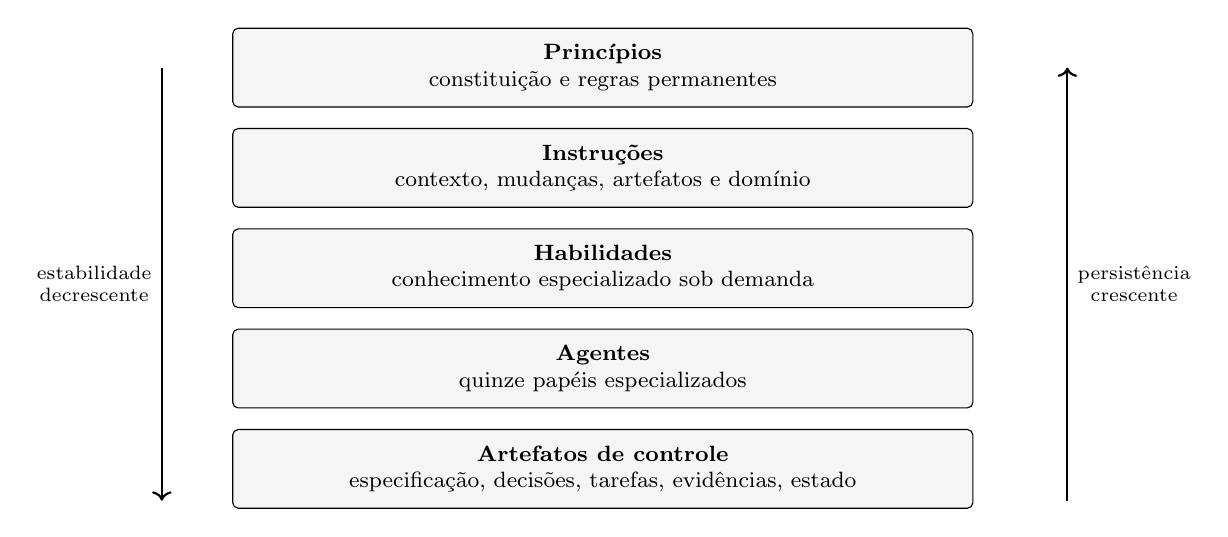
\begin{tikzpicture}[
			font=\footnotesize,
			camada/.style={
					draw,
					rounded corners=2pt,
					minimum width=9.4cm,
					minimum height=1.0cm,
					align=center,
					fill=black!4
				}
		]
		\node[camada] (c1) at (0,0) {\textbf{Princípios}\\ constituição e regras permanentes};
		\node[camada, below=0.26cm of c1] (c2) {\textbf{Instruções}\\ contexto, mudanças, artefatos e domínio};
		\node[camada, below=0.26cm of c2] (c3) {\textbf{Habilidades}\\ conhecimento especializado sob demanda};
		\node[camada, below=0.26cm of c3] (c4) {\textbf{Agentes}\\ quinze papéis especializados};
		\node[camada, below=0.26cm of c4] (c5) {\textbf{Artefatos de controle}\\ especificação, decisões, tarefas, evidências, estado};

		\draw[->, thick] (-5.6,0.0) -- (-5.6,-5.5)
		node[midway, left, align=center, font=\scriptsize] {estabilidade\\ decrescente};
		\draw[->, thick] (5.9,-5.5) -- (5.9,0.0)
		node[midway, right, align=center, font=\scriptsize] {persistência\\ crescente};
	\end{tikzpicture}
	\legend{Fonte: elaborado pelo autor (2026) a partir da estrutura do repositório.}
\end{figure}


\textbf{Camada de princípios.} Contém o que não muda com a tarefa: a constituição
e as regras permanentes. É a camada mais estável e a de maior precedência.

\textbf{Camada de instruções.} Contém regras operacionais de aplicação ampla:
economia de contexto, controle de mudanças, artefatos e engenharia de domínio.
Instruções são carregadas por padrão de arquivo afetado, e não por decisão
discricionária.

\textbf{Camada de habilidades.} Contém conhecimento de domínio acionado sob
demanda: produção de especificação, desenvolvimento embarcado, artigo científico,
monografia e documentação de projeto. Habilidades não são carregadas
preventivamente.

\textbf{Camada de agentes.} Contém quinze papéis especializados, cada um com
entrada esperada, artefatos que pode ler, artefatos que pode alterar e portão de
saída.

\textbf{Camada de artefatos de controle.} Contém o estado do trabalho:
especificação, decisões, tarefas, estado, transferência e matriz de
rastreabilidade. É a única camada que persiste entre sessões.

\section{Agentes}
\label{sec:fw-agentes}

Os quinze agentes distribuem-se em quatro grupos funcionais, conforme o
Quadro~\ref{qua:agentes}.

\begin{quadro}[htb]
	\caption{Agentes do framework, por grupo funcional}
	\label{qua:agentes}
	\centering
	\footnotesize
	\begin{tabularx}{\textwidth}{@{}c p{3.4cm} X@{}}
		\toprule
		\textbf{\#} & \textbf{Agente} & \textbf{Responsabilidade} \\
		\midrule
		\multicolumn{3}{@{}l}{\textit{Grupo A --- Roteamento e planejamento}} \\
		\midrule
		00 & \texttt{task-router} & Classifica a solicitação, estima complexidade e risco e encaminha ao menor fluxo suficiente \\
		\addlinespace
		01 & \texttt{product-planner} & Define escopo, objetivos, restrições, riscos e critérios de sucesso \\
		\addlinespace
		02 & \texttt{requirements-engineer} & Redige requisitos funcionais e não funcionais, regras de negócio, casos de uso e critérios de aceitação \\
		\addlinespace
		03 & \texttt{architect} & Define componentes, interfaces, dados, tecnologias e decisões arquiteturais \\
		\addlinespace
		04 & \texttt{task-planner} & Decompõe requisitos e arquitetura em tarefas pequenas, ordenadas e verificáveis \\
		\midrule
		\multicolumn{3}{@{}l}{\textit{Grupo B --- Execução}} \\
		\midrule
		05 & \texttt{implementer} & Executa a tarefa aprovada seguindo requisitos, arquitetura e padrões do projeto \\
		\midrule
		\multicolumn{3}{@{}l}{\textit{Grupo C --- Verificação}} \\
		\midrule
		06 & \texttt{code-reviewer} & Avalia corretude, qualidade, manutenibilidade, testes e aderência à arquitetura \\
		\addlinespace
		07 & \texttt{test-engineer} & Define a estratégia de teste e cria testes de unidade, integração, sistema e ponta a ponta \\
		\addlinespace
		08 & \texttt{security-reviewer} & Avalia risco em código, arquitetura, dependências, configuração e tratamento de dados \\
		\addlinespace
		13 & \texttt{verification-gate} & Responde se há evidência suficiente para declarar a tarefa concluída \\
		\midrule
		\multicolumn{3}{@{}l}{\textit{Grupo D --- Encerramento e continuidade}} \\
		\midrule
		09 & \texttt{documentation} & Mantém a documentação técnica e de uso sincronizada \\
		\addlinespace
		10 & \texttt{integration-agent} & Valida a integração entre módulos, serviços, hardware e interfaces \\
		\addlinespace
		11 & \texttt{release-agent} & Verifica qualidade, documentação, versionamento e critérios de aceite antes da liberação \\
		\addlinespace
		12 & \texttt{project-orchestrator} & Coordena os demais agentes e preserva a rastreabilidade do roteamento à transferência \\
		\addlinespace
		14 & \texttt{handoff-manager} & Produz transferência compacta e verificável entre agentes ou sessões \\
		\bottomrule
	\end{tabularx}
	\legend{Fonte: elaborado pelo autor (2026) a partir de \texttt{.github/agents/}.}
\end{quadro}

A separação entre o agente que implementa (05) e os que verificam (06, 07, 13) é
deliberada e corresponde ao princípio clássico de independência entre construção e
verificação. O agente \texttt{code-reviewer} e o \texttt{test-engineer} avaliam;
o \texttt{verification-gate} decide. Concentrar as três funções em um único papel
reproduziria o problema que a separação pretende resolver.

\section{Instruções permanentes}
\label{sec:fw-instrucoes}

Quatro conjuntos de instruções são aplicados por padrão de arquivo afetado. Essa
forma de aplicação --- automática e baseada em caminho --- remove a decisão de
carregar ou não carregar da esfera discricionária do executor, o que é relevante
quando o executor é um agente.

\begin{quadro}[htb]
	\caption{Instruções permanentes do framework}
	\label{qua:instrucoes}
	\centering
	\footnotesize
	\begin{tabularx}{\textwidth}{@{}p{4.2cm} p{2.6cm} X@{}}
		\toprule
		\textbf{Instrução} & \textbf{Aplicação} & \textbf{Conteúdo} \\
		\midrule
		Economia de contexto & Todos os arquivos & Dez regras de inspeção incremental; proíbe varredura proativa; obriga leitura de estado antes de alterar \\
		\addlinespace
		Engenharia embarcada & Código C, C++, Rust, Python e assembly & Restrições de memória, tempo real, concorrência e segurança específicas do domínio \\
		\addlinespace
		Artefatos SDD & Especificações, documentação e arquivos de estado & Convenções de identificador (\texttt{FR}, \texttt{NFR}, \texttt{CA}, \texttt{T}, \texttt{ADR}) e regra de evidência obrigatória \\
		\addlinespace
		Controle de mudanças & Todos os arquivos & Escopo, menor alteração suficiente, proibição de alterar testes para fazê-los passar e verificação posterior obrigatória \\
		\bottomrule
	\end{tabularx}
	\legend{Fonte: elaborado pelo autor (2026) a partir de \texttt{.github/instructions/}.}
\end{quadro}

A instrução de controle de mudanças contém uma proibição que merece destaque:
é vedado alterar testes com o objetivo de fazê-los passar. Essa é a regra que
impede a degradação mais comum de processos de verificação --- a adaptação
retroativa do critério ao resultado obtido.

\section{Habilidades de domínio}
\label{sec:fw-skills}

Cinco habilidades concentram conhecimento especializado, carregado apenas quando a
tarefa correspondente está ativa:

\begin{itemize}
	\item \textbf{Criação de especificação} --- estrutura de especificação otimizada para consumo por agente, com distinção entre requisito, restrição e recomendação.
	\item \textbf{Desenvolvimento embarcado} --- especificação e implementação de firmware, com níveis de evidência e fluxo adaptativo.
	\item \textbf{Artigo científico em LaTeX} --- produção com rigor metodológico e referências verificáveis.
	\item \textbf{Monografia de engenharia em LaTeX} --- produção com conformidade ABNT, diagramas e projeto compilável.
	\item \textbf{Documentação de projeto} --- criação e manutenção do arquivo de apresentação do repositório.
\end{itemize}

O carregamento sob demanda é o mecanismo que resolve a tensão identificada na
Seção~\ref{sec:contexto-custo}: conhecimento especializado existe sem ocupar
contexto quando não é necessário.

\section{Fluxo adaptativo}
\label{sec:fw-fluxo}

O fluxo não aplica a cadeia completa a toda solicitação. O roteador classifica a
complexidade e o risco e seleciona a trilha mínima suficiente, como ilustra a
Figura~\ref{fig:fluxo-agentico}. Essa decisão responde diretamente à lacuna L1.

%% ---------------------------------------------------------------------
%%  FIGURA - Fluxo agentico adaptativo por complexidade (DG-01)
%% ---------------------------------------------------------------------
\begin{figure}[htb]
	\caption{Fluxo agêntico adaptativo: classificação por complexidade e risco}
	\label{fig:fluxo-agentico}
	\centering
	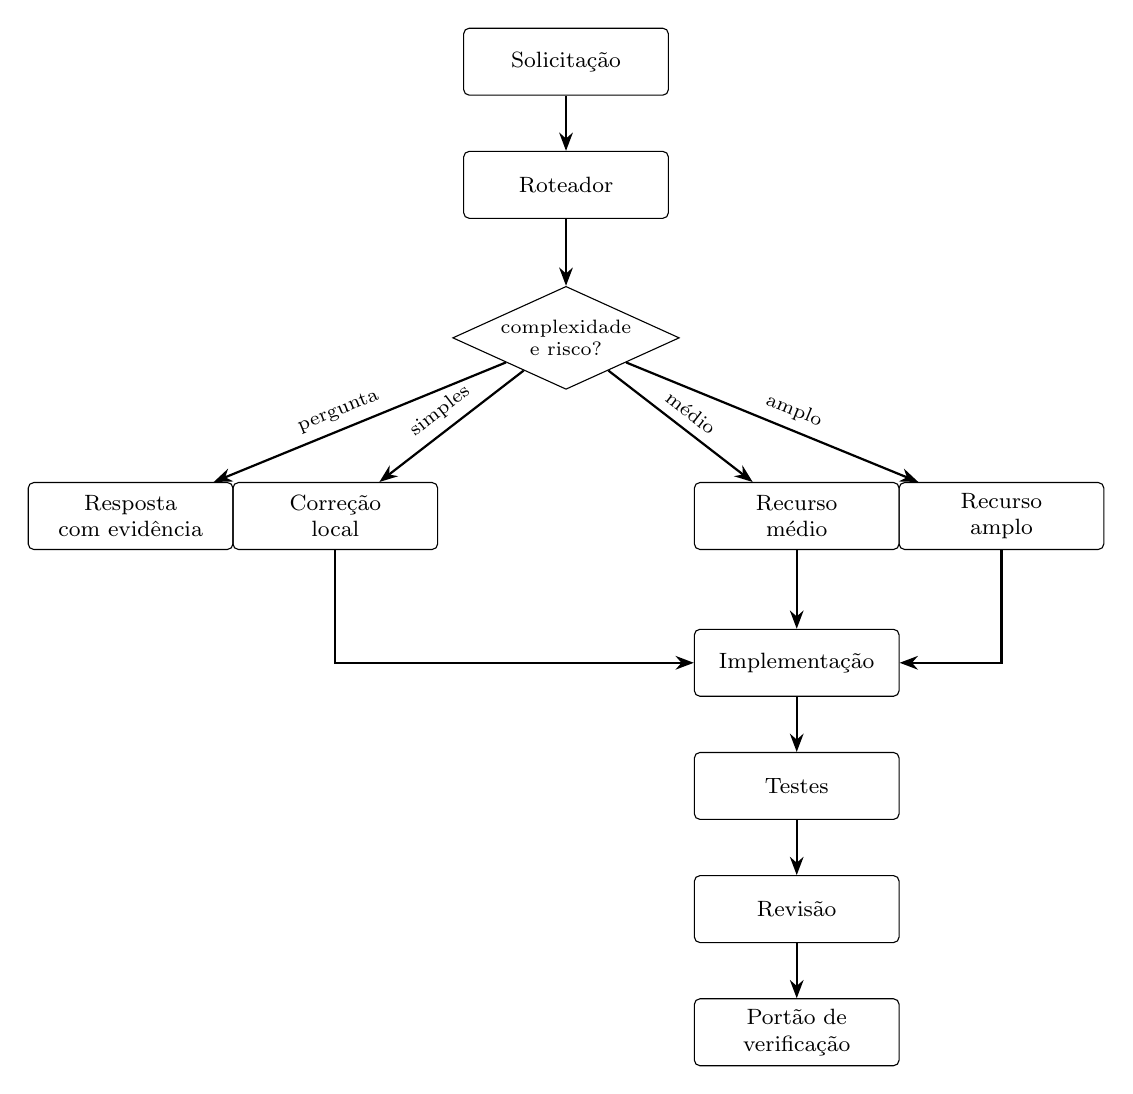
\begin{tikzpicture}[
			font=\footnotesize,
			no/.style={draw, rounded corners=2pt, minimum width=2.6cm, minimum height=0.85cm, align=center},
			dec/.style={draw, diamond, aspect=2.2, inner sep=1pt, align=center, font=\scriptsize},
			>=Stealth,
			fl/.style={->, thick}
		]

		\node[no] (req) at (0,0) {Solicitação};
		\node[no, below=0.7cm of req] (router) {Roteador};
		\node[dec, below=0.85cm of router] (risco) {complexidade\\ e risco?};

		\node[no, below left=1.5cm and 3.5cm of risco] (resp) {Resposta\\ com evidência};
		\node[no, below left=1.5cm and 0.9cm of risco] (quick) {Correção\\ local};
		\node[no, below right=1.5cm and 0.9cm of risco] (medio) {Recurso\\ médio};
		\node[no, below right=1.5cm and 3.5cm of risco] (grande) {Recurso\\ amplo};

		\draw[fl] (req) -- (router);
		\draw[fl] (router) -- (risco);
		\draw[fl] (risco) -- node[sloped, above, font=\scriptsize, pos=0.55] {pergunta} (resp);
		\draw[fl] (risco) -- node[sloped, above, font=\scriptsize] {simples} (quick);
		\draw[fl] (risco) -- node[sloped, above, font=\scriptsize] {médio} (medio);
		\draw[fl] (risco) -- node[sloped, above, font=\scriptsize, pos=0.55] {amplo} (grande);

		\node[no, below=1.0cm of medio] (impl) {Implementação};
		\draw[fl] (quick) |- (impl);
		\draw[fl] (medio) -- (impl);
		\draw[fl] (grande) |- (impl);

		\node[no, below=0.7cm of impl] (teste) {Testes};
		\node[no, below=0.7cm of teste] (revisao) {Revisão};
		\node[no, below=0.7cm of revisao] (gate) {Portão de\\ verificação};

		\draw[fl] (impl) -- (teste);
		\draw[fl] (teste) -- (revisao);
		\draw[fl] (revisao) -- (gate);
	\end{tikzpicture}
	\legend{Fonte: elaborado pelo autor (2026) a partir de \texttt{docs/agentic/WORKFLOW.md}.
	A trilha de liberação, aplicada após o portão de verificação, foi omitida para preservar a legibilidade.}
\end{figure}


O Quadro~\ref{qua:trilhas} descreve as quatro trilhas e o critério de elevação
entre elas.

\begin{quadro}[htb]
	\caption{Trilhas do fluxo adaptativo e critério de elevação}
	\label{qua:trilhas}
	\centering
	\footnotesize
	\begin{tabularx}{\textwidth}{@{}p{2.2cm} X p{3.4cm}@{}}
		\toprule
		\textbf{Trilha} & \textbf{Sequência de agentes} & \textbf{Critério de elevação} \\
		\midrule
		Pergunta & Resposta fundamentada, sem alteração de artefato & Necessidade de alterar qualquer arquivo \\
		\addlinespace
		Correção local & Roteador, executor, portão de verificação & Alteração de comportamento observável \\
		\addlinespace
		Recurso médio & Roteador, requisitos, executor, teste, revisão, verificação & Necessidade de decisão arquitetural \\
		\addlinespace
		Recurso amplo & Planejamento, requisitos, arquitetura, tarefas, execução, teste, revisão, segurança, verificação, documentação, integração & --- \\
		\addlinespace
		Liberação & Verificação, segurança, documentação, integração, liberação & --- \\
		\bottomrule
	\end{tabularx}
	\legend{Fonte: elaborado pelo autor (2026).}
\end{quadro}

\section{Portões de verificação}
\label{sec:fw-gates}

Seis portões pontuam o fluxo, conforme a Figura~\ref{fig:pipeline-gates} e o
Quadro~\ref{qua:gates}.

%% ---------------------------------------------------------------------
%%  FIGURA - Pipeline SDD com portoes de verificacao (DG-03)
%% ---------------------------------------------------------------------
\begin{figure}[htb]
	\caption{Pipeline SDD com os seis portões de verificação}
	\label{fig:pipeline-gates}
	\centering
	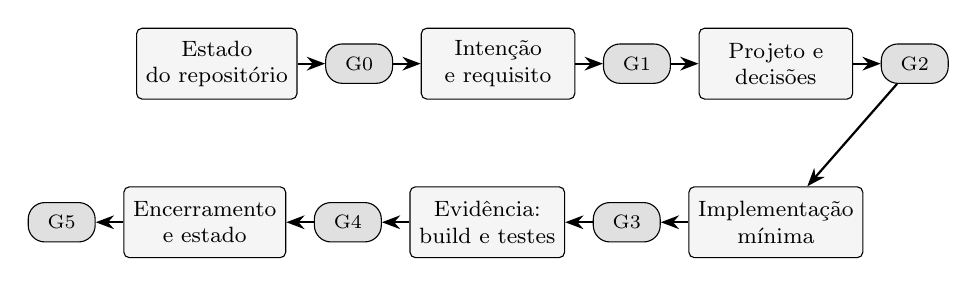
\begin{tikzpicture}[
			font=\footnotesize,
			etapa/.style={draw, rounded corners=2pt, minimum width=1.95cm, minimum height=0.9cm, align=center, fill=black!4},
			portao/.style={draw, fill=black!12, rounded corners=6pt, minimum width=0.85cm, minimum height=0.5cm, font=\scriptsize, align=center},
			>=Stealth,
			fl/.style={->, thick}
		]

		\node[etapa] (e1) at (0,0) {Estado\\ do repositório};
		\node[portao, right=0.35cm of e1] (g0) {G0};
		\node[etapa, right=0.35cm of g0] (e2) {Intenção\\ e requisito};
		\node[portao, right=0.35cm of e2] (g1) {G1};
		\node[etapa, right=0.35cm of g1] (e3) {Projeto e\\ decisões};
		\node[portao, right=0.35cm of e3] (g2) {G2};
		\node[etapa, below=1.1cm of e3] (e4) {Implementação\\ mínima};
		\node[portao, left=0.35cm of e4] (g3) {G3};
		\node[etapa, left=0.35cm of g3] (e5) {Evidência:\\ build e testes};
		\node[portao, left=0.35cm of e5] (g4) {G4};
		\node[etapa, left=0.35cm of g4] (e6) {Encerramento\\ e estado};
		\node[portao, left=0.35cm of e6] (g5) {G5};

		\draw[fl] (e1) -- (g0);
		\draw[fl] (g0) -- (e2);
		\draw[fl] (e2) -- (g1);
		\draw[fl] (g1) -- (e3);
		\draw[fl] (e3) -- (g2);
		\draw[fl] (g2) -- (e4);
		\draw[fl] (e4) -- (g3);
		\draw[fl] (g3) -- (e5);
		\draw[fl] (e5) -- (g4);
		\draw[fl] (g4) -- (e6);
		\draw[fl] (e6) -- (g5);
	\end{tikzpicture}
	\legend{Fonte: elaborado pelo autor (2026) a partir de \texttt{docs/agentic/WORKFLOW.md}.
	O portão G2 é aplicado apenas quando a complexidade exige decisão arquitetural.}
\end{figure}


\begin{quadro}[htb]
	\caption{Portões de verificação do framework}
	\label{qua:gates}
	\centering
	\footnotesize
	\begin{tabularx}{\textwidth}{@{}c p{3.2cm} X@{}}
		\toprule
		\textbf{Portão} & \textbf{Nome} & \textbf{Condição de passagem} \\
		\midrule
		G0 & Estado & Estado real do repositório inspecionado antes de qualquer alteração \\
		\addlinespace
		G1 & Intenção & Requisito e critério de aceitação identificados \\
		\addlinespace
		G2 & Projeto & Decisão arquitetural registrada quando a complexidade exige \\
		\addlinespace
		G3 & Implementação & Alteração mínima, rastreável e restrita ao escopo \\
		\addlinespace
		G4 & Evidência & Compilação, testes e validações aplicáveis executados \\
		\addlinespace
		G5 & Encerramento & Documentação, rastreabilidade, estado e riscos atualizados \\
		\bottomrule
	\end{tabularx}
	\legend{Fonte: elaborado pelo autor (2026) a partir de \texttt{docs/agentic/WORKFLOW.md}.}
\end{quadro}

O portão G1 é o que garante a precedência do critério sobre a implementação: sem
requisito e critério identificados, o fluxo não avança para a execução. O portão
G4 é o que impede a conclusão sem evidência.

\section{Definição de concluído}
\label{sec:fw-dod}

A definição de concluído consolida, em uma única lista de quatorze itens, o que
estava disperso em vários documentos de origem (lacuna L8):

1.~requisito relacionado identificado; 2.~critérios de aceitação verificados;
3.~estado do repositório inspecionado antes da alteração; 4.~alteração no menor
escopo necessário; 5.~compilação do alvo executada; 6.~testes executados;
7.~análise estática executada quando aplicável; 8.~consumo de memória e tempo
verificados quando aplicável; 9.~documentação atualizada; 10.~rastreabilidade
atualizada; 11.~arquivo de estado atualizado se houve mudança significativa;
12.~arquivo de transferência atualizado apenas se houver continuidade;
13.~riscos residuais registrados; 14.~nenhuma alteração não relacionada
incorporada.

Os itens 5, 6, 7 e 8 são ``quando aplicável''. Essa qualificação é deliberada: em
um artefato sem compilação --- como o produto deste estudo de caso, que é
interpretado diretamente pelo navegador --- não existe etapa de compilação, e
exigi-la produziria um item permanentemente não cumprido. A condição de
aplicabilidade precisa ser declarada, e não presumida.

\section{Protocolo de contexto}
\label{sec:fw-contexto}

O protocolo de contexto estabelece a ordem de precedência entre fontes de
informação:

\begin{enumerate}
	\item estado real do repositório e do sistema de controle de versão;
	\item princípios permanentes;
	\item especificação do recurso;
	\item registro de decisões arquiteturais;
	\item tarefas;
	\item código atual;
	\item testes e evidências;
	\item arquivos de estado e de transferência;
	\item histórico da conversa.
\end{enumerate}

A regra central é: \emph{o histórico da conversa pode fornecer intenção, mas nunca
deve substituir a leitura do estado atual do repositório}. Essa regra endereça a
lacuna L4 e é a defesa direta contra a falha mais insidiosa em fluxos executados
por agentes --- tratar uma versão lembrada de um arquivo como se fosse a versão
presente. A posição do histórico no último nível da hierarquia é a expressão
formal dessa defesa.

\section{Condições de parada}
\label{sec:fw-parada}

Seis condições obrigam a interrupção do fluxo e o pedido de decisão, em vez de
prosseguimento sob suposição:

\begin{enumerate}
	\item informação essencial de hardware ausente;
	\item duas especificações em conflito;
	\item necessidade de mudança arquitetural não aprovada;
	\item risco de perda de dados ou de persistência;
	\item impacto de segurança não especificado;
	\item teste obrigatório que não pode ser executado quando o resultado é necessário para liberar a tarefa.
\end{enumerate}

A segunda condição é a que produz mais consequências neste trabalho, porque uma
situação dessa natureza foi de fato encontrada: o repositório descreve um sistema
embarcado e contém, simultaneamente, um produto de página web. Diante do conflito,
a conduta adotada foi registrar a divergência e declarar a escolha, em vez de
produzir documentação sobre um sistema que não existe no repositório
(Seção~\ref{sec:delimitacao}).

\section{Matriz de rastreabilidade}
\label{sec:fw-rastreabilidade}

A matriz operacionaliza a rastreabilidade (lacuna L5) com sete colunas fixas:
requisito, critério, tarefa, código, teste, evidência e estado. Três regras a
governam: não marcar como aprovado sem evidência; acompanhar toda pendência de
justificativa e risco residual; e propagar toda alteração de requisito para
tarefa, teste e documentação.

Figura~\ref{fig:rastreabilidade} representa a cadeia de rastreabilidade aplicada
ao estudo de caso.

%% ---------------------------------------------------------------------
%%  FIGURA - Cadeia de rastreabilidade requisito-evidencia (DG-09)
%% ---------------------------------------------------------------------
\begin{figure}[htb]
	\caption{Cadeia de rastreabilidade do requisito à evidência}
	\label{fig:rastreabilidade}
	\centering
	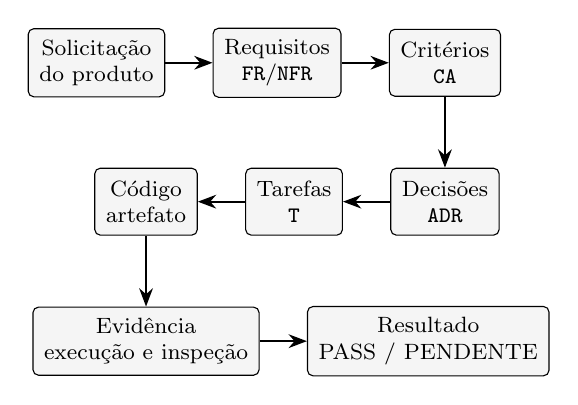
\begin{tikzpicture}[
			font=\footnotesize,
			caixa/.style={draw, rounded corners=2pt, minimum height=0.85cm, align=center, fill=black!4, inner sep=4pt},
			>=Stealth,
			fl/.style={->, thick}
		]

		\node[caixa] (mem) at (0,0) {Solicitação\\ do produto};
		\node[caixa, right=0.6cm of mem] (req) {Requisitos\\ \texttt{FR}/\texttt{NFR}};
		\node[caixa, right=0.6cm of req] (ca) {Critérios\\ \texttt{CA}};
		\node[caixa, below=0.9cm of ca] (adr) {Decisões\\ \texttt{ADR}};
		\node[caixa, left=0.6cm of adr] (tar) {Tarefas\\ \texttt{T}};
		\node[caixa, left=0.6cm of tar] (cod) {Código\\ artefato};
		\node[caixa, below=0.9cm of cod] (evd) {Evidência\\ execução e inspeção};
		\node[caixa, right=0.6cm of evd] (res) {Resultado\\ PASS / PENDENTE};

		\draw[fl] (mem) -- (req);
		\draw[fl] (req) -- (ca);
		\draw[fl] (ca) -- (adr);
		\draw[fl] (adr) -- (tar);
		\draw[fl] (tar) -- (cod);
		\draw[fl] (cod) -- (evd);
		\draw[fl] (evd) -- (res);
	\end{tikzpicture}
	\legend{Fonte: elaborado pelo autor (2026). A ausência de critério rompe a cadeia entre requisito e
	evidência: é exatamente o caso dos dez requisitos marcados como \textbf{SEM CA} no Apêndice~\ref{ap:rastreabilidade}.}
\end{figure}


\section{Síntese do capítulo}
\label{sec:fw-sintese}

O framework proposto é um protocolo de controle: cinco camadas, quinze agentes,
quatro conjuntos de instruções, cinco habilidades, seis portões, catorze itens de
conclusão e seis condições de parada. Seus dois mecanismos distintivos são a
\emph{precedência do critério} sobre a implementação e a \emph{proibição de
evidência fabricada}. O Capítulo~\ref{cap:especificacao} mostra o primeiro em
operação; o Capítulo~\ref{cap:resultados}, o segundo.

%% =====================================================================
%%  CAPITULO 6 - ESPECIFICACAO DO SISTEMA-ALVO
%% =====================================================================

\chapter{Especificação do Sistema-Alvo}
\label{cap:especificacao}

Este capítulo apresenta a especificação do sistema-alvo produzida antes de
qualquer linha de implementação. A ordem é deliberada: primeiro os requisitos
funcionais, depois os não funcionais, depois as restrições, depois as decisões
arquiteturais e, por fim, os critérios de aceitação. Os critérios de aceitação
fecham o capítulo porque são derivados dos requisitos, e não o contrário.

\section{Contexto de especificação}
\label{sec:esp-contexto}

A entrada do processo foi um documento de solicitação do produto, com catorze
requisitos expressos em linguagem natural
(Quadro~\ref{qua:requisitos-origem}). A tarefa da etapa de especificação foi
transformar essa entrada em requisitos identificados, verificáveis e não
ambíguos, sem ampliar o escopo.

Três decisões de tradução foram tomadas nessa etapa e merecem registro, porque
alteraram o conteúdo do que foi especificado em relação ao que foi pedido.

\textbf{Ausência de recursos bônus.} A solicitação original mencionava uma seção
opcional de recursos adicionais --- efeitos sonoros, níveis de dificuldade, itens
especiais --- e declarava que tais recursos só entrariam se fossem explicitados.
Como nenhum foi explicitado, nenhum foi especificado. A decisão evita a expansão
de escopo por iniciativa do executor, que é um modo comum de desvio de requisito.

\textbf{Requisitos não funcionais não pedidos.} Foram especificados requisitos
não funcionais que a solicitação não mencionava: nitidez em telas de alta
densidade (NFR-006), prevenção de rolagem de página por teclas de direção
(NFR-007) e suporte a preferência de movimento reduzido (NFR-009). Esses itens
derivam de boas práticas de plataforma web e de acessibilidade
(\citeonline{w3c2023wcag22}), e sua inclusão é uma decisão do executor, não uma
exigência do solicitante. Ela é declarada aqui por transparência.

\textbf{Requisitos de plataforma promovidos a requisito.} A solicitação pedia
suporte a toque; a especificação converteu isso em um requisito funcional com
componente de interface identificável (FR-004) e em um critério de aceitação
próprio (CA-008), tornando o item verificável.

\section{Requisitos funcionais}
\label{sec:esp-fr}

Os quinze requisitos funcionais estão no Quadro~\ref{qua:fr}. Cada um descreve
comportamento observável do sistema.

\begin{quadro}[htb]
	\caption{Requisitos funcionais do sistema-alvo}
	\label{qua:fr}
	\centering
	\footnotesize
	\begin{tabularx}{\textwidth}{@{}p{1.5cm} X@{}}
		\toprule
		\textbf{ID} & \textbf{Requisito} \\
		\midrule
		FR-001 & Entregar o produto como um único arquivo de página web, com estilo e script embutidos, sem arquivos auxiliares. \\
		\addlinespace
		FR-002 & Renderizar tabuleiro, jogador e alvo em superfície de desenho vetorial bidimensional. \\
		\addlinespace
		FR-003 & Permitir controle por teclas de direção e pelas teclas W, A, S e D, em ambas as caixas. \\
		\addlinespace
		FR-004 & Exibir quatro botões direcionais na tela, operáveis por toque e por apontador. \\
		\addlinespace
		FR-005 & Impedir inversão instantânea de direção. \\
		\addlinespace
		FR-006 & Sortear o alvo em célula livre da grade, nunca sobre o corpo do jogador. \\
		\addlinespace
		FR-007 & Crescer uma célula e somar dez pontos a cada alvo consumido. \\
		\addlinespace
		FR-008 & Encerrar a partida ao colidir com a borda do tabuleiro ou com o próprio corpo. \\
		\addlinespace
		FR-009 & Exibir pontuação atual e melhor pontuação. \\
		\addlinespace
		FR-010 & Ler e gravar a melhor pontuação no armazenamento local, tolerando indisponibilidade sem interromper o jogo. \\
		\addlinespace
		FR-011 & Exibir tela de fim de jogo com pontuação final e botão de reinício que restaura o estado inicial. \\
		\addlinespace
		FR-012 & Iniciar a movimentação somente após a primeira entrada direcional válida. \\
		\addlinespace
		FR-013 & Permitir pausar e retomar, inclusive por perda de foco da janela. \\
		\addlinespace
		FR-014 & Usar laço de animação com acumulador de tempo, desacoplando simulação de taxa de quadros. \\
		\addlinespace
		FR-015 & Aumentar progressivamente a velocidade conforme a pontuação, respeitando intervalo mínimo. \\
		\bottomrule
	\end{tabularx}
	\legend{Fonte: elaborado pelo autor (2026) a partir de \texttt{.specs/features/snake-game/spec.md}.}
\end{quadro}

\section{Requisitos não funcionais}
\label{sec:esp-nfr}

Os nove requisitos não funcionais estão no Quadro~\ref{qua:nfr}. O mapeamento nas
características de qualidade da ISO/IEC 25010 foi apresentado na
Tabela~\ref{tab:mapeamento-iso}.

\begin{quadro}[htb]
	\caption{Requisitos não funcionais do sistema-alvo}
	\label{qua:nfr}
	\centering
	\footnotesize
	\begin{tabularx}{\textwidth}{@{}p{1.7cm} X@{}}
		\toprule
		\textbf{ID} & \textbf{Requisito} \\
		\midrule
		NFR-001 & Zero dependências externas: sem bibliotecas, sem quadros de trabalho, sem rede, sem fontes ou imagens remotas. \\
		\addlinespace
		NFR-002 & Layout moderno, limpo, centralizado horizontal e verticalmente. \\
		\addlinespace
		NFR-003 & Tema escuro de estilo retro-arcade, com elementos em tons neon. \\
		\addlinespace
		NFR-004 & Adaptar-se a larguras de tela de 320\,px a 1920\,px, sem rolagem horizontal indesejada. \\
		\addlinespace
		NFR-005 & Código comentado, organizado em seções, com identificadores em inglês e comentários em português. \\
		\addlinespace
		NFR-006 & Ajustar as dimensões de desenho à razão de pixels do dispositivo para nitidez em telas de alta densidade. \\
		\addlinespace
		NFR-007 & Tratar entrada sem bloquear o laço de animação; impedir a rolagem da página provocada pelas teclas de direção. \\
		\addlinespace
		NFR-008 & Carregar e iniciar sem erros no console do navegador. \\
		\addlinespace
		NFR-009 & Respeitar a preferência de movimento reduzido do sistema operacional. \\
		\bottomrule
	\end{tabularx}
	\legend{Fonte: elaborado pelo autor (2026) a partir de \texttt{.specs/features/snake-game/spec.md}.}
\end{quadro}

\section{Restrições e diretrizes}
\label{sec:esp-restricoes}

Quatro restrições limitam o espaço de solução. \texttt{CON-001} exige artefato
único, proibindo arquivos de estilo ou script separados. \texttt{CON-002} admite
apenas CSS e JavaScript nativos, sem transpilação. \texttt{CON-003} exige
centralizar grade e constantes de jogo em um único objeto de configuração.
\texttt{CON-004} proíbe usar temporizador fixo para a simulação.

A restrição \texttt{CON-004} é a mais consequente, porque interdita uma solução
que funcionaria: um temporizador de intervalo fixo dispararia a simulação com
regularidade suficiente para o jogo. A justificativa é a acumulação de atrasos:
temporizadores fixos não se adaptam à carga do navegador e tendem a acumular
deriva, além de não sincronizar com a taxa de atualização do dispositivo. A
alternativa adotada --- laço de animação com acumulador --- é detalhada no
Capítulo~\ref{cap:implementacao}.

\section{Decisões arquiteturais}
\label{sec:esp-adr}

Sete decisões foram registradas no formato de problema, alternativa escolhida,
alternativas descartadas e justificativa. O Quadro~\ref{qua:adrs} as resume.

\begin{quadro}[htb]
	\caption{Decisões arquiteturais do sistema-alvo}
	\label{qua:adrs}
	\centering
	\footnotesize
	\begin{tabularx}{\textwidth}{@{}p{1.7cm} p{3.1cm} X@{}}
		\toprule
		\textbf{ID} & \textbf{Decisão} & \textbf{Justificativa e alternativa descartada} \\
		\midrule
		ADR-001 & Desenho vetorial em tela única & Evita centenas de elementos estruturais e mantém estabilidade de quadro. Descartado: um elemento por célula. \\
		\addlinespace
		ADR-002 & Simulação por passo discreto com acumulador & Desacopla lógica de taxa de quadros. Descartado: temporizador de intervalo fixo (vedado por \texttt{CON-004}). \\
		\addlinespace
		ADR-003 & Fila curta de entrada com validação & Evita inversão e perda de comando em passos rápidos. Descartado: aplicação imediata da última tecla. \\
		\addlinespace
		ADR-004 & Remover a cauda antes de testar colisão & Permite ocupar a célula que a cauda acabou de liberar. Descartado: testar colisão com o corpo completo. \\
		\addlinespace
		ADR-005 & Objeto único de configuração & Centraliza grade, tempos, pontos e chave de armazenamento (\texttt{CON-003}). \\
		\addlinespace
		ADR-006 & Persistência tolerante a falha & Acesso ao armazenamento envolto em tratamento de exceção (\texttt{FR-010}). \\
		\addlinespace
		ADR-007 & Tema por variáveis de estilo & Consistência visual e suporte a movimento reduzido. \\
		\bottomrule
	\end{tabularx}
	\legend{Fonte: elaborado pelo autor (2026) a partir de \texttt{.specs/features/snake-game/design.md}.}
\end{quadro}

\section{Contratos de dados}
\label{sec:esp-contratos}

A especificação declara quatro contratos, o que viabiliza a verificação por
inspeção e a implementação sem ambiguidade de nomes: o objeto de configuração
com sete campos; o objeto de estado com dez campos; a chave de armazenamento
local com valor inteiro; e a tabela de eventos de entrada com a origem, o evento
e a ação correspondente.

A Tabela~\ref{tab:constantes} registra os valores concretos das constantes,
conforme fixados na especificação e implementados no artefato.

\begin{table}[htb]
	\caption{Constantes do alvo, conforme especificação e implementação}
	\label{tab:constantes}
	\centering
	\footnotesize
	\begin{tabularx}{\textwidth}{@{}p{4.6cm} c p{1.6cm} X@{}}
		\toprule
		\textbf{Constante} & \textbf{Valor} & \textbf{Unidade} & \textbf{Papel} \\
		\midrule
		Colunas da grade & 24 & células & Dimensão horizontal \\
		\addlinespace
		Linhas da grade & 24 & células & Dimensão vertical \\
		\addlinespace
		Comprimento inicial & 4 & células & Tamanho inicial do jogador \\
		\addlinespace
		Intervalo inicial $t_0$ & 140 & ms & Passo de simulação no início \\
		\addlinespace
		Intervalo mínimo $t_{\min}$ & 68 & ms & Piso do passo de simulação \\
		\addlinespace
		Passo de redução $\Delta$ & 4 & ms & Redução por item consumido \\
		\addlinespace
		Pontos por item & 10 & pontos & Incremento de pontuação \\
		\addlinespace
		Tamanho máximo da fila & 2 & entradas & Capacidade da fila de direção \\
		\addlinespace
		Teto de passos por quadro & 5 & passos & Proteção contra acumulação \\
		\addlinespace
		Chave de armazenamento & --- & texto & Identificador do registro local \\
		\bottomrule
	\end{tabularx}
	\legend{Fonte: elaborado pelo autor (2026) a partir de \texttt{spec.md} e \texttt{index.html}.}
\end{table}

\section{Regra de evolução da velocidade}
\label{sec:esp-velocidade}

A relação entre pontuação e intervalo entre passos é a única regra do alvo com
comportamento contínuo observável, e por isso é central para a verificação. Sua
forma é:

\begin{equation}
	t(e) \;=\; \max\!\left( t_{\min},\; t_0 - e \cdot \Delta \right),
	\qquad e = \left\lfloor \frac{s}{p} \right\rfloor
	\label{eq:velocidade}
\end{equation}

\noindent em que $e$ é o número de itens consumidos, $s$ é a pontuação corrente,
$p = 10$ é a pontuação por item, $t_0 = 140$\,ms, $t_{\min} = 68$\,ms e
$\Delta = 4$\,ms. Substituindo $p$ e $\Delta$, obtém-se a forma equivalente

\begin{equation}
	t(s) \;=\; \max\!\left( 68,\; 140 - \frac{2s}{5} \right) \;\text{ms}.
	\label{eq:velocidade-simplificada}
\end{equation}

\noindent A saturação ocorre em $e = 18$ itens, isto é, $s = 180$ pontos, quando
$140 - 18 \cdot 4 = 68$\,ms. A partir desse ponto, a velocidade permanece
constante por construção. Essa predição é verificável e foi verificada
indiretamente pela medição reportada na Seção~\ref{sec:res-velocidade}.

\section{Critérios de aceitação}
\label{sec:esp-ca}

Os doze critérios de aceitação estão no Quadro~\ref{qua:ca}. Cada critério é
enunciado de forma que um observador externo possa decidir se foi satisfeito,
sem consultar o autor e sem acesso ao histórico de desenvolvimento.

\begin{quadro}[htb]
	\caption{Critérios de aceitação do sistema-alvo}
	\label{qua:ca}
	\centering
	\scriptsize
	\begin{tabularx}{\textwidth}{@{}p{1.4cm} X@{}}
		\toprule
		\textbf{ID} & \textbf{Critério} \\
		\midrule
		CA-001 & Existe exatamente um arquivo, com estilo e script embutidos e nenhuma referência de rede a script, estilo ou fonte. \\
		\addlinespace
		CA-002 & Ao pressionar direita e depois esquerda no mesmo passo, o jogador continua à direita. \\
		\addlinespace
		CA-003 & Ao consumir o alvo, o comprimento aumenta em uma célula e a pontuação em dez pontos. \\
		\addlinespace
		CA-004 & A célula do alvo pertence à grade e não pertence a nenhuma célula do corpo. \\
		\addlinespace
		CA-005 & Ao atingir célula fora da grade, o estado passa a encerrado e a tela de fim de jogo é exibida. \\
		\addlinespace
		CA-006 & Ao atingir célula ocupada pelo corpo, o estado passa a encerrado. \\
		\addlinespace
		CA-007 & Ao superar o recorde anterior, o novo valor é gravado no armazenamento local e exibido na reinicialização. \\
		\addlinespace
		CA-008 & Ao acionar um botão direcional, o jogador muda de direção respeitando CA-002. \\
		\addlinespace
		CA-009 & No estado inicial, ao pressionar uma direção válida, o jogador começa a se mover. \\
		\addlinespace
		CA-010 & Em execução, ao pressionar a tecla de pausa, o estado passa a pausado e o movimento cessa; novo acionamento retoma. \\
		\addlinespace
		CA-011 & Após cinco segundos de execução, o console não apresenta erros nem exceções. \\
		\addlinespace
		CA-012 & Ao aumentar a pontuação, o intervalo entre passos diminui até o mínimo definido. \\
		\bottomrule
	\end{tabularx}
	\legend{Fonte: elaborado pelo autor (2026) a partir de \texttt{.specs/features/snake-game/spec.md}.}
\end{quadro}

\section{Casos de borda declarados}
\label{sec:esp-bordas}

Cinco casos de borda foram declarados na especificação antes da implementação.
Declará-los antecipadamente é o que permite transformá-los em teste, em vez de
descobri-los como defeito.

\begin{enumerate}
	\item \textbf{Inversão no mesmo passo} --- a segunda entrada é descartada e a direção permanece.
	\item \textbf{Grade completamente ocupada} --- o sorteio do alvo não encontra célula livre; o jogo encerra sem travar.
	\item \textbf{Armazenamento indisponível} --- a leitura lança exceção; o recorde permanece zero e o jogo continua.
	\item \textbf{Duas teclas no mesmo passo} --- a segunda direção é enfileirada e aplicada no passo seguinte, se não for oposta.
	\item \textbf{Colisão com a cauda em movimento} --- mover para a célula que a cauda acabou de liberar não encerra a partida, por consequência de ADR-004.
\end{enumerate}

O item 5 é o mais sutil e é o único caso de borda que depende diretamente de uma
decisão arquitetural, e não apenas da regra de jogo. A ordem entre remover a
cauda e testar colisão determina se o comportamento é morte ou sobrevivência;
sem a decisão registrada em ADR-004, dois implementadores produziriam resultados
diferentes a partir da mesma especificação de requisitos. Esse é um argumento
concreto a favor do registro de decisões arquiteturais.

\section{Síntese do capítulo}
\label{sec:esp-sintese}

A especificação produziu 15 requisitos funcionais, 9 requisitos não funcionais,
4 restrições, 7 decisões arquiteturais, 4 contratos de dados, 12 critérios de
aceitação e 5 casos de borda declarados. A implementação descrita no
Capítulo~\ref{cap:implementacao} foi conduzida sob esse contrato.

%% =====================================================================
%%  CAPITULO 7 - IMPLEMENTACAO
%% =====================================================================

\chapter{Implementação}
\label{cap:implementacao}

Este capítulo descreve a implementação do sistema-alvo: a estrutura do artefato,
a máquina de estados da partida, o laço de animação, o algoritmo de um passo de
simulação, a fila de entrada, o sorteio do alvo, a persistência, a renderização e
as decisões de acessibilidade. Cada seção aponta para a decisão arquitetural e o
requisito correspondentes.

\section{Estrutura do artefato}
\label{sec:impl-estrutura}

O produto é um único arquivo de 1\,063 linhas e 32\,305 bytes, organizado em
treze seções comentadas. A Figura~\ref{fig:artefato} representa sua estrutura.

%% ---------------------------------------------------------------------
%%  FIGURA - Estrutura do artefato unico (DG-07)
%% ---------------------------------------------------------------------
\begin{figure}[htb]
	\caption{Estrutura do artefato único e suas treze seções de código}
	\label{fig:artefato}
	\centering
	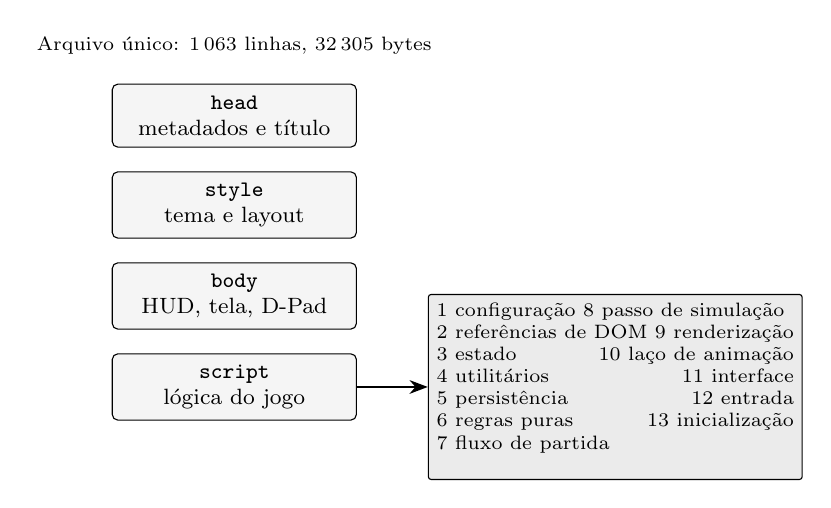
\begin{tikzpicture}[
			font=\footnotesize,
			bloco/.style={draw, rounded corners=2pt, align=center, fill=black!4, inner sep=4pt},
			interno/.style={draw, rounded corners=1pt, align=left, fill=black!8, font=\scriptsize, inner sep=3pt},
			>=Stealth,
			fl/.style={->, thick}
		]

		\node[bloco, minimum width=3.1cm, minimum height=0.8cm] (head) at (0,0) {\texttt{head}\\ metadados e título};
		\node[bloco, minimum width=3.1cm, minimum height=0.8cm, below=0.3cm of head] (style) {\texttt{style}\\ tema e layout};
		\node[bloco, minimum width=3.1cm, minimum height=0.8cm, below=0.3cm of style] (body) {\texttt{body}\\ HUD, tela, D-Pad};
		\node[bloco, minimum width=3.1cm, minimum height=0.8cm, below=0.3cm of body] (script) {\texttt{script}\\ lógica do jogo};

		\node[interno, right=0.9cm of script, anchor=west] (sec) {%
			1 configuração \hfill 8 passo de simulação\\
			2 referências de DOM \hfill 9 renderização\\
			3 estado \hfill 10 laço de animação\\
			4 utilitários \hfill 11 interface\\
			5 persistência \hfill 12 entrada\\
			6 regras puras \hfill 13 inicialização\\
			7 fluxo de partida \hfill \\
		};

		\draw[fl] (script) -- (sec);

		\node[font=\scriptsize, above=0.25cm of head] (tag) {Arquivo único: 1\,063 linhas, 32\,305 bytes};
	\end{tikzpicture}
	\legend{Fonte: elaborado pelo autor (2026) a partir de \texttt{index.html}. A restrição de artefato
	único (\texttt{CON-001}) impede a separação física entre módulos, de modo que o isolamento é obtido
	por funções de responsabilidade única dentro do mesmo arquivo.}
\end{figure}


A organização em seções numeradas é a resposta a \texttt{NFR-005} (código
comentado e organizado) e cumpre função operacional, não apenas estética: como o
processo de verificação precisa localizar trechos específicos por inspeção
textual, a previsibilidade da estrutura reduz o esforço de verificação.

A restrição \texttt{CON-001} (artefato único) tem uma consequência de projeto que
vale explicitar: sem módulos separados, não há como isolar a lógica de simulação
da lógica de apresentação por meio de fronteiras de arquivo. O isolamento foi
obtido por meio de funções com responsabilidade única dentro do mesmo arquivo, e
a separação é garantida por convenção, não por mecanismo. É um enfraquecimento
real da arquitetura em relação a uma solução modular --- aceito porque exigido
pela especificação.

\section{Máquina de estados da partida}
\label{sec:impl-fsm}

A partida é modelada como máquina de estados finitos com cinco estados:
\texttt{ready}, \texttt{running}, \texttt{paused}, \texttt{over} e \texttt{won}.
A Figura~\ref{fig:fsm} apresenta as transições.

%% ---------------------------------------------------------------------
%%  FIGURA - Maquina de estados da partida (DG-04)
%% ---------------------------------------------------------------------
\begin{figure}[htb]
	\caption{Máquina de estados da partida e transições}
	\label{fig:fsm}
	\centering
	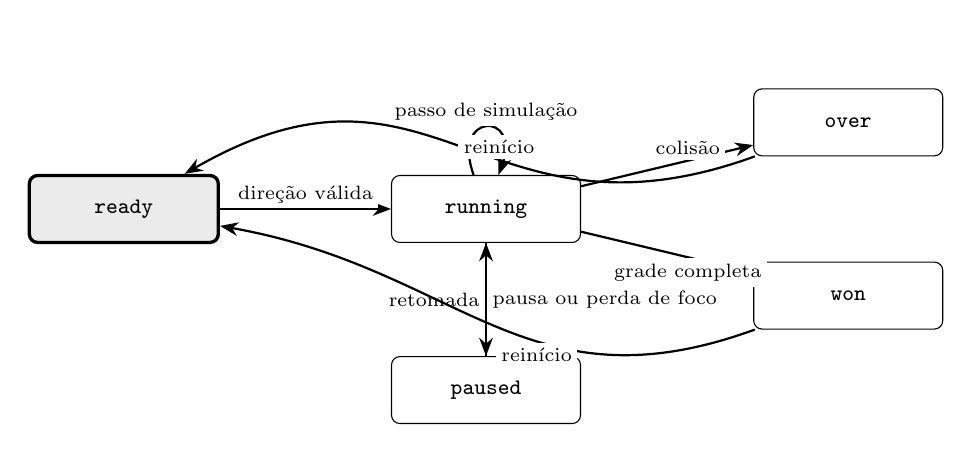
\begin{tikzpicture}[
			font=\footnotesize,
			estado/.style={draw, rounded corners=3pt, minimum width=2.4cm, minimum height=0.85cm, align=center},
			inicial/.style={estado, very thick, fill=black!8},
			>=Stealth,
			tr/.style={->, thick},
			rot/.style={font=\scriptsize, inner sep=2pt, fill=white}
		]

		\node[inicial] (ready) at (0,0) {\texttt{ready}};
		\node[estado] (run) at (4.6,0) {\texttt{running}};
		\node[estado] (pause) at (4.6,-2.3) {\texttt{paused}};
		\node[estado] (over) at (9.2,1.1) {\texttt{over}};
		\node[estado] (won) at (9.2,-1.1) {\texttt{won}};

		\draw[tr] (ready) -- node[rot, above] {direção válida} (run);
		\draw[tr] (run) -- node[rot, right] {pausa ou perda de foco} (pause);
		\draw[tr] (pause) -- node[rot, left] {retomada} (run);
		\draw[tr] (run) -- node[rot, pos=0.62, above] {colisão} (over);
		\draw[tr] (run) -- node[rot, pos=0.62, below] {grade completa} (won);

		\draw[tr] (run) to[out=110, in=70, looseness=7] node[rot, above] {passo de simulação} (run);

		\draw[tr] (over) to[out=200, in=30, looseness=1.3] node[rot, pos=0.42, above] {reinício} (ready);
		\draw[tr] (won) to[out=200, in=-10, looseness=1.15] node[rot, pos=0.4, below] {reinício} (ready);
	\end{tikzpicture}
	\legend{Fonte: elaborado pelo autor (2026) a partir de \texttt{index.html}, seção~7.
	O estado \texttt{won} não constava da solicitação original: ele foi criado para tratar o caso de
	borda ``grade completamente ocupada''.}
\end{figure}


Duas decisões de modelagem merecem registro. A primeira é a existência do estado
\texttt{won}, que não constava da solicitação original. Ele é necessário porque a
especificação declarou o caso de borda ``grade completamente ocupada''
(Seção~\ref{sec:esp-bordas}): sem esse estado, o sorteio do alvo retornaria um
valor inválido e o jogo entraria em estado inconsistente. A modelagem do caso de
borda forçou a criação de um estado. Esse é um exemplo concreto de como declarar
casos de borda altera o projeto, e não apenas os testes.

A segunda é que o estado \texttt{ready} não é apenas decorativo. Ele existe
porque a especificação exige que a movimentação comece somente após a primeira
entrada direcional válida (\texttt{FR-012}). A consequência é que a primeira
entrada precisa ser tratada de forma diferente das demais: como o jogador ainda
não se moveu, qualquer direção cardinal é aceita, inclusive a oposta à direção
inicial, e o corpo é reposicionado atrás da nova cabeça para evitar autocolisão
imediata. Sem esse tratamento, pressionar ``esquerda'' na tela inicial mataria o
jogador no primeiro passo.

\section{Laço de animação}
\label{sec:impl-loop}

O laço usa o mecanismo de requisição de quadro de animação
(\citeonline{mdn2024raf}), com acumulador de tempo para separar a simulação da
apresentação, conforme \texttt{FR-014}, \texttt{CON-004} e ADR-002. A
Figura~\ref{fig:game-loop} representa o fluxo.

%% ---------------------------------------------------------------------
%%  FIGURA - Laco de animacao com acumulador (DG-05)
%% ---------------------------------------------------------------------
\begin{figure}[htb]
	\caption{Laço de animação com acumulador de tempo e execução de passos}
	\label{fig:game-loop}
	\centering
	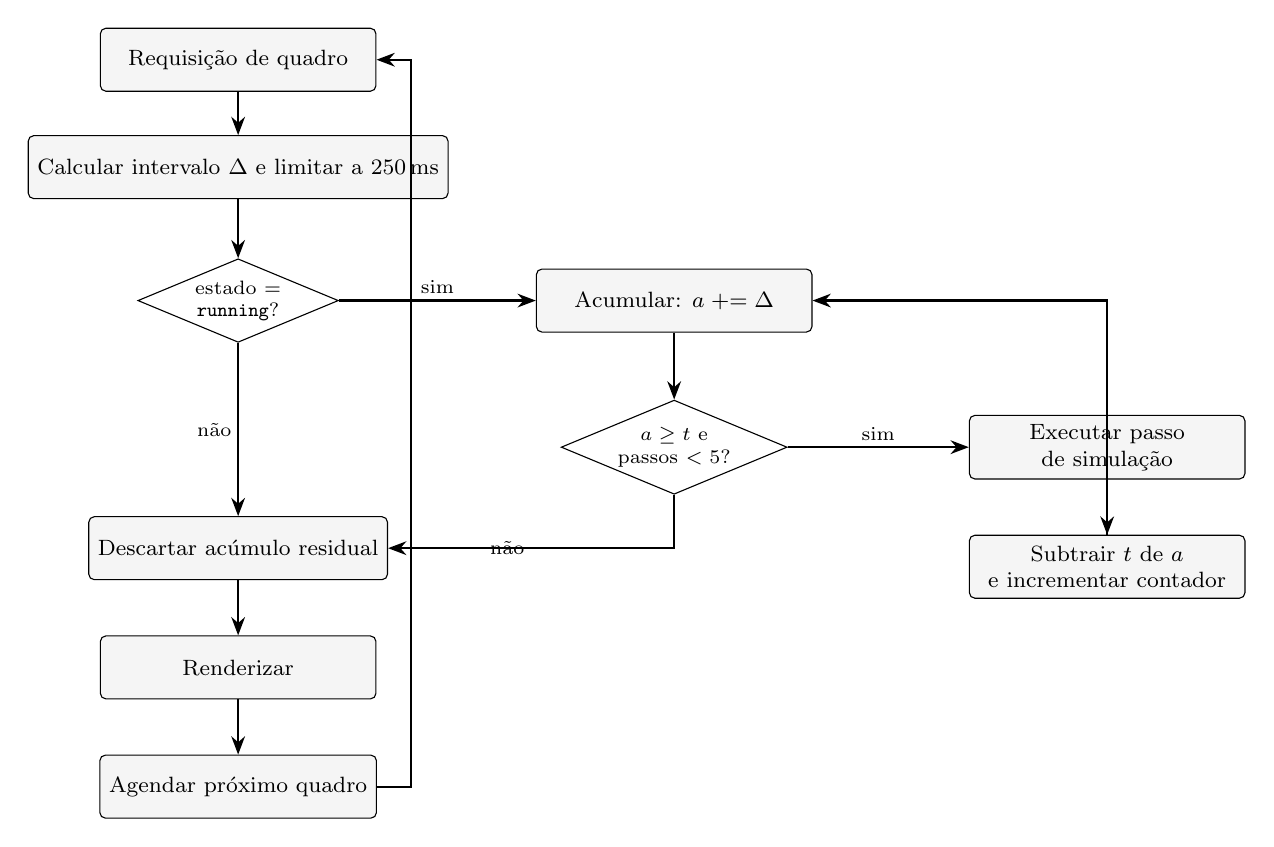
\begin{tikzpicture}[
			font=\footnotesize,
			passo/.style={draw, rounded corners=2pt, minimum width=3.5cm, minimum height=0.8cm, align=center, fill=black!4},
			dec/.style={draw, diamond, aspect=2.4, inner sep=1pt, align=center, font=\scriptsize},
			>=Stealth,
			fl/.style={->, thick},
			rot/.style={font=\scriptsize, inner sep=2pt}
		]

		\node[passo] (raf) at (0,0) {Requisição de quadro};
		\node[passo, below=0.55cm of raf] (delta) {Calcular intervalo $\Delta$ e limitar a 250\,ms};
		\node[dec, below=0.75cm of delta] (rodando) {estado =\\ \texttt{running}?};
		\node[passo, right=2.5cm of rodando] (acum) {Acumular: $a \mathrel{+}= \Delta$};
		\node[dec, below=0.85cm of acum] (suf) {$a \geq t$ e\\ passos $< 5$?};
		\node[passo, right=2.3cm of suf] (tick) {Executar passo\\ de simulação};
		\node[passo, below=0.7cm of tick] (dec2) {Subtrair $t$ de $a$\\ e incrementar contador};
		\node[passo, below=2.2cm of rodando] (desc) {Descartar acúmulo residual};
		\node[passo, below=0.7cm of desc] (render) {Renderizar};
		\node[passo, below=0.7cm of render] (loop) {Agendar próximo quadro};

		\draw[fl] (raf) -- (delta);
		\draw[fl] (delta) -- (rodando);
		\draw[fl] (rodando) -- node[rot, above] {sim} (acum);
		\draw[fl] (acum) -- (suf);
		\draw[fl] (suf) -- node[rot, above] {sim} (tick);
		\draw[fl] (tick) -- (dec2);
		\draw[fl] (dec2) |- (acum);
		\draw[fl] (suf) |- node[rot, pos=0.75, left] {não} (desc);
		\draw[fl] (rodando) -- node[rot, left] {não} (desc);
		\draw[fl] (desc) -- (render);
		\draw[fl] (render) -- (loop);
		\draw[fl] (loop) -- ++(2.2,0) |- (raf);
	\end{tikzpicture}
	\legend{Fonte: elaborado pelo autor (2026) a partir de \texttt{index.html}, seção~10.
	O teto de cinco passos por quadro e o descarte do acúmulo residual são as duas defesas contra a
	espiral da morte.}
\end{figure}


O trecho central está no Quadro~\ref{qua:codigo-loop}.

\begin{quadro}[htb]
	\caption{Trecho do laço de animação: acúmulo de tempo e execução de passos (excertado)}
	\label{qua:codigo-loop}
	\begin{lstlisting}[style=codigo]
const delta = Math.min(timestamp - state.lastTs, 250);
state.lastTs = timestamp;
state.elapsed += delta;

if (state.status === 'running') {
  state.acc += delta;
  let steps = 0;
  while (state.acc >= state.stepMs && steps < CONFIG.maxTicksPerFrame) {
    state.acc -= state.stepMs;
    steps += 1;
    tick();
    if (state.status !== 'running') { state.acc = 0; break; }
  }
  if (state.acc > state.stepMs * CONFIG.maxTicksPerFrame) state.acc = 0;
} else {
  state.acc = 0;
}
	\end{lstlisting}
	\legend{Fonte: \texttt{index.html}, seção~10.}
\end{quadro}

Três detalhes do trecho são decisões de engenharia, não acidentes de codificação.

\textbf{Limitação do passo de tempo.} A primeira linha limita o intervalo a
250\,ms. Sem esse limite, um retorno de segundo plano produziria um intervalo de
vários segundos e o jogador avançaria dezenas de células em um único quadro, sem
possibilidade de reação. O limite converte uma anomalia de temporização em uma
perda controlada de fluidez.

\textbf{Teto de passos por quadro.} A condição \texttt{steps < maxTicksPerFrame}
limita a quantidade de simulações executadas em um mesmo quadro. Sem esse teto, a
recuperação do atraso acumulado consumiria mais tempo de processamento do que o
atraso original, ampliando a defasagem --- fenômeno conhecido como espiral da
morte. O teto rompe o ciclo ao custo de a simulação ficar momentaneamente atrás
do tempo real.

\textbf{Descarte do acúmulo residual.} A linha final descarta o acúmulo quando
ele excede o teto multiplicado pelo intervalo. É a segunda linha de defesa contra
a mesma anomalia.

A Tabela~\ref{tab:tempos} registra as grandezas temporais do laço.

\begin{table}[htb]
	\caption{Grandezas temporais do laço de animação}
	\label{tab:tempos}
	\centering
	\footnotesize
	\begin{tabularx}{\textwidth}{@{}p{4.4cm} c X@{}}
		\toprule
		\textbf{Grandeza} & \textbf{Valor} & \textbf{Observação} \\
		\midrule
		Intervalo inicial entre passos & 140\,ms & Aproximadamente sete passos por segundo \\
		\addlinespace
		Intervalo mínimo & 68\,ms & Aproximadamente quinze passos por segundo \\
		\addlinespace
		Teto de passo de tempo & 250\,ms & Limite do intervalo aceito em um quadro \\
		\addlinespace
		Teto de passos por quadro & 5 & Proteção contra espiral da morte \\
		\addlinespace
		Taxa de quadro alvo & --- & Delegada ao navegador pelo mecanismo de requisição de quadro \\
		\bottomrule
	\end{tabularx}
	\legend{Fonte: elaborado pelo autor (2026) a partir de \texttt{index.html}.}
\end{table}

\section{Algoritmo de um passo de simulação}
\label{sec:impl-tick}

O passo de simulação é a unidade atômica do jogo. Sua ordem de operações é
determinada por ADR-004 e está representada na Figura~\ref{fig:tick}.

%% ---------------------------------------------------------------------
%%  FIGURA - Algoritmo de um passo de simulacao (DG-06)
%% ---------------------------------------------------------------------
\begin{figure}[htb]
	\caption{Algoritmo de um passo de simulação, com destaque para a ordem de ADR-004}
	\label{fig:tick}
	\centering
	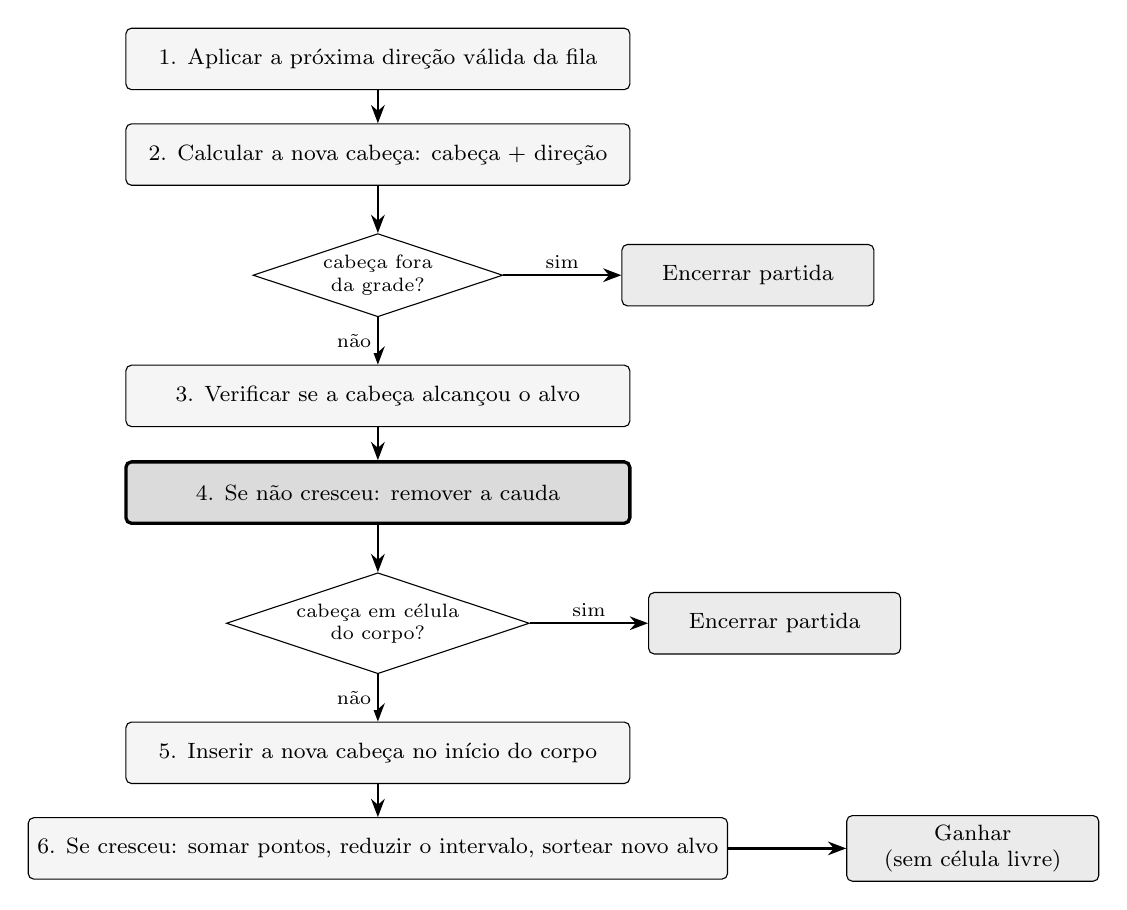
\begin{tikzpicture}[
			font=\footnotesize,
			acao/.style={draw, rounded corners=2pt, minimum width=6.4cm, minimum height=0.78cm, align=center, fill=black!4},
			critico/.style={acao, fill=black!14, very thick},
			saida/.style={draw, rounded corners=2pt, minimum width=3.2cm, minimum height=0.78cm, align=center, fill=black!8},
			dec/.style={draw, diamond, aspect=3.0, inner sep=1pt, align=center, font=\scriptsize},
			>=Stealth,
			fl/.style={->, thick},
			rot/.style={font=\scriptsize, inner sep=2pt, fill=white}
		]

		\node[acao] (a1) at (0,0) {1. Aplicar a próxima direção válida da fila};
		\node[acao, below=0.42cm of a1] (a2) {2. Calcular a nova cabeça: cabeça $+$ direção};
		\node[dec, below=0.6cm of a2] (d1) {cabeça fora\\ da grade?};
		\node[acao, below=0.6cm of d1] (a3) {3. Verificar se a cabeça alcançou o alvo};
		\node[critico, below=0.42cm of a3] (a4) {4. Se não cresceu: remover a cauda};
		\node[dec, below=0.6cm of a4] (d2) {cabeça em célula\\ do corpo?};
		\node[acao, below=0.6cm of d2] (a5) {5. Inserir a nova cabeça no início do corpo};
		\node[acao, below=0.42cm of a5] (a6) {6. Se cresceu: somar pontos, reduzir o intervalo, sortear novo alvo};

		\node[saida, right=1.5cm of d1] (o1) {Encerrar partida};
		\node[saida, right=1.5cm of d2] (o2) {Encerrar partida};
		\node[saida, right=1.5cm of a6, align=center] (o3) {Ganhar\\ (sem célula livre)};

		\draw[fl] (a1) -- (a2);
		\draw[fl] (a2) -- (d1);
		\draw[fl] (d1) -- node[rot, left] {não} (a3);
		\draw[fl] (d1) -- node[rot, above] {sim} (o1);
		\draw[fl] (a3) -- (a4);
		\draw[fl] (a4) -- (d2);
		\draw[fl] (d2) -- node[rot, left] {não} (a5);
		\draw[fl] (d2) -- node[rot, above] {sim} (o2);
		\draw[fl] (a5) -- (a6);
		\draw[fl] (a6) -- (o3);
	\end{tikzpicture}
	\legend{Fonte: elaborado pelo autor (2026) a partir de \texttt{index.html}, seção~8.
	O passo 4 é destacado porque sua posição \emph{antes} do teste de colisão (ADR-004) determina se
	ocupar a célula recém-liberada pela cauda é sobrevivência ou morte.}
\end{figure}


O Quadro~\ref{qua:codigo-tick} apresenta o trecho correspondente.

\begin{quadro}[htb]
	\caption{Trecho do passo de simulação: cálculo da cabeça, colisão e remoção da cauda (excertado)}
	\label{qua:codigo-tick}
	\begin{lstlisting}[style=codigo]
if (state.queue.length > 0) {
  state.dir = state.queue.shift();
}
const head = {
  x: state.snake[0].x + state.dir.x,
  y: state.snake[0].y + state.dir.y
};
if (head.x < 0 || head.y < 0 ||
    head.x >= CONFIG.cols || head.y >= CONFIG.rows) {
  endGame('collision');
  return;
}
const growing = state.food !== null && sameCell(head, state.food);
if (!growing) {
  state.snake.pop();
}
	\end{lstlisting}
	\legend{Fonte: \texttt{index.html}, seção~8.}
\end{quadro}

A ordem tem três propriedades que importam.

\textbf{A direção é aplicada antes do movimento.} A fila é consumida no início do
passo, de modo que a direção usada no cálculo corresponde exatamente à intenção
vigente naquele passo.

\textbf{A colisão de borda é testada antes de qualquer mutação do corpo.} Se a
cabeça saiu da grade, o estado não foi alterado. Isso mantém a consistência do
estado observável em caso de encerramento.

\textbf{A cauda é removida antes do teste de colisão com o corpo.} Essa é a
decisão ADR-004 e produz o comportamento declarado no caso de borda~5: mover para
a célula que a cauda acabou de liberar é sobrevivência, não morte. A ordem inversa
produziria a morte.

\section{Fila de entrada e bloqueio de inversão}
\label{sec:impl-entrada}

O bloqueio de inversão instantânea (\texttt{FR-005}) é implementado por fila de
capacidade limitada com validação contra a última direção de referência. A
Figura~\ref{fig:sequencia} apresenta a sequência de tratamento de uma entrada.

%% ---------------------------------------------------------------------
%%  FIGURA - Sequencia de tratamento de entrada (DG-08)
%% ---------------------------------------------------------------------
\begin{figure}[htb]
	\caption{Sequência de tratamento de uma entrada direcional}
	\label{fig:sequencia}
	\centering
	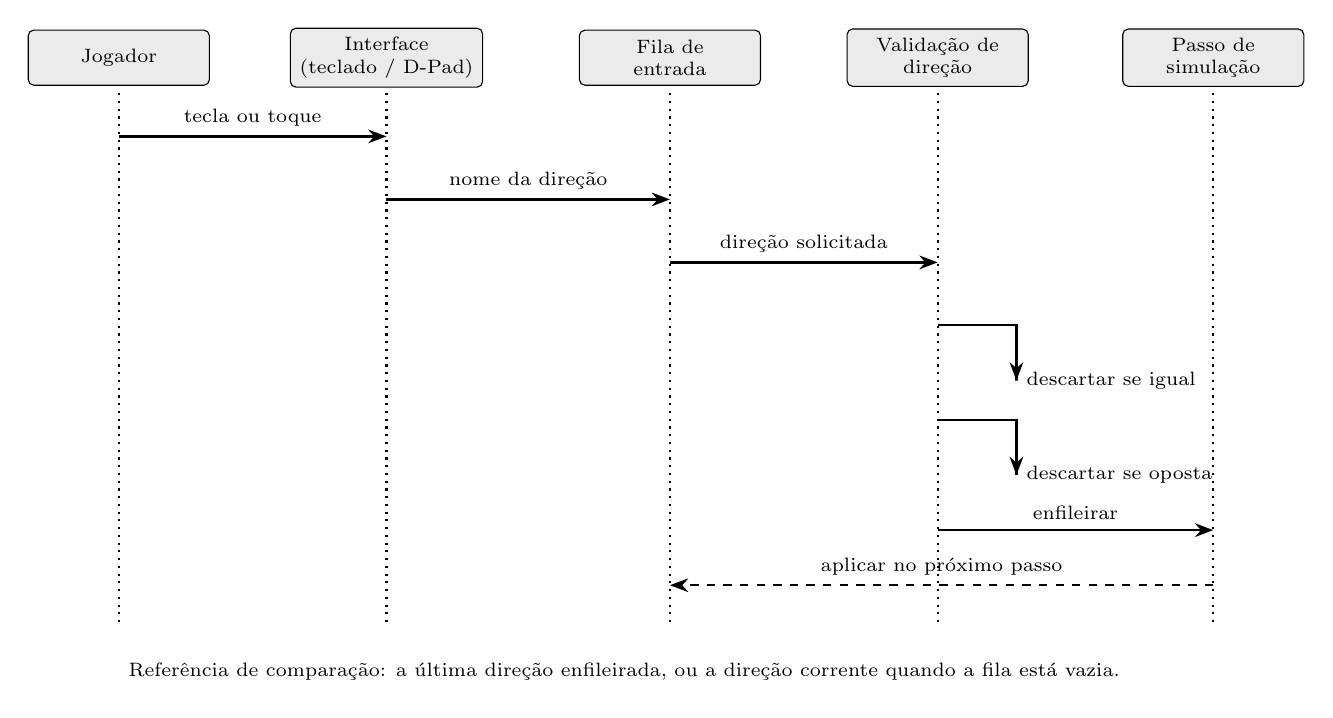
\begin{tikzpicture}[
			font=\scriptsize,
			ator/.style={draw, rounded corners=2pt, minimum width=2.3cm, minimum height=0.7cm, align=center, fill=black!8},
			>=Stealth,
			msg/.style={->, thick},
			ret/.style={->, thick, dashed}
		]

		% atores e linhas de vida
		\node[ator] (jog) at (0,0) {Jogador};
		\node[ator] (ui) at (3.4,0) {Interface\\ (teclado / D-Pad)};
		\node[ator] (fila) at (7.0,0) {Fila de\\ entrada};
		\node[ator] (val) at (10.4,0) {Validação de\\ direção};
		\node[ator] (pas) at (13.9,0) {Passo de\\ simulação};

		\foreach \x in {0,3.4,7.0,10.4,13.9} {
				\draw[dotted, thick] (\x,-0.45) -- (\x,-7.2);
			}

		\draw[msg] (0,-1.0) -- node[above, font=\scriptsize] {tecla ou toque} (3.4,-1.0);
		\draw[msg] (3.4,-1.8) -- node[above, font=\scriptsize] {nome da direção} (7.0,-1.8);
		\draw[msg] (7.0,-2.6) -- node[above, font=\scriptsize] {direção solicitada} (10.4,-2.6);

		\draw[msg] (10.4,-3.4) -- ++(1.0,0) -- ++(0,-0.7) -- node[right, font=\scriptsize, pos=0.55] {descartar se igual} (11.4,-4.1);
		\draw[msg] (10.4,-4.6) -- ++(1.0,0) -- ++(0,-0.7) -- node[right, font=\scriptsize, pos=0.55] {descartar se oposta} (11.4,-5.3);

		\draw[msg] (10.4,-6.0) -- node[above, font=\scriptsize] {enfileirar} (13.9,-6.0);
		\draw[ret] (13.9,-6.7) -- node[above, font=\scriptsize] {aplicar no próximo passo} (7.0,-6.7);

		\node[font=\scriptsize, align=left, anchor=west] at (0,-7.8)
		{Referência de comparação: a última direção enfileirada, ou a direção corrente quando a fila está vazia.};
	\end{tikzpicture}
	\legend{Fonte: elaborado pelo autor (2026) a partir de \texttt{index.html}, seção~6 (ADR-003).
	Comparar com a última direção \emph{enfileirada} permite duas mudanças de noventa graus no mesmo passo
	sem abrir a possibilidade de inversão de cento e oitenta graus.}
\end{figure}


O Quadro~\ref{qua:codigo-fila} apresenta o trecho.

\begin{quadro}[htb]
	\caption{Trecho do enfileiramento de direção com bloqueio de inversão (excertado)}
	\label{qua:codigo-fila}
	\begin{lstlisting}[style=codigo]
const reference = state.queue.length > 0
  ? state.queue[state.queue.length - 1]
  : state.dir;

if (sameCell(next, reference) || isOpposite(next, reference)) {
  return;
}
if (state.queue.length >= CONFIG.maxQueue) {
  state.queue.shift();
}
state.queue.push({ ...next });
	\end{lstlisting}
	\legend{Fonte: \texttt{index.html}, seção~6.}
\end{quadro}

A validação usa como referência a \emph{última direção enfileirada}, e não a
direção corrente, quando a fila não está vazia. A diferença é o que permite duas
mudanças de noventa graus em um mesmo passo curto --- por exemplo, direita seguida
de baixo --- sem permitir a inversão de cento e oitenta graus. Comparar apenas
com a direção corrente rejeitaria a segunda entrada, e o jogador perderia o
comando; comparar com a fila preserva a intenção sem abrir a possibilidade de
inversão.

\section{Sorteio do alvo}
\label{sec:impl-alvo}

O sorteio do alvo (\texttt{FR-006}) impede que o alvo apareça sobre o corpo. A
estratégia tem duas fases. Na primeira, sorteia-se uma célula aleatória e verifica-se
sua presença em um conjunto de ocupação, por até 500 tentativas. Se todas
falharem, executa-se uma varredura determinística em ordem de linha e coluna,
retornando a primeira célula livre.

A escolha de duas fases é uma decisão de robustez. A amostragem aleatória é
adequada enquanto a ocupação é baixa; quando o tabuleiro fica quase cheio, a
probabilidade de acerto cai e o custo esperado de tentativas cresce. A varredura
determinística garante término e, se nenhuma célula estiver livre, retorna valor
nulo, que o passo de simulação interpreta como vitória --- o estado
\texttt{won}.

O Quadro~\ref{qua:codigo-alvo} apresenta o núcleo do sorteio.

\begin{quadro}[htb]
	\caption{Trecho do sorteio de célula livre para o alvo (excertado)}
	\label{qua:codigo-alvo}
	\begin{lstlisting}[style=codigo]
const occupied = new Set(state.snake.map(function (cell) {
  return cell.x + ',' + cell.y;
}));

for (let attempt = 0; attempt < CONFIG.maxFoodAttempts; attempt += 1) {
  const cell = { x: randomInt(CONFIG.cols), y: randomInt(CONFIG.rows) };
  if (!occupied.has(cell.x + ',' + cell.y)) {
    return cell;
  }
}
	\end{lstlisting}
	\legend{Fonte: \texttt{index.html}, seção~6.}
\end{quadro}

Uma nota de eficiência: a codificação da célula como texto para uso em conjunto
tem custo de alocação. A alternativa sem alocação seria uma matriz de ocupação
reutilizada entre passos, o que exigiria limpeza seletiva a cada passo e
introduziria risco de estado residual. A escolha pela legibilidade e
previsibilidade, com o custo de alocação assumido, é coerente com
\texttt{NFR-005} e com o tamanho da grade (24 por 24 células).

\section{Persistência do recorde}
\label{sec:impl-persistencia}

A persistência (\texttt{FR-010}) está isolada em duas funções envoltas em
tratamento de exceção, conforme ADR-006. A gravação ocorre no momento em que a
pontuação supera o recorde, e não apenas no encerramento da partida.

A escolha de gravar durante a partida tem uma consequência favorável: se a página
for fechada abruptamente, o recorde conquistado não se perde. O custo é uma
escrita no armazenamento por item consumido, custo irrelevante na escala do jogo.
A leitura ocorre uma única vez, na inicialização.

O tratamento de exceção cobre dois cenários reais: navegação privada com
armazenamento restrito e política de armazenamento desabilitada pelo usuário. Em
ambos, a função de leitura retorna zero e o jogo permanece jogável com o recorde
válido apenas na sessão corrente. A falha é degradada, não propagada.

\section{Renderização}
\label{sec:impl-render}

A renderização ocorre em superfície vetorial bidimensional
(\citeonline{mdn2024canvas}) e segue ADR-001. Três decisões a caracterizam.

\textbf{Ajuste à densidade da tela.} O Quadro~\ref{qua:codigo-resize} mostra o
ajuste, que atende \texttt{NFR-006}. A razão de pixels é limitada a~2 para evitar
custo de desenho desnecessário em telas de densidade muito alta, nas quais o
ganho visual seria imperceptível e o custo de memória, não.

\begin{quadro}[htb]
	\caption{Trecho do ajuste da superfície de desenho à densidade da tela (excertado)}
	\label{qua:codigo-resize}
	\begin{lstlisting}[style=codigo]
const rect = dom.canvas.getBoundingClientRect();
const cssSize = Math.max(1, Math.round(rect.width));
const dpr = Math.min(window.devicePixelRatio || 1, 2);

dom.canvas.width = Math.round(cssSize * dpr);
dom.canvas.height = Math.round(cssSize * dpr);
ctx.setTransform(dpr, 0, 0, dpr, 0, 0);

view.size = cssSize;
view.cell = cssSize / CONFIG.cols;
	\end{lstlisting}
	\legend{Fonte: \texttt{index.html}, seção~9.}
\end{quadro}

\textbf{Conversão de célula para pixel em um único ponto.} O tamanho da célula é
calculado uma única vez, e todo o desenho deriva dele. Não há coordenada de pixel
literal no código de desenho, exceto as relativas à própria célula (espessura de
borda, deslocamento dos olhos). Essa disciplina é o que permite alterar o número
de colunas da grade sem tocar no código de desenho.

\textbf{Observação de redimensionamento.} O ajuste é reexecutado quando o
contêiner muda de tamanho, por observador de redimensionamento quando disponível
e por evento de janela como alternativa. Isso cobre rotação de tela e
redimensionamento de janela sem recarregar a página.

A Figura~\ref{fig:interface} registra visualmente o resultado da implementação no
estado de fim de jogo: o tema escuro com acentos neon (\texttt{NFR-003}), o
layout centralizado e responsivo (\texttt{NFR-002}), o placar com as duas
grandezas (\texttt{FR-009} e \texttt{FR-010}), a sobreposição de fim de jogo com
o botão de reinício (\texttt{FR-011}) e os quatro controles direcionais
(\texttt{FR-004}).

Cabe uma advertência sobre o estatuto dessa imagem. Ela é \emph{registro visual},
não verificação. Nenhum critério de aceitação é satisfeito ou reprovado com base
em uma captura de tela: os requisitos que ela ilustra são verificados por
observação de comportamento (Tabela~\ref{tab:ca-resultados}) ou, quando não
possuem critério, permanecem sem verificação. Ilustrar um requisito em uma figura
não o promove a verificado.

%% ---------------------------------------------------------------------
%%  FIGURA - Registro visual da interface implementada
%%
%%  A imagem NAO esta em figures/: ela e a captura de tela real do produto,
%%  mantida em images/ na raiz do repositorio (ver \graphicspath em main.tex).
%%  O caminho e resolvido por ../images/screenshot_gaming.png.
%% ---------------------------------------------------------------------
\begin{figure}[htb]
	\caption{Interface implementada, no estado de fim de jogo com placar preenchido}
	\label{fig:interface}
	\centering
	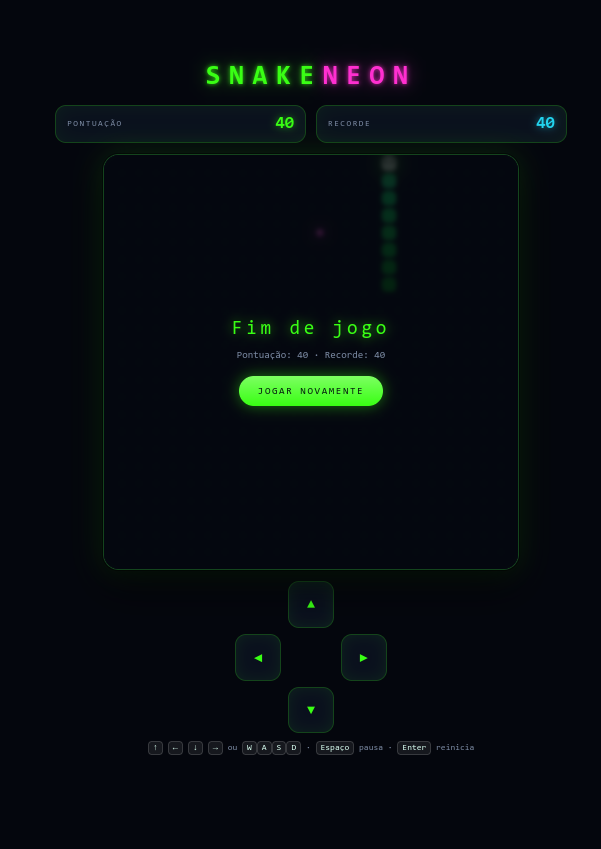
\includegraphics[width=0.74\textwidth]{screenshot_gaming.png}
	\legend{Fonte: arquivo \texttt{images/screenshot\_gaming.png}. Captura de tela do sistema-alvo
	em execução, no estado \texttt{over}. São visíveis: o título da aplicação; o placar com
	pontuação atual e melhor pontuação, ambas em 40; o tabuleiro com o corpo do jogador; a
	sobreposição de fim de jogo com a pontuação final e o botão de reinício; os quatro botões
	direcionais; e a linha de atalhos de teclado. Esta figura é \emph{registro visual} da
	interface, não verificação de critério de aceitação --- a verificação está no
	Capítulo~\ref{cap:resultados}.}
\end{figure}


\section{Acessibilidade e resposta a preferências}
\label{sec:impl-acessibilidade}

Três medidas atendem \texttt{NFR-009} e às diretrizes de acessibilidade para
conteúdo web (\citeonline{w3c2023wcag22}).

\textbf{Preferência de movimento reduzido.} A animação pulsante do alvo é
desativada e as transições de interface são reduzidas quando o sistema operacional
declara essa preferência. A escolha é relevante porque a pulsação é o único
elemento puramente decorativo com movimento contínuo no produto.

\textbf{Foco visível.} Os elementos interativos têm indicação de foco explícita,
o que permite operá-los por teclado. Sem isso, os botões direcionais seriam
inacessíveis a quem não usa apontador.

\textbf{Região viva para leitores de tela.} Mudanças de estado da partida são
anunciadas em região com semântica de estado, de modo que a transição para pausa
ou para fim de jogo não seja silenciosa para tecnologias assistivas.

Registra-se uma limitação: os controles direcionais são botões com rótulo
textual, o que os torna acessíveis, mas a superfície de desenho do jogo não
oferece descrição textual do estado corrente para leitores de tela. Um jogo
acessível a pessoas cegas exigiria uma representação textual do tabuleiro, que
não foi especificada e está fora do escopo deste trabalho.

\section{Verificação de restrições durante a implementação}
\label{sec:impl-restricoes}

A Tabela~\ref{tab:restricoes-verificacao} registra como cada restrição foi
verificada na implementação.

\begin{table}[htb]
	\caption{Verificação das restrições na implementação}
	\label{tab:restricoes-verificacao}
	\centering
	\footnotesize
	\begin{tabularx}{\textwidth}{@{}p{1.7cm} X p{2.6cm}@{}}
		\toprule
		\textbf{ID} & \textbf{Restrição} & \textbf{Verificação} \\
		\midrule
		CON-001 & Artefato único & Inspeção: um único arquivo, um bloco de estilo, um bloco de script \\
		\addlinespace
		CON-002 & Apenas CSS e JavaScript nativos & Inspeção: ausência de referências de rede e de dependências \\
		\addlinespace
		CON-003 & Configuração centralizada & Inspeção: objeto de configuração único, congelado, com sete campos \\
		\addlinespace
		CON-004 & Sem temporizador fixo para simulação & Inspeção: laço por requisição de quadro com acumulador \\
		\bottomrule
	\end{tabularx}
	\legend{Fonte: elaborado pelo autor (2026). A especificação do alvo declara quatro restrições
	(\texttt{CON-001} a \texttt{CON-004}); as restrições de hardware do material de origem do
	framework não têm correspondência no produto (ver P-26).}
\end{table}

\section{Síntese do capítulo}
\label{sec:impl-sintese}

A implementação materializou as sete decisões arquiteturais em 1\,063 linhas
organizadas em treze seções. Os pontos de maior consequência para o
comportamento observável são a ordem entre remoção da cauda e teste de colisão
(ADR-004), a referência usada na validação da fila de entrada (ADR-003) e o
tratamento do estado inicial (FR-012). O Capítulo~\ref{cap:resultados} verifica
se o comportamento resultante corresponde ao especificado.

%% =====================================================================
%%  CAPITULO 8 - EXPERIMENTOS E RESULTADOS
%% =====================================================================

\chapter{Experimentos e Resultados}
\label{cap:resultados}

Este capítulo reporta o protocolo de verificação e os resultados obtidos.
Reportam-se apenas resultados efetivamente observados; o que não foi verificado
está enumerado na Seção~\ref{sec:res-nao-verificado}.

\section{Protocolo de verificação}
\label{sec:res-protocolo}

A verificação executou os doze critérios de aceitação do Quadro~\ref{qua:ca},
mais uma medição quantitativa do intervalo entre passos de simulação. Para cada
critério, o resultado foi classificado como satisfeito, não satisfeito ou não
verificável. A classificação não admitiu valor intermediário.

Dois procedimentos foram usados. A inspeção estática verificou propriedades
estruturais que não dependem de execução, por busca textual no artefato. A
execução observada verificou comportamento, por automação de navegador com envio
de eventos e leitura do estado observável da página, incluindo amostragem de
pixels da superfície de desenho.

A opção por observação externa, sem instrumentar o produto, é deliberada. Um
teste que exige alterar o código para expor o estado interno mede o código
alterado, não o código entregue. A leitura de pixels contorna essa objeção: ela
observa exatamente o que o usuário vê.

\section{Resultados por critério de aceitação}
\label{sec:res-ca}

A Tabela~\ref{tab:ca-resultados} consolida os resultados. Cada linha registra o
critério, o instrumento usado, a observação e o resultado.

\begin{table}[htb]
	\caption{Resultado da verificação por critério de aceitação}
	\label{tab:ca-resultados}
	\centering
	\scriptsize
	\begin{tabularx}{\textwidth}{@{}p{1.3cm} p{2.1cm} X c@{}}
		\toprule
		\textbf{CA} & \textbf{Instrumento} & \textbf{Observação registrada} & \textbf{Resultado} \\
		\midrule
		CA-001 & Inspeção estática & Busca por referências de rede, de script e de estilo retornou vazio; exatamente um bloco de estilo e um de script & Satisfeito \\
		\addlinespace
		CA-002 & Execução observada & Entrada ``direita'' seguida de ``esquerda'': o jogador manteve o sentido e encerrou por colisão com a borda direita & Satisfeito \\
		\addlinespace
		CA-003 & Execução observada & Agente de teste orientado por busca em largura: pontuação passou de 0 para 10 após consumo & Satisfeito \\
		\addlinespace
		CA-004 & Execução observada & 25 amostras da célula do alvo; nenhuma sobreposição com células de corpo & Satisfeito \\
		\addlinespace
		CA-005 & Execução observada & Colisão com a borda: título da sobreposição passou a ``Fim de jogo'' e botão de reinício exibido & Satisfeito \\
		\addlinespace
		CA-006 & Execução observada & Após crescimento, giro fechado em quatro células encerrou a partida com a cabeça em célula interior (6,6), longe das bordas & Satisfeito \\
		\addlinespace
		CA-007 & Execução observada & Chave de armazenamento local com valor ``10'' e, em execução posterior, ``100''; valor mantido após recarregar & Satisfeito \\
		\addlinespace
		CA-008 & Execução observada & Acionamento do botão superior moveu a cabeça de (11,11) para (12,9) & Satisfeito \\
		\addlinespace
		CA-009 & Execução observada & Sobreposição visível antes; oculta após a primeira direção válida & Satisfeito \\
		\addlinespace
		CA-010 & Execução observada & Estado ``Pausado'': cabeça imóvel em (12,9) por 600\,ms; retomada ocultou a sobreposição & Satisfeito \\
		\addlinespace
		CA-011 & Execução observada & Registro de erros e exceções do console vazio ao longo de todas as execuções & Satisfeito \\
		\addlinespace
		CA-012 & Medição & Intervalo médio 133\,ms com pontuação abaixo de 40 e 105\,ms com pontuação igual ou superior a 80 (Seção~\ref{sec:res-velocidade}) & Satisfeito \\
		\bottomrule
	\end{tabularx}
	\legend{Fonte: elaborado pelo autor (2026) a partir de \texttt{docs/05-testing/snake-game-evidence.md}.}
\end{table}

Substituindo na Equação~(\ref{eq:cobertura}), obtém-se

\begin{equation}
	A = \frac{12}{12} = 1{,}00,
	\label{eq:resultado-cobertura}
\end{equation}

\noindent isto é, todos os critérios de aceitação declarados foram satisfeitos.
O alcance dessa afirmação está limitado ao que está escrito na
Seção~\ref{sec:res-nao-verificado}.

\section{Cobertura de rastreabilidade}
\label{sec:res-rastreabilidade}

Além do resultado por critério, mediu-se a cobertura de rastreabilidade: a fração
de requisitos que possui critério de aceitação associado. A
Tabela~\ref{tab:cobertura-req} apresenta o resultado, obtido por contagem direta
na especificação.

\begin{table}[htb]
	\caption{Cobertura de rastreabilidade por classe de requisito}
	\label{tab:cobertura-req}
	\centering
	\footnotesize
	\begin{tabularx}{\textwidth}{@{}p{3.4cm} c c c c@{}}
		\toprule
		\textbf{Classe} & \textbf{Total} & \textbf{Com CA} & \textbf{Parcial} & \textbf{Cobertura} \\
		\midrule
		Requisitos funcionais & 15 & 11 & 1 & 73,3\,\% \\
		\addlinespace
		Requisitos não funcionais & 9 & 2 & 0 & 22,2\,\% \\
		\addlinespace
		\textbf{Total} & \textbf{24} & \textbf{13} & \textbf{1} & \textbf{54,2\,\%} \\
		\bottomrule
	\end{tabularx}
	\legend{Fonte: elaborado pelo autor (2026), por contagem em \texttt{spec.md}.
	``Parcial'' indica requisito coberto apenas em parte pelo critério associado.}
\end{table}

Os requisitos funcionais sem critério dedicado são \texttt{FR-002} (uso da
superfície de desenho), \texttt{FR-009} (exibição do placar) e \texttt{FR-014}
(laço de animação). \texttt{FR-011} está parcialmente coberto: o critério
\texttt{CA-005} verifica a exibição da tela de fim de jogo, mas não o
funcionamento do botão de reinício, que foi observado empiricamente sem
critério correspondente.

A assimetria entre as duas classes é o achado mais informativo desta seção. A
cobertura de requisitos funcionais é de 73,3\,\%, enquanto a de requisitos não
funcionais é de 22,2\,\%. A diferença não é acidental: requisitos funcionais
descrevem comportamento observável e convertem-se naturalmente em teste;
requisitos não funcionais, quando enunciados como atributos, não geram teste
óbvio --- e, sem teste, não geram critério. A consequência é que sete dos nove
requisitos não funcionais ficaram fora de qualquer portão de aceitação.

Esse resultado não decorre do framework, e sim da especificação que o framework
aceitou como válida. O portão G1 exige que existam requisito \emph{e} critério
antes da implementação; ele não exige que \emph{todo} requisito tenha critério.
Essa é uma lacuna do portão, identificada por autocrítica e discutida na
Seção~\ref{sec:disc-lacunas-do-gate}.

\section{Verificação de propriedades estruturais}
\label{sec:res-estruturais}

A inspeção estática produziu as seguintes observações concretas:

\begin{itemize}
	\item um único arquivo, com exatamente um bloco de estilo e um bloco de script;
	\item nenhuma referência de rede a script, estilo, fonte ou imagem em qualquer ponto do artefato;
	\item sete campos no objeto de configuração, com valores idênticos aos especificados na Tabela~\ref{tab:constantes};
	\item ausência de temporizador de intervalo fixo para a simulação, conforme \texttt{CON-004};
	\item treze seções comentadas, conforme \texttt{NFR-005}.
\end{itemize}

Essas observações sustentam \texttt{CA-001} e as restrições \texttt{CON-001} a
\texttt{CON-004}. Elas são o tipo de evidência mais barato de produzir e o mais
barato de reproduzir, porque não depende de ambiente de execução.

\section{Medição do intervalo entre passos}
\label{sec:res-velocidade}

A única medição quantitativa de comportamento contínuo foi o intervalo entre
passos de simulação, previsto pela Equação~(\ref{eq:velocidade-simplificada}) e
exigido por \texttt{FR-015} e \texttt{CA-012}.

\subsection{Procedimento}
\label{subsec:res-procedimento}

Um agente de teste jogou a partida de forma autônoma, localizando o alvo e a
cabeça por amostragem de pixels e escolhendo o caminho mais curto por busca em
largura sobre a grade livre. A cada mudança de posição da cabeça, registrou-se um
par (instante, pontuação corrente). A partida foi conduzida até a pontuação de
100 pontos, sem encerramento por colisão.

Foram amostrados 184 movimentos. Os intervalos foram agrupados em duas faixas de
pontuação e a média foi calculada pela Equação~(\ref{eq:intervalo-medio}).

\subsection{Resultado}
\label{subsec:res-resultado-velocidade}

A Tabela~\ref{tab:velocidade} confronta o valor medido com o intervalo previsto
pelo modelo da Equação~(\ref{eq:velocidade-simplificada}) para a faixa
correspondente.

\begin{table}[htb]
	\caption{Intervalo médio entre passos medido e previsto, por faixa de pontuação}
	\label{tab:velocidade}
	\centering
	\footnotesize
	\begin{tabularx}{\textwidth}{@{}p{3.2cm} c c c c@{}}
		\toprule
		\textbf{Faixa de pontuação} & \textbf{Média medida} & \textbf{Previsto (mín.)} & \textbf{Previsto (máx.)} & \textbf{Coerente} \\
		\midrule
		Abaixo de 40 pontos & 133\,ms & 128\,ms & 140\,ms & Sim \\
		\addlinespace
		80 pontos ou mais & 105\,ms & 100\,ms & 108\,ms & Sim \\
		\bottomrule
	\end{tabularx}
	\legend{Fonte: elaborado pelo autor (2026). Previsto pela Equação~(\ref{eq:velocidade-simplificada})
	nos extremos de cada faixa. Número de amostras por faixa não retido no registro de evidência --- ver P-11.}
\end{table}

Os dois valores medidos caem dentro do intervalo previsto para a faixa
correspondente, com desvio de 1\,ms em relação ao ponto médio de cada intervalo
previsto. A diferença entre as duas faixas é de 28\,ms, contra 28\,ms previstos
na comparação dos pontos médios (134\,ms e 104\,ms). A direção da variação ---
intervalo menor com pontuação maior --- coincide com a exigida por
\texttt{FR-015}.

Três advertências sobre a interpretação acompanham esse resultado.

\textbf{A medição é um limite superior.} O ciclo de observação introduz atraso
positivo: o instante registrado é posterior ao instante real da mudança de
posição. Os valores medidos não devem ser lidos como estimativas do parâmetro
\texttt{stepMs}, e sim como valores comparáveis entre si.

\textbf{A média de faixa pressupõe distribuição aproximadamente uniforme da
pontuação dentro da faixa.} Essa suposição não foi verificada. Ela é plausível
para a faixa alta, que cobre dois itens consumidos, mas não foi controlada.

\textbf{A amostra é única.} Não houve repetição do experimento, e portanto não há
intervalo de confiança nem teste de hipótese. A conclusão sustentada é de
coerência entre o medido e o previsto, não de significância estatística.

A Figura~\ref{fig:velocidade} representa a curva prevista pela especificação e
posiciona os dois valores medidos. A curva é \emph{modelo}, não medição; os dois
pontos são \emph{medição}, não modelo. A distinção é mantida visualmente e na
legenda.

%% ---------------------------------------------------------------------
%%  FIGURA - Curva do modelo de velocidade e pontos medidos (DG-11)
%%
%%  ATENCAO METODOLOGICA: a curva e o MODELO definido na especificacao
%%  (Equacao da secao 6.8). Os dois pontos sao MEDICOES da secao 8.5.
%%  Modelo e medicao nunca sao misturados nesta figura.
%% ---------------------------------------------------------------------
\begin{figure}[htb]
	\caption{Curva do modelo de velocidade da especificação e os dois valores medidos}
	\label{fig:velocidade}
	\centering
	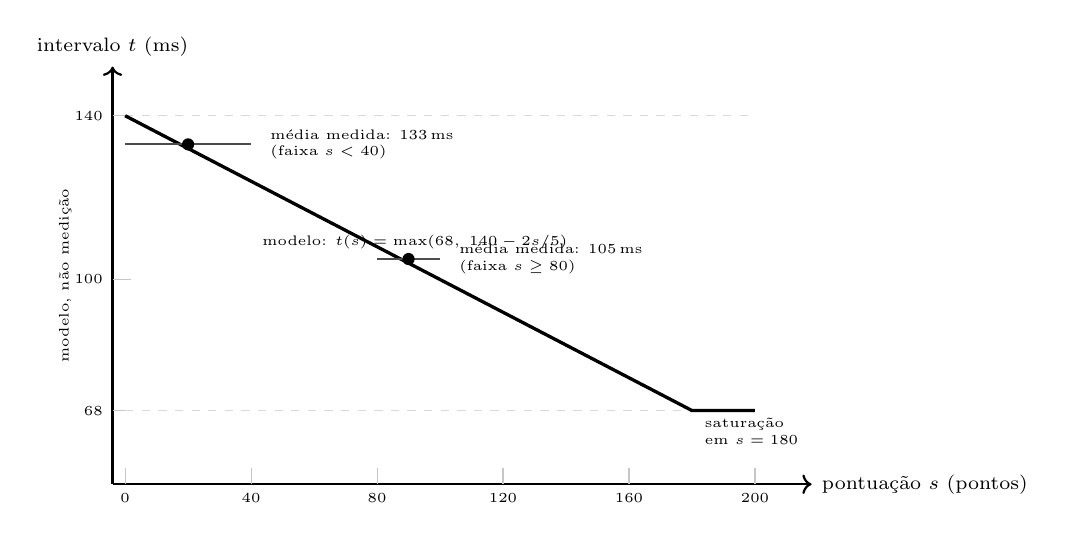
\begin{tikzpicture}[
			font=\scriptsize,
			x=0.040cm,
			y=0.052cm
		]

		% ---- eixos -----------------------------------------------------
		\draw[->, thick] (-4,50) -- (218,50) node[right] {pontuação $s$ (pontos)};
		\draw[->, thick] (-4,50) -- (-4,152) node[above, align=center] {intervalo $t$ (ms)};

		% ---- grade e marcas -------------------------------------------
		\foreach \x in {0,40,80,120,160,200} {
				\draw[gray!45, thin] (\x,50) -- (\x,54);
				\node[below, font=\tiny] at (\x,50) {\x};
			}
		\foreach \y in {68,100,140} {
				\draw[gray!45, thin] (-4,\y) -- (2,\y);
				\node[left, font=\tiny] at (-4,\y) {\y};
			}
		\draw[gray!30, dashed, thin] (0,68) -- (200,68);
		\draw[gray!30, dashed, thin] (0,140) -- (200,140);

		% ---- curva do modelo t(s) = max(68, 140 - 2s/5) ---------------
		\draw[very thick] (0,140) -- (180,68) -- (200,68);
		\node[above, font=\tiny, align=center] at (92,105) {modelo: $t(s) = \max(68,\; 140 - 2s/5)$};
		\node[right, font=\tiny, align=left] at (181,63) {saturação\\ em $s = 180$};

		% ---- faixas medidas ------------------------------------------
		% faixa baixa: pontuacao < 40, media medida 133 ms
		\draw[thick, black!70] (0,133) -- (40,133);
		\fill[black] (20,133) circle (2.2pt);
		\node[right, font=\tiny, align=left] at (43,133) {média medida: 133\,ms\\(faixa $s < 40$)};

		% faixa alta: pontuacao >= 80, media medida 105 ms
		\draw[thick, black!70] (80,105) -- (100,105);
		\fill[black] (90,105) circle (2.2pt);
		\node[right, font=\tiny, align=left] at (103,105) {média medida: 105\,ms\\(faixa $s \geq 80$)};

		% ---- anotacao do eixo y --------------------------------------
		\node[rotate=90, anchor=south, font=\tiny] at (-14,101) {modelo, não medição};
	\end{tikzpicture}
	\legend{Fonte: elaborado pelo autor (2026). A \textbf{curva} é o modelo declarado na especificação
	(Equação~(\ref{eq:velocidade-simplificada})), não uma medição. As \textbf{barras horizontais} são as
	faixas de pontuação sobre as quais cada média foi calculada, e os \textbf{círculos} são as médias
	medidas na Seção~\ref{sec:res-velocidade}. Os valores medidos incluem atraso positivo do ciclo de
	observação e não devem ser lidos como estimativas do parâmetro \texttt{stepMs}.}
\end{figure}


\section{Comportamentos observados sem critério correspondente}
\label{sec:res-extras}

Durante a verificação, quatro comportamentos foram observados mas não possuem
critério de aceitação associado. Registrá-los é obrigatório do ponto de vista da
integridade: são resultados, ainda que não estivessem previstos como testes.

\begin{enumerate}
	\item O reinício por tecla de confirmação na tela de fim de jogo restaura o estado e inicia a movimentação.
	\item O reinício por tecla R restaura a partida a partir de qualquer estado ativo.
	\item A perda de foco da janela provoca pausa automática.
	\item Girando em quadrado com comprimento quatro, o jogador sobrevive; a partir de comprimento cinco, colide consigo mesmo. Esse comportamento é a consequência observável de ADR-004 e confirma materialmente o caso de borda~5.
\end{enumerate}

O item 4 é o de maior valor para o trabalho, porque converte uma decisão
arquitetural em comportamento observável e, portanto, em evidência. Ele mostra
que ADR-004 não é uma preferência de estilo: produz diferença verificável no
comportamento do produto para a mesma especificação de requisitos.

\section{O que não foi verificado}
\label{sec:res-nao-verificado}

A Tabela~\ref{tab:nao-verificado} enumera o que ficou fora da verificação. Nenhum
item foi preenchido por estimativa.

\begin{table}[htb]
	\caption{Itens não verificados e razão}
	\label{tab:nao-verificado}
	\centering
	\footnotesize
	\begin{tabularx}{\textwidth}{@{}p{4.6cm} X@{}}
		\toprule
		\textbf{Item} & \textbf{Razão} \\
		\midrule
		Controles de toque em dispositivo móvel físico & Verificado apenas por emulação de evento de apontador em navegador de desktop. A diretriz do framework estabelece que emulação não promove o nível de evidência. Pendência registrada no projeto como T-016. \\
		\addlinespace
		Consumo de memória e taxa de quadros & Não instrumentado. Nenhuma meta foi declarada na especificação, e portanto nenhum critério existe. \\
		\addlinespace
		Responsividade em todas as larguras de 320\,px a 1920\,px & Verificada por cálculo de caixa de layout em uma largura e por inspeção dos pontos de quebra; não amostrada em todas as larguras. \\
		\addlinespace
		Leitores de tela e tecnologias assistivas & A estrutura semântica foi inspecionada; não houve teste com leitor de tela real. \\
		\addlinespace
		Navegadores alternativos ao motor Chromium & Não testado. A especificação não declara matriz de compatibilidade. \\
		\addlinespace
		Comportamento sob armazenamento local indisponível & O tratamento de exceção existe por inspeção, mas o cenário não foi reproduzido em execução. \\
		\bottomrule
	\end{tabularx}
	\legend{Fonte: elaborado pelo autor (2026).}
\end{table}

\section{Síntese do capítulo}
\label{sec:res-sintese}

A verificação produziu três resultados: doze de doze critérios de aceitação
satisfeitos, uma cobertura de rastreabilidade de 54,2\,\% sobre o conjunto de
requisitos, com forte assimetria entre requisitos funcionais (73,3\,\%) e não
funcionais (22,2\,\%), e uma medição de intervalo entre passos coerente com o
modelo da especificação em duas faixas de pontuação, com diferença de 28\,ms entre
elas. Seis itens permaneceram fora da verificação, e nenhum foi preenchido por
estimativa.

%% =====================================================================
%%  CAPITULO 9 - DISCUSSAO
%% =====================================================================

\chapter{Discussão}
\label{cap:discussao}

Este capítulo interpreta os resultados, confronta-os com o problema e a
hipótese, identifica as lacunas que a própria verificação revelou e retoma as
ameaças à validade. A seção final discute em que medida os achados são
generalizáveis.

\section{Retomada do problema e da hipótese}
\label{sec:disc-problema}

O problema enunciado na Seção~\ref{sec:problema} tinha três componentes:
rastreabilidade a requisito, verificabilidade por critério e sustentação por
evidência reproduzível. Os três foram examinados, com resultados desiguais.

A \textbf{verificabilidade por critério} foi o componente mais bem-sucedido. Os
doze critérios declarados foram satisfeitos, e cada um foi verificado por
observação externa, sem consultar o autor e sem instrumentar o produto. A
consequência relevante é metodológica: como os critérios foram redigidos de forma
que um observador externo possa decidir o resultado, verificar deixou de exigir
acesso ao raciocínio de quem implementou.

A \textbf{sustentação por evidência reproduzível} também se confirmou. A
inspeção estática é reproduzível por comando; a execução observada é reproduzível
por automação; a medição de intervalo é reproduzível por agente de teste que
observa a superfície de desenho. Nenhuma conclusão deste trabalho depende de
lembrança ou de registro narrativo.

A \textbf{rastreabilidade a requisito} foi o componente que falhou parcialmente.
A cobertura de 54,2\,\% significa que quase metade dos requisitos não possui
critério de aceitação associado. A cadeia requisito--critério--evidência existe,
mas apenas para parte do conjunto especificado. A hipótese, portanto, é
\emph{parcialmente} sustentada: o processo produz entregas verificáveis, mas não
garante que a verificabilidade cubra a especificação inteira.

\section{A assimetria entre requisitos funcionais e não funcionais}
\label{sec:disc-assimetria}

O achado mais relevante do trabalho é a diferença de cobertura entre as classes
de requisito: 73,3\,\% para funcionais e 22,2\,\% para não funcionais. A
magnitude da diferença descarta a explicação por acaso.

A explicação é estrutural. Um requisito funcional descreve um comportamento
observável, e comportamento observável tem forma de teste quase natural: dado um
estado, ao executar uma ação, espera-se uma consequência. Requisito não funcional
enunciado como atributo --- ``layout moderno e limpo'', ``tema escuro de estilo
retro-arcade'' --- não descreve consequência observável; descreve uma
característica percebida. Sem um passo intermediário de conversão em métrica, ele
não gera critério, e sem critério não entra em portão algum.

Esse passo intermediário não é trivial e não foi executado. A
Tabela~\ref{tab:mapeamento-iso} mostra o sintoma: três dos nove requisitos não
funcionais recaem em características de qualidade para as quais nenhuma métrica
foi declarada. O requisito existe, a característica de qualidade foi
identificada, mas o elo que os liga a um teste não foi construído.

A conclusão prática é que a exigência de critério de aceitação deve ser
\emph{universal}, não apenas aplicada aos requisitos que naturalmente se
convertem em teste. Um requisito sem critério é um requisito não verificável, e um
requisito não verificável é indistinguível de uma intenção. O framework precisa
de um portão que rejeite requisito órfão de critério, ou que force sua
conversão em métrica ou seu rebaixamento explícito a diretriz não verificável.

\subsection{A lacuna do portão de intenção}
\label{sec:disc-lacunas-do-gate}

O portão G1 exige que existam um requisito identificado e um critério de
aceitação antes do avanço para a implementação. A redação do portão, entretanto,
é satisfeita pela existência de \emph{ao menos} um par requisito--critério. Ela
não impõe que todo requisito declarado possua critério correspondente.

A consequência é assimétrica e foi medida: o portão deixa passar uma
especificação em que onze requisitos funcionais e dois não funcionais têm
critério, e dez requisitos não têm nenhum. A verificação subsequente de doze
critérios produz a impressão de cobertura completa, porque todos os critérios
declarados foram satisfeitos. A lacuna permanece invisível até que alguém
confronte explicitamente a contagem de requisitos com a contagem de critérios ---
procedimento que, no caso deste trabalho, só foi executado na etapa de
consolidação da matriz de rastreabilidade.

Duas correções são possíveis, e elas não são equivalentes. A primeira é tornar o
portão mais estrito: bloquear o avanço enquanto houver requisito sem critério. A
segunda é tornar o portão mais informativo: exigir que todo requisito sem
critério seja explicitamente rebaixado a ``diretriz não verificável neste
ciclo''. A segunda é preferível, porque existem requisitos legitimamente não
verificáveis por teste automatizado --- aparência visual, por exemplo --- e
bloquear a implementação por causa deles tornaria o processo inaplicável. O
rebaixamento explícito resolve o problema real, que não é a ausência de teste, e
sim a ausência de \emph{consciência} da ausência de teste.

Formalizando: seja $R$ o conjunto de requisitos e $R_c \subseteq R$ o subconjunto
com critério de aceitação dedicado. O portão atual exige $|R_c| \geq 1$. A
correção proposta exige que $R \setminus R_c$ esteja declarado como conjunto de
diretrizes não verificáveis neste ciclo, e não que $R \setminus R_c = \varnothing$.
Neste estudo de caso, $|R| = 24$ e $|R_c| = 13$, de modo que
$|R \setminus R_c| = 11$: dez requisitos sem critério algum e um coberto apenas
parcialmente. Esse é o conjunto que hoje não está declarado como não verificável.

\section{Valor dos casos de borda e das decisões arquiteturais}
\label{sec:disc-bordas}

Dois resultados empíricos sustentam a tese de que declarar casos de borda e
registrar decisões não é cerimônia documental.

O primeiro é o estado de vitória. O caso de borda ``grade completamente
ocupada'' foi declarado na especificação antes da implementação. Ao implementar
o sorteio do alvo, tornou-se evidente que essa situação exigia um estado de jogo
que não existia na modelagem inicial. O caso de borda \emph{criou} um estado
(Figura~\ref{fig:fsm}). Sem ele, o sorteio retornaria valor inválido em uma
situação alcançável, e o defeito só apareceria quando alguém completasse o
tabuleiro --- provavelmente nunca, em uso normal.

O segundo é o comportamento da cauda. O caso de borda~5 e a decisão ADR-004
combinam-se para produzir um comportamento observável e não intuitivo: girando
em quadrado com comprimento quatro o jogador sobrevive; com comprimento cinco,
colide consigo mesmo (Seção~\ref{sec:res-extras}, item~4). Dois implementadores
igualmente competentes, partindo da mesma especificação de requisitos e sem o
registro de ADR-004, produziriam comportamentos diferentes. A decisão
arquitetural é o que torna o resultado determinístico. Isso responde ao argumento
de que registrar decisões é documentação supérflua: nesse caso, o registro
elimina uma ambiguidade real de implementação.

\section{Custo do processo}
\label{sec:disc-custo}

O processo tem custo, e ele deve ser declarado. A disciplina exigida produziu
cinco documentos de especificação e projeto antes da primeira linha de código:
especificação, decisões arquiteturais, tarefas, evidências e controle de estado.
Para um produto de 1\,063 linhas, essa proporção é alta.

Três observações qualificam o custo.

\textbf{O custo é antecipado, não adicionado.} A declaração prévia de casos de
borda evitou defeitos que seriam descobertos tardiamente, quando o custo de
correção é maior (Equação~(\ref{eq:custo-fase})). O estado de vitória é o exemplo
concreto: descobri-lo em produção custaria mais do que especificá-lo.

\textbf{O custo é amortizado na verificação.} Critérios redigidos antes da
implementação produziram verificação executável por terceiros. Critérios
redigidos depois teriam exigido reinterpretação do autor a cada verificação.

\textbf{O custo é proporcional ao risco, não ao tamanho.} O fluxo adaptativo
(Seção~\ref{sec:fw-fluxo}) existe precisamente para evitar aplicar a cadeia
completa a alterações pequenas. Neste estudo de caso, a trilha aplicada foi a de
recurso médio com elevação a amplo, decisão coerente com o fato de o alvo ter
sido especificado do zero.

Não foi possível quantificar o custo em tempo ou em tokens, porque a execução não
foi instrumentada (P-12, P-13). A avaliação acima é qualitativa e não substitui a
medição ausente.

\section{Ameaças à validade revisitadas}
\label{sec:disc-ameacas}

As sete ameaças do Quadro~\ref{qua:ameacas} são retomadas aqui quanto ao efeito
sobre as conclusões.

\textbf{AV-1, ausência de grupo de controle, é a ameaça mais séria.} Sem um grupo
que executasse o mesmo alvo sem o processo, não é possível atribuir os doze
critérios satisfeitos ao processo. Uma explicação alternativa é que o alvo é
simples e que um implementador competente obteria o mesmo resultado sem
especificação formal. O trabalho não refuta essa alternativa. O que ele
demonstra é mais modesto e ainda assim relevante: que o processo torna o
resultado \emph{verificável por terceiros sem acesso ao histórico}, propriedade
que não foi medida no grupo alternativo justamente porque esse grupo não existiu.

\textbf{AV-6, amostra única, limita a medição de velocidade.} O intervalo medido
é coerente com o previsto, mas coerência em uma execução não é confirmação
estatística. Um resultado mais forte exigiria repetição e intervalo de confiança.

\textbf{AV-3, autoria coincidente, é mitigada pela natureza da evidência.} A
verificação foi produzida por execução observada e inspeção textual, não por
julgamento do autor. Um terceiro pode repetir os comandos e obter os mesmos
resultados. Isso não elimina o risco de confirmação na escolha dos critérios, mas
remove o risco de confirmação na produção da evidência.

\textbf{AV-4, a métrica de rastreabilidade mede existência e não qualidade.} Um
critério mal redigido contaria como cobertura. A ameaça é real e reduz o valor do
número de 54,2\,\%. Ela não afeta, entretanto, o achado principal, que é a
\emph{assimetria} entre as classes: se critérios ruins inflassem artificialmente
a cobertura, a cobertura de requisitos não funcionais seria ainda menor, e a
assimetria, mais acentuada.

\textbf{AV-2 e AV-5} permanecem nos limites declarados: generalização restrita a
domínios de complexidade comparável e viés positivo nos valores absolutos de
intervalo.

\section{Generalização}
\label{sec:disc-generalizacao}

A generalização de um estudo de caso único é analítica, não estatística
(\citeonline{yin2018}): o resultado não se estende a uma população, mas
confirma ou refuta proposições teóricas. Três proposições recebem suporte
limitado dos dados.

\textbf{Proposição 1.} Requisitos funcionais convertem-se em critério de
aceitação com mais facilidade que requisitos não funcionais. Sustentada por
evidência direta neste caso (73,3\,\% contra 22,2\,\%). A proposição é plausível
em qualquer domínio de software; a magnitude específica não é transferível.

\textbf{Proposição 2.} Declarar casos de borda antes da implementação altera o
projeto, não apenas os testes. Sustentada por evidência direta (o estado de
vitória). A proposição decorre diretamente dos dados e não depende do domínio.

\textbf{Proposição 3.} Evidência produzida por observação externa ao produto é
reproduzível por terceiros sem instrumentar o código. Sustentada pela construção
metodológica deste trabalho, não por comparação.

\textbf{O que não é transferível.} O domínio do estudo de caso tem estado
discreto, regras determinísticas e ausência de concorrência e de integração
externa. Em domínios com estado contínuo, tempo real estrito, sistema distribuído
ou dependência de hardware, a conversão de requisitos em critério é
substancialmente mais difícil, e o processo exigiria níveis de evidência que este
trabalho não alcança. O próprio material de origem do framework previa quatro
níveis de evidência --- teste em máquina hospedeira, simulação, bancada e
integração com hardware --- e este estudo permaneceu no nível mais baixo. A
aplicação a domínios de nível mais alto permanece como questão aberta.

\section{Comparação com a literatura}
\label{sec:disc-literatura}

Três convergências merecem registro.

A ênfase de \citeonline{boehm1984} na verificação precoce de requisitos e projeto
encontra apoio no achado da Seção~\ref{sec:disc-bordas}: a declaração prévia de
casos de borda alterou a modelagem de estados antes que houvesse código.

A tese de \citeonline{adzic2011} de que o exemplo concreto serve
simultaneamente como requisito, teste e documentação é confirmada pelo formato
dos critérios usados neste trabalho, redigidos em forma de situação, ação e
consequência esperada.

A observação de \citeonline{myers2011} de que um caso de teste que não pode
falhar não tem valor é o critério pelo qual se identifica a lacuna dos requisitos
não funcionais: os sete requisitos sem critério não possuem caso de teste capaz de
reprová-los, e por isso não entraram em nenhum portão.

Em relação a \citeonline{hong2024metagpt}, \citeonline{qian2024chatdev} e
\citeonline{wu2023autogen}, a diferença de ênfase apontada no
Capítulo~\ref{cap:relacionados} é confirmada por este estudo: aqueles trabalhos
maximizam a qualidade do artefato gerado pela coordenação de papéis; este trabalho
deslocou o foco para os artefatos que tornam a geração auditável. Os dois enfoques
são complementares, não concorrentes.

\section{Implicações práticas}
\label{sec:disc-implicacoes}

Quatro implicações decorrem dos resultados.

\textbf{Para o processo.} A exigência de critério deve ser universal e verificada
por portão. Requisito sem critério deve ser bloqueado ou explicitamente
rebaixado a diretriz não verificável.

\textbf{Para a especificação.} Requisito não funcional deve ser redigido já com
sua métrica, ou com a declaração explícita de que não é verificável neste ciclo.
A declaração explícita é preferível à omissão, porque torna a lacuna visível.

\textbf{Para a verificação.} Observar o produto por fora, sem instrumentá-lo,
resolve o conflito entre testar e alterar o objeto de teste. Em interfaces
gráficas discretas, a amostragem da superfície de desenho é uma técnica viável e
de baixo custo.

\textbf{Para a condução por agentes.} As condições de parada cumpriram função
real: a divergência entre a documentação do repositório e seu conteúdo efetivo
foi detectada e registrada em vez de resolvida por suposição silenciosa. Sem uma
condição de parada explícita, a resposta mais provável teria sido produzir
documentação sobre um sistema inexistente.

%% =====================================================================
%%  CAPITULO 10 - CONCLUSAO
%% =====================================================================

\chapter{Conclusão}
\label{cap:conclusao}

\section{Resposta ao problema}
\label{sec:conc-resposta}

O problema investigado foi como estruturar um processo de desenvolvimento
assistido por agentes de inteligência artificial de modo que cada entrega fosse
rastreável a um requisito, verificável por um critério de aceitação e sustentada
por evidência reproduzível.

O trabalho responde em três partes.

\textbf{Quanto à verificabilidade, a resposta é afirmativa.} Um processo que
obriga a redigir critérios de aceitação antes da implementação, em forma que um
observador externo possa decidir o resultado, produz entregas verificáveis por
terceiros sem acesso ao raciocínio de quem implementou. Os doze critérios
declarados foram satisfeitos e verificados por observação externa ao produto.

\textbf{Quanto à sustentação por evidência, a resposta é afirmativa.} A
separação entre o que o agente afirma e o que a execução demonstra é o mecanismo
central do framework. Toda conclusão deste trabalho se apoia em inspeção textual
reproduzível, em execução observada ou em medição; nenhuma se apoia em afirmação
do executor.

\textbf{Quanto à rastreabilidade, a resposta é parcial.} A cadeia
requisito--critério--evidência existe e é verificável, mas cobre 54,2\,\% do
conjunto de requisitos. A cobertura é de 73,3\,\% para requisitos funcionais e de
apenas 22,2\,\% para não funcionais. O processo entrega rastreabilidade onde ela é
exigida com rigor, mas não garante cobertura completa, e a lacuna se concentra
exatamente na classe de requisito cuja verificação é mais difícil.

\section{Cumprimento dos objetivos}
\label{sec:conc-objetivos}

O Quadro~\ref{qua:cumprimento} retoma os objetivos específicos e registra o grau
de cumprimento.

\begin{quadro}[htb]
	\caption{Grau de cumprimento dos objetivos específicos}
	\label{qua:cumprimento}
	\centering
	\footnotesize
	\begin{tabularx}{\textwidth}{@{}p{1.1cm} X p{1.9cm}@{}}
		\toprule
		\textbf{ID} & \textbf{Resultado} & \textbf{Grau} \\
		\midrule
		OE-1 & Framework definido com cinco camadas, quinze agentes, quatro conjuntos de instruções, cinco habilidades, seis portões, catorze itens de conclusão e seis condições de parada. & Pleno \\
		\addlinespace
		OE-2 & Especificação com 15 requisitos funcionais, 9 não funcionais, 4 restrições, 12 critérios de aceitação e 5 casos de borda. & Pleno \\
		\addlinespace
		OE-3 & Sete decisões arquiteturais registradas com justificativa e alternativa descartada. & Pleno \\
		\addlinespace
		OE-4 & Artefato único de 1\,063 linhas, sem dependências externas, conforme as quatro restrições do alvo. & Pleno \\
		\addlinespace
		OE-5 & Doze de doze critérios satisfeitos, com evidência registrada por critério. & Pleno \\
		\addlinespace
		OE-6 & Sete ameaças à validade classificadas, seis dados ausentes marcados, lacuna de rastreabilidade identificada e localizada. & Parcial \\
		\bottomrule
	\end{tabularx}
	\legend{Fonte: elaborado pelo autor (2026).}
\end{quadro}

O objetivo específico OE-6 é classificado como parcial porque a avaliação
identificou ameaças que não puderam ser mitigadas dentro do escopo, em particular
a ausência de grupo de controle e a ausência de repetição da medição. Identificar
e declarar uma limitação é resultado válido, mas não é o mesmo que eliminá-la.

\section{Contribuições}
\label{sec:conc-contribuicoes}

\begin{enumerate}
	\item \textbf{Um protocolo de controle operacional} para desenvolvimento com
	agentes de inteligência artificial, com precedência do critério sobre a
	implementação e proibição de evidência fabricada, materializado em artefatos
	versionados e reutilizáveis.

	\item \textbf{Um método de verificação por observação externa} que não
	instrumenta o produto sob teste, viável em interfaces gráficas discretas por
	amostragem da superfície de desenho e uso de agente de teste autônomo.

	\item \textbf{Evidência empírica de uma assimetria} entre a verificabilidade
	de requisitos funcionais e não funcionais, com medição da cobertura por classe:
	73,3\,\% contra 22,2\,\%.

	\item \textbf{Demonstração de que casos de borda declarados alteram o projeto},
	e não apenas os testes, com um caso concreto em que a declaração prévia criou um
	estado de máquina que não existia na modelagem inicial.

	\item \textbf{Registro do custo e das limitações} do processo, incluindo a
	declaração explícita do que não foi verificado e de quais dados não foram
	obtidos, em vez de preenchimento por estimativa.
\end{enumerate}

\section{Limitações}
\label{sec:conc-limitacoes}

As limitações deste trabalho são de quatro naturezas.

\textbf{Metodológica.} Não houve grupo de controle; o desenho é de estudo de caso
único, com generalização analítica e não estatística. Não houve repetição da
medição de intervalo, e portanto não há inferência estatística sobre ela.

\textbf{De escopo.} O alvo tem estado discreto, regras determinísticas e ausência
de concorrência, integração externa e dependência de hardware. Os resultados não
se transferem diretamente a domínios de tempo real, sistemas distribuídos ou
software embarcado, nos quais o framework de origem previa níveis de evidência
superiores.

\textbf{De cobertura.} Sete dos nove requisitos não funcionais não possuem
critério de aceitação. Sete itens permaneceram fora da verificação, incluindo
validação em dispositivo de toque físico, compatibilidade entre navegadores e
comportamento sob armazenamento local indisponível.

\textbf{De evidência.} Nenhum dado de consumo de memória, de tempo de execução do
processo ou de custo por tarefa foi coletado. As afirmações sobre custo do
processo são qualitativas.

\section{Trabalhos futuros}
\label{sec:conc-futuros}

\begin{enumerate}
	\item \textbf{Adicionar portão de requisito órfão.} Estender o portão G1 para
	rejeitar requisito sem critério de aceitação, ou obrigar seu rebaixamento
	explícito a diretriz não verificável. É a correção diretamente indicada pelo
	achado principal deste trabalho.

	\item \textbf{Instrumentar o processo.} Medir tempo, número de iterações e
	custo de contexto por tarefa, convertendo a avaliação qualitativa de custo em
	avaliação quantitativa.

	\item \textbf{Executar experimento controlado.} Desenvolver o mesmo alvo com e
	sem o processo, com métricas comparáveis, para atacar a ameaça AV-1.

	\item \textbf{Repetir a medição de velocidade} com múltiplas execuções e
	tratamento estatístico, com registro do número de amostras por faixa.

	\item \textbf{Aplicar a domínio de nível de evidência superior.} Verificar o
	comportamento do protocolo em desenvolvimento embarcado, com teste em bancada e
	integração com hardware, domínio para o qual o material de origem do framework
	foi concebido.

	\item \textbf{Avaliar a conversão de requisitos não funcionais em métricas}
	como etapa assistida por agente, verificando se um agente dedicado reduz a
	assimetria medida.
\end{enumerate}

\section{Considerações finais}
\label{sec:conc-finais}

A contribuição central deste trabalho não é um produto de software nem um modelo
de linguagem. É uma demonstração de que a disciplina de especificação, aplicada a
um fluxo conduzido por agentes de inteligência artificial, produz um resultado
auditável --- e de que essa disciplina tem um ponto cego mensurável exatamente
onde a verificação é mais difícil.

O achado de que a cobertura de requisitos não funcionais é de 22,2\,\% é, do
ponto de vista da engenharia, mais útil que a afirmação de que doze critérios
foram satisfeitos. O primeiro resultado localiza um defeito no processo e indica
a correção; o segundo apenas confirma que o processo funcionou onde era fácil
funcionar. Um processo de verificação que não expõe sua própria lacuna é um
processo que ainda não foi verificado.


%% ---------------------------------------------------------------------
%%  Elementos pos-textuais
%% ---------------------------------------------------------------------
\postextual

\bibliography{references}

\begin{apendicesenv}
	\partapendices
	%% =====================================================================
%%  APENDICE A - MATRIZ DE RASTREABILIDADE COMPLETA
%% =====================================================================

\chapter{Matriz de rastreabilidade completa}
\label{ap:rastreabilidade}

Este apêndice apresenta a matriz de rastreabilidade do sistema-alvo no formato
de sete colunas definido no framework: requisito, critério, tarefa, código,
teste, evidência e estado. A matriz é a fonte primária da
Tabela~\ref{tab:cobertura-req} e da Tabela~\ref{tab:ca-resultados}.

Consulte o Quadro~\ref{qua:fr}, o Quadro~\ref{qua:nfr} e o Quadro~\ref{qua:ca}
para o texto integral de cada identificador.

{\footnotesize
	\begin{longtable}{@{}p{1.5cm} p{1.4cm} p{1.4cm} p{1.7cm} p{1.7cm} p{1.7cm} p{1.4cm}@{}}
		\caption{Matriz de rastreabilidade requisito--critério--tarefa--código--teste--evidência}
		\label{tab:matriz-rastreabilidade} \\
		\toprule
		\textbf{Requisito} & \textbf{Critério} & \textbf{Tarefa} & \textbf{Código} & \textbf{Teste} & \textbf{Evidência} & \textbf{Estado} \\
		\midrule
		\endfirsthead
		\toprule
		\textbf{Requisito} & \textbf{Critério} & \textbf{Tarefa} & \textbf{Código} & \textbf{Teste} & \textbf{Evidência} & \textbf{Estado} \\
		\midrule
		\endhead
		\midrule
		\multicolumn{7}{r@{}}{\footnotesize continua na próxima página} \\
		\endfoot
		\bottomrule
		\endlastfoot
		FR-001   & CA-001 & T-001 & estrutura & inspeção & E-01, E-11 & PASS \\
		\addlinespace
		FR-002   & --- & T-009 & render & --- & E-01 & \textbf{SEM CA} \\
		\addlinespace
		FR-003   & CA-008 & T-010 & entrada & execução & E-18 & PASS \\
		\addlinespace
		FR-004   & CA-008 & T-011 & entrada & execução & E-18 & PASS \\
		\addlinespace
		FR-005   & CA-002 & T-006 & fila & execução & E-04, E-12 & PASS \\
		\addlinespace
		FR-006   & CA-004 & T-006 & sorteio & execução & E-06, E-14 & PASS \\
		\addlinespace
		FR-007   & CA-003 & T-007 & passo & execução & E-13 & PASS \\
		\addlinespace
		FR-008   & CA-005, CA-006 & T-007 & passo & execução & E-05, E-15, E-16 & PASS \\
		\addlinespace
		FR-009   & --- & T-003 & HUD & --- & E-17 & \textbf{SEM CA} \\
		\addlinespace
		FR-010   & CA-007 & T-005 & persistência & execução & E-07, E-17 & PASS \\
		\addlinespace
		FR-011   & CA-005 (parcial) & T-012 & sobreposição & execução & E-15 & PARCIAL \\
		\addlinespace
		FR-012   & CA-009 & T-012 & estados & execução & E-19 & PASS \\
		\addlinespace
		FR-013   & CA-010 & T-012 & estados & execução & E-20 & PASS \\
		\addlinespace
		FR-014   & --- & T-008 & laço & --- & E-03 & \textbf{SEM CA} \\
		\addlinespace
		FR-015   & CA-012 & T-007 & passo & medição & E-10, E-22 & PASS \\
		\addlinespace
		NFR-001  & CA-001 & T-001 & estrutura & inspeção & E-02, E-11 & PASS \\
		\addlinespace
		NFR-002  & --- & T-002 & estilo & --- & E-01 & \textbf{SEM CA} \\
		\addlinespace
		NFR-003  & --- & T-002 & estilo & --- & E-01 & \textbf{SEM CA} \\
		\addlinespace
		NFR-004  & --- & T-002 & estilo & --- & E-08 & \textbf{SEM CA} \\
		\addlinespace
		NFR-005  & --- & T-013 & todo & --- & E-01 & \textbf{SEM CA} \\
		\addlinespace
		NFR-006  & --- & T-009 & redimensionamento & --- & E-08 & \textbf{SEM CA} \\
		\addlinespace
		NFR-007  & --- & T-010 & entrada & --- & E-04 & \textbf{SEM CA} \\
		\addlinespace
		NFR-008  & CA-011 & T-014 & todo & execução & E-21 & PASS \\
		\addlinespace
		NFR-009  & --- & T-002 & estilo & --- & E-09 & \textbf{SEM CA} \\
	\end{longtable}
}

\section{Leitura da matriz}
\label{ap:leitura}

A coluna \textbf{Estado} admite três valores. \texttt{PASS} indica critério
verificado com evidência observada. \textbf{SEM CA} indica requisito sem critério
de aceitação associado, e portanto sem possibilidade de verificação.
\texttt{PARCIAL} indica requisito coberto apenas em parte pelo critério
associado.

Dez requisitos aparecem como \textbf{SEM CA} --- \texttt{FR-002}, \texttt{FR-009},
\texttt{FR-014}, \texttt{NFR-002}, \texttt{NFR-003}, \texttt{NFR-004},
\texttt{NFR-005}, \texttt{NFR-006}, \texttt{NFR-007} e \texttt{NFR-009} --- e um
aparece como \texttt{PARCIAL} (\texttt{FR-011}). Os treze requisitos restantes
possuem critério dedicado. A contagem sobre o conjunto total de 24 requisitos
produz a cobertura de 54,2\,\% reportada na
Seção~\ref{sec:res-rastreabilidade}.

A matriz é apresentada sem correção retroativa. Corrigir a especificação agora,
acrescentando critérios aos requisitos descobertos, invalidaria o relato da
Seção~\ref{sec:res-rastreabilidade}: o achado depende de a lacuna ter existido
durante a execução. A correção proposta está na Seção~\ref{sec:conc-futuros}.

	%% =====================================================================
%%  APENDICE B - LISTA DE VERIFICACAO DE ENCERRAMENTO
%% =====================================================================

\chapter{Lista de verificação de encerramento aplicada}
\label{ap:checklist}

Este apêndice aplica ao estudo de caso a lista de verificação de encerramento do
framework, com catorze itens. Para cada item registra-se a situação observada e a
evidência correspondente. A coluna ``Aplicável'' distingue os itens que não se
aplicam ao tipo de artefato produzido --- distinção necessária porque uma lista de
verificação com itens permanentemente inaplicáveis deixa de ser um instrumento de
controle.

{\footnotesize
	\begin{longtable}{@{}c p{6.2cm} c p{3.6cm}@{}}
		\caption{Lista de verificação de encerramento aplicada ao estudo de caso}
		\label{tab:checklist} \\
		\toprule
		\textbf{\#} & \textbf{Item} & \textbf{Aplic.} & \textbf{Situação observada} \\
		\midrule
		\endfirsthead
		\toprule
		\textbf{\#} & \textbf{Item} & \textbf{Aplic.} & \textbf{Situação observada} \\
		\midrule
		\endhead
		\bottomrule
		\endlastfoot
		1  & Requisito relacionado identificado & Sim & Todo artefato aponta para identificador \texttt{FR}, \texttt{NFR} ou \texttt{CA} \\
		\addlinespace
		2  & Critérios de aceitação verificados & Sim & 12 de 12 satisfeitos (Tabela~\ref{tab:ca-resultados}) \\
		\addlinespace
		3  & Estado do repositório inspecionado antes da alteração & Não & O diretório não era repositório válido no início da execução. Item não cumprido, registrado no \texttt{STATUS.md} \\
		\addlinespace
		4  & Alteração no menor escopo necessário & Sim & Cada tarefa restrita ao módulo afetado; nenhuma refatoração não relacionada \\
		\addlinespace
		5  & Compilação do alvo executada & Não & Não aplicável: artefato interpretado diretamente pelo navegador, sem etapa de compilação \\
		\addlinespace
		6  & Testes executados & Sim & 12 verificações por inspeção e execução observada \\
		\addlinespace
		7  & Análise estática executada quando aplicável & Sim & Busca textual de referências externas e de temporizadores fixos \\
		\addlinespace
		8  & Consumo de memória e tempo verificados quando aplicável & Não & Não medido. Registrado como dado necessário P-10 \\
		\addlinespace
		9  & Documentação atualizada & Sim & Documento de estado e documentação de uso produzidos \\
		\addlinespace
		10 & Rastreabilidade atualizada & Sim & Matriz do Apêndice~\ref{ap:rastreabilidade} \\
		\addlinespace
		11 & Arquivo de estado atualizado & Sim & Documento de estado com pendências e riscos residuais \\
		\addlinespace
		12 & Arquivo de transferência atualizado apenas se houver continuidade & Não & Não houve transferência a outro responsável na execução relatada \\
		\addlinespace
		13 & Riscos residuais registrados & Sim & Quatro riscos residuais, incluindo a pendência de validação em dispositivo físico \\
		\addlinespace
		14 & Nenhuma alteração não relacionada incorporada & Sim & Escopo preservado; nenhuma dependência adicionada \\
	\end{longtable}
}

\section{Leitura da lista}
\label{ap:checklist-leitura}

Dos catorze itens, nove foram cumpridos, quatro não se aplicam ao tipo de artefato
e um --- a inspeção do estado do repositório antes da alteração --- não foi
cumprido, por indisponibilidade do próprio mecanismo de controle de versão no
ambiente de execução.

A consequência prática do item 3 é relevante e merece registro. O portão G0 do
framework exige a leitura do estado do repositório antes de qualquer alteração,
precisamente para impedir que o executor trate uma versão lembrada de um arquivo
como se fosse a versão presente. Como o repositório não era válido no início da
execução, o portão não pôde ser cumprido, e a mitigação adotada foi a leitura
direta dos arquivos antes de cada alteração.

Isso expõe uma fragilidade do framework: um portão que depende de infraestrutura
externa não possui plano alternativo declarado. A correção proposta é que o portão
G0 defina explicitamente o procedimento substituto quando o sistema de controle de
versão não estiver disponível, em vez de simplesmente não ser cumprido.

\end{apendicesenv}

\end{document}
